\newpage
\section*{Appendix 2 --- Additional diagrams}
\addcontentsline{toc}{section}{Appendix 2 --- Additional diagrams}

The diagrams that Chapter 5 refers to but does not print: the activity diagrams of Section 5.1.1, the sitemap of the staff application, the sequence diagrams of Section 5.3.3 (their descriptions stay in that section), the module classes of Section 5.3.4 and the entity--relationship views of Section 5.3.5, and the package diagram of Chapter 6.

Activity diagrams of the explorer.

\begin{figure}[H]
\centering
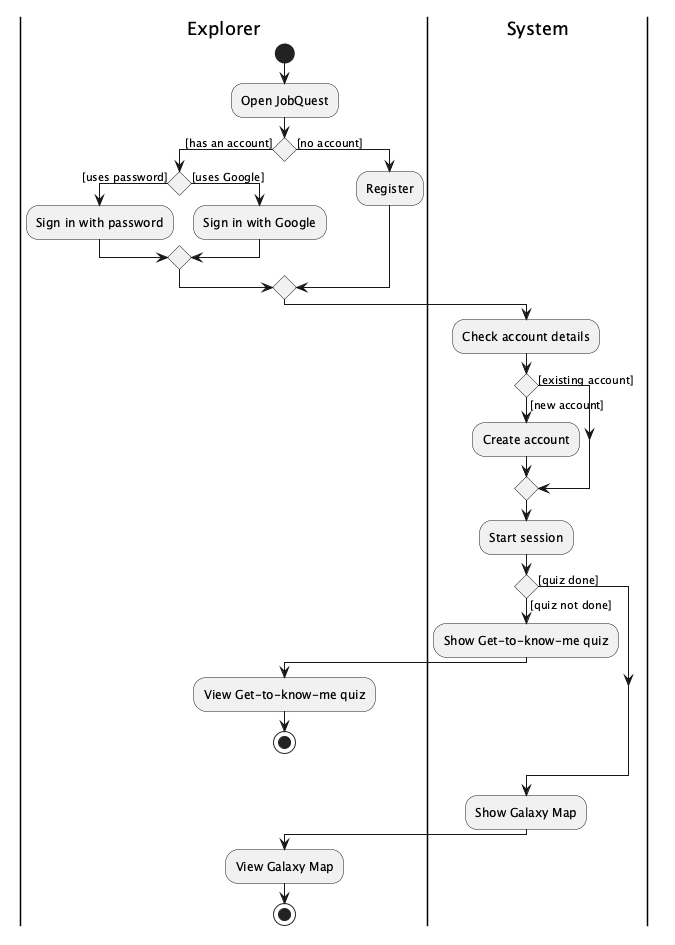
\includegraphics[width=0.59\textwidth,height=0.85\textheight,keepaspectratio]{figures/AD-01a_Explorer_AccessPlatform.png}
\caption{Explorer: access the platform (AD-01a)}
\end{figure}

\begin{figure}[H]
\centering
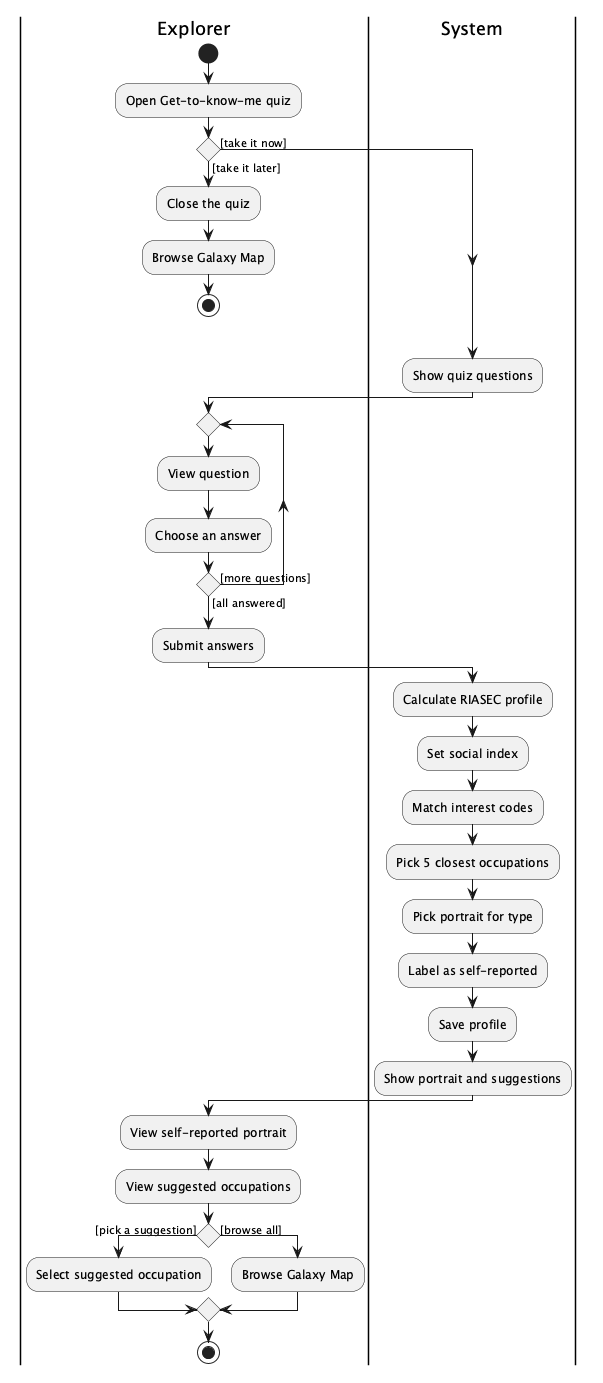
\includegraphics[width=0.53\textwidth,height=0.85\textheight,keepaspectratio]{figures/AD-01b_Explorer_GetToKnowMeQuiz.png}
\caption{Explorer: complete the Get-\allowbreak{}to-\allowbreak{}know-\allowbreak{}me quiz (AD-01b)}
\end{figure}

\begin{figure}[H]
\centering
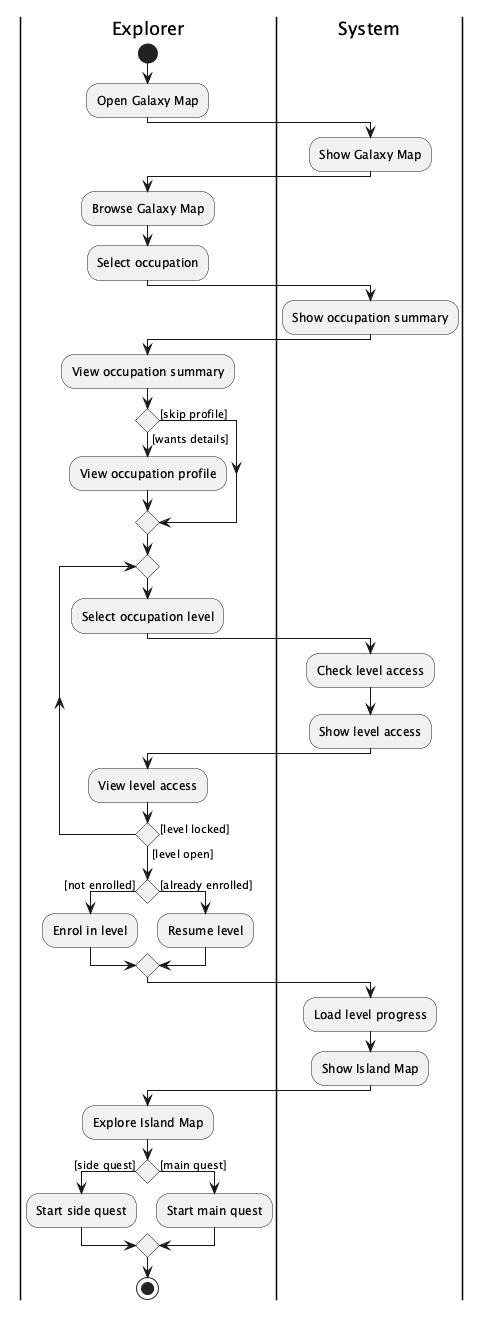
\includegraphics[width=0.43\textwidth,height=0.85\textheight,keepaspectratio]{figures/AD-01c_Explorer_ChooseLevelAndQuest.png}
\caption{Explorer: choose level and quest (AD-01c)}
\end{figure}

\begin{figure}[H]
\centering
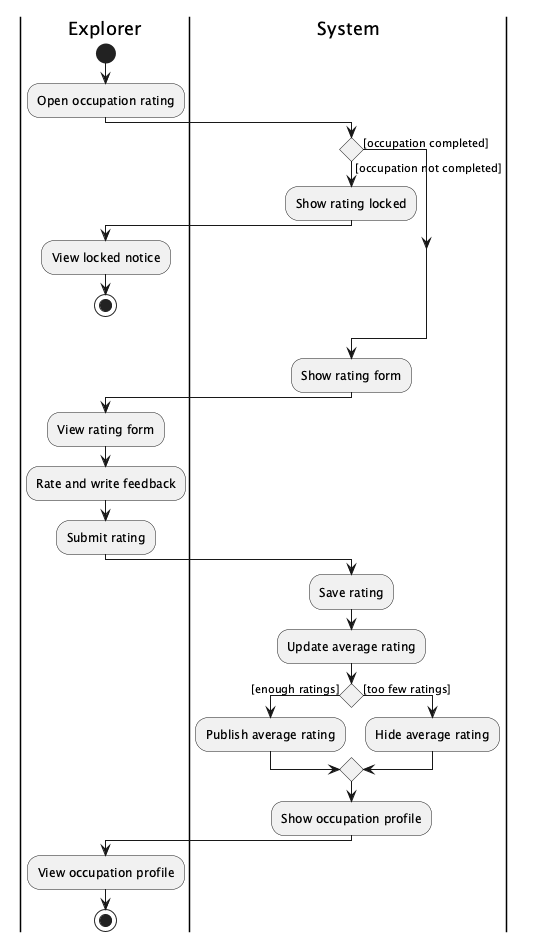
\includegraphics[width=0.47\textwidth,height=0.85\textheight,keepaspectratio]{figures/AD-01e_Explorer_RateOccupation.png}
\caption{Explorer: rate occupation (AD-01e)}
\end{figure}

\begin{figure}[H]
\centering
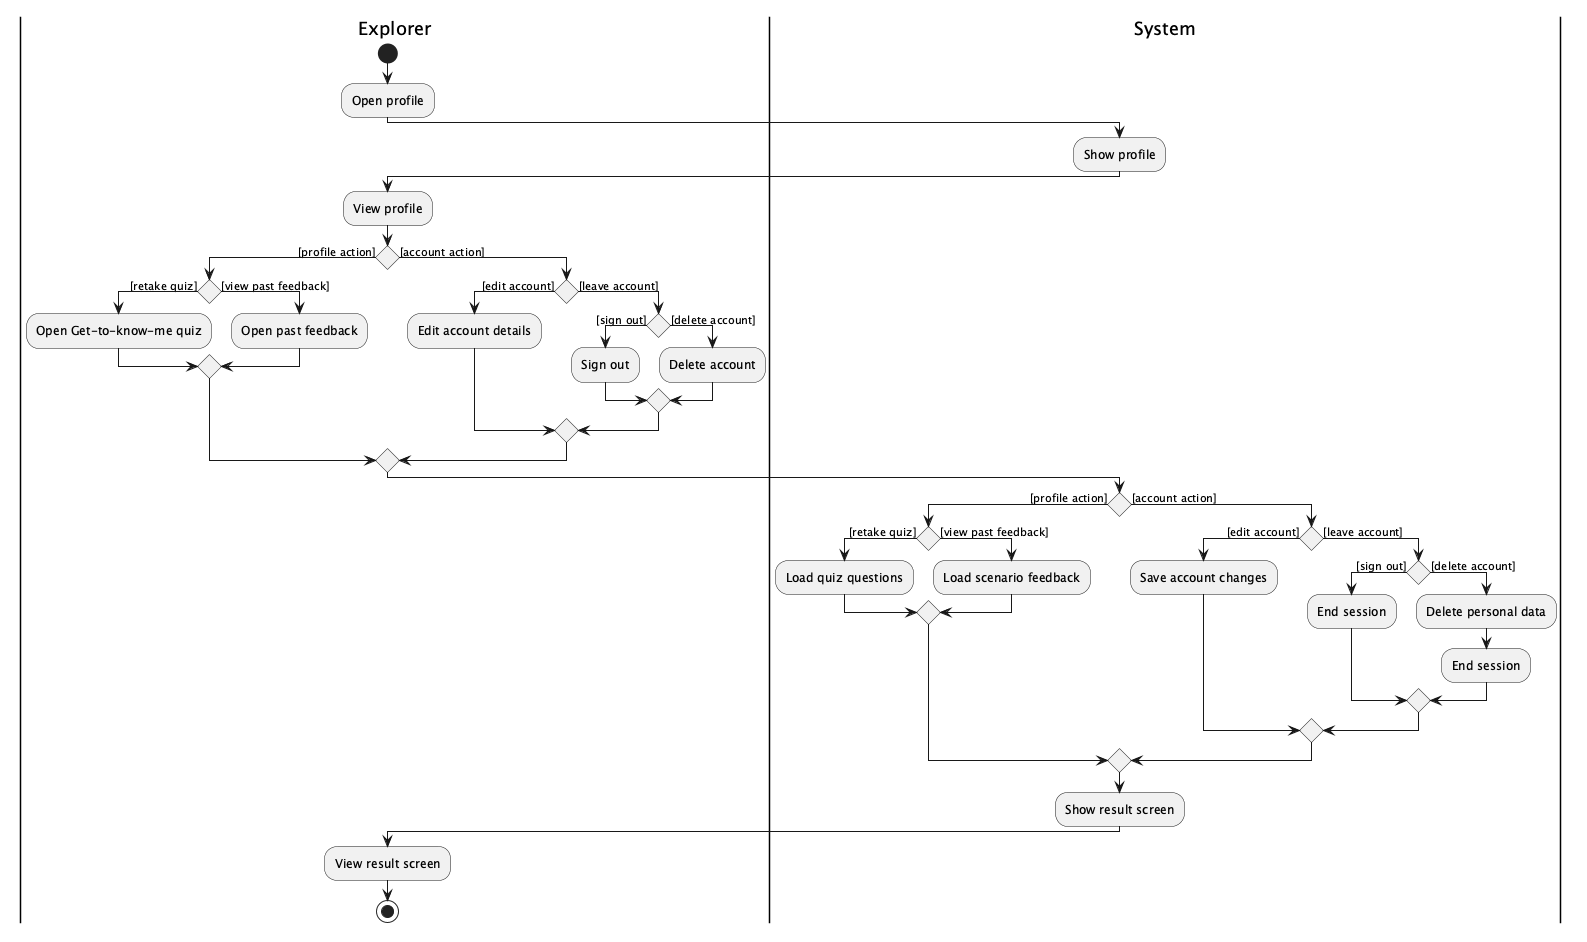
\includegraphics[width=\textwidth,height=0.85\textheight,keepaspectratio]{figures/AD-01f_Explorer_ProfileAccount.png}
\caption{Explorer: manage profile and account (AD-01f)}
\end{figure}

\begin{figure}[H]
\centering
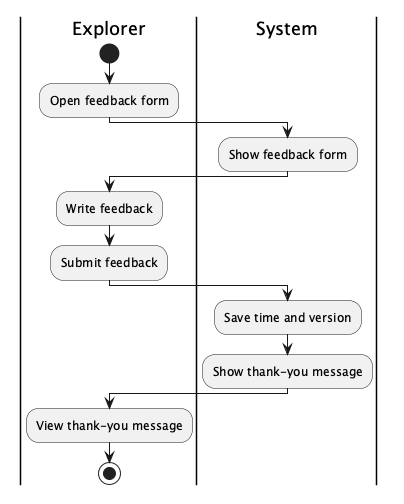
\includegraphics[width=0.35\textwidth,height=0.85\textheight,keepaspectratio]{figures/AD-01g_Explorer_SendAppFeedback.png}
\caption{Explorer: send app feedback (AD-01g)}
\end{figure}

\begin{figure}[H]
\centering
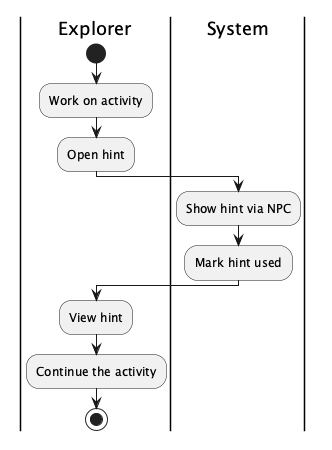
\includegraphics[width=0.35\textwidth,height=0.85\textheight,keepaspectratio]{figures/AD-01h_Explorer_ViewHint.png}
\caption{Explorer: view a hint (AD-01h)}
\end{figure}

Activity diagrams of the content administrator.

\begin{figure}[H]
\centering
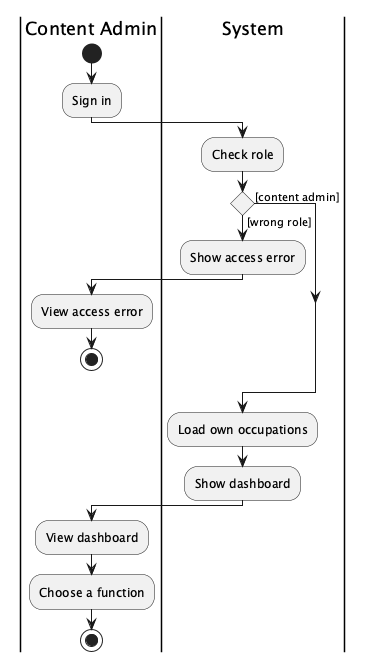
\includegraphics[width=0.36\textwidth,height=0.85\textheight,keepaspectratio]{figures/AD-02a_ContentAdmin_AccessPortal.png}
\caption{Content administrator: access the portal (AD-02a)}
\end{figure}

\begin{figure}[H]
\centering
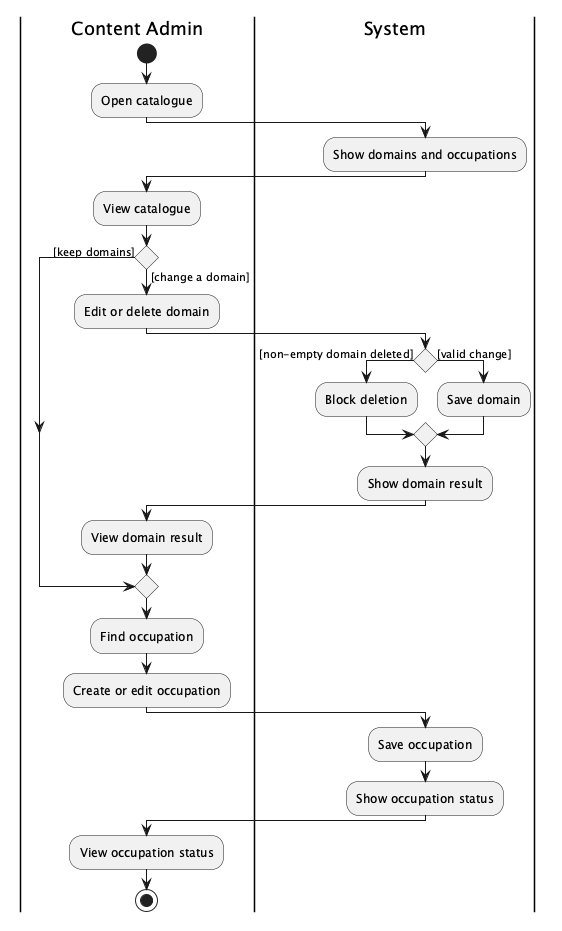
\includegraphics[width=0.49\textwidth,height=0.85\textheight,keepaspectratio]{figures/AD-02b_ContentAdmin_ManageCatalogue.png}
\caption{Content administrator: manage catalogue (AD-02b)}
\end{figure}

\begin{figure}[H]
\centering
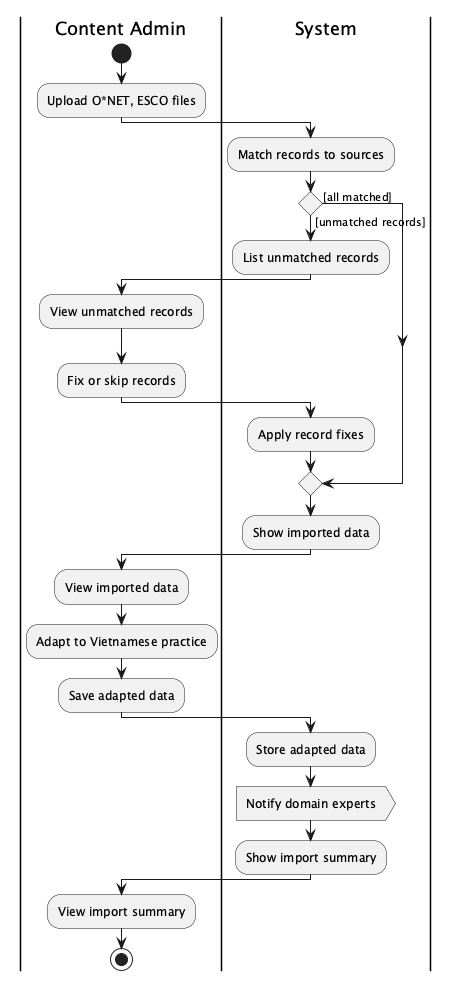
\includegraphics[width=0.4\textwidth,height=0.85\textheight,keepaspectratio]{figures/AD-02c_ContentAdmin_ImportReferenceData.png}
\caption{Content administrator: import reference data (AD-02c)}
\end{figure}

\begin{figure}[H]
\centering
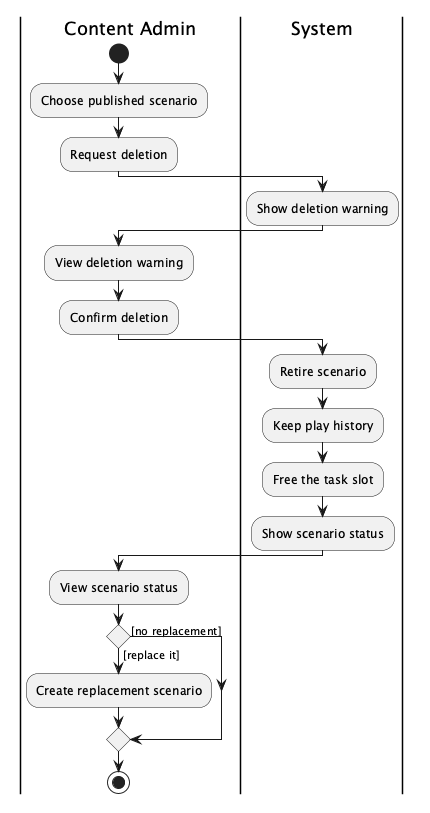
\includegraphics[width=0.38\textwidth,height=0.85\textheight,keepaspectratio]{figures/AD-02d_ContentAdmin_ReplaceOrDeleteScenario.png}
\caption{Content administrator: replace or delete scenario (AD-02d)}
\end{figure}

\begin{figure}[H]
\centering
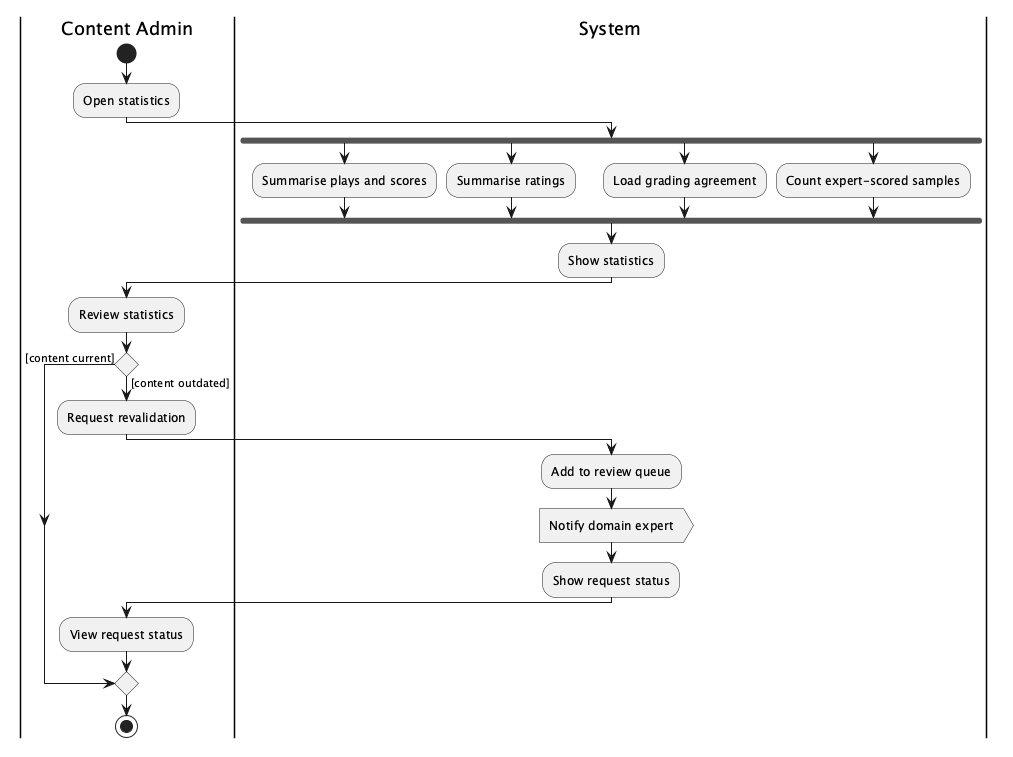
\includegraphics[width=0.89\textwidth,height=0.85\textheight,keepaspectratio]{figures/AD-02e_ContentAdmin_MonitorOccupation.png}
\caption{Content administrator: monitor occupation (AD-02e)}
\end{figure}

\begin{figure}[H]
\centering
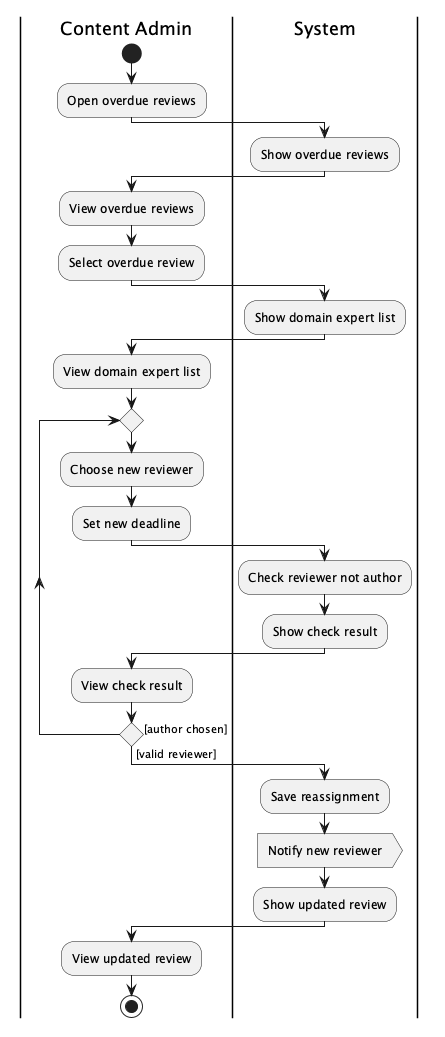
\includegraphics[width=0.39\textwidth,height=0.85\textheight,keepaspectratio]{figures/AD-02f_ContentAdmin_ReassignOverdueReview.png}
\caption{Content administrator: reassign an overdue review (AD-02f)}
\end{figure}

Activity diagrams of the domain expert.

\begin{figure}[H]
\centering
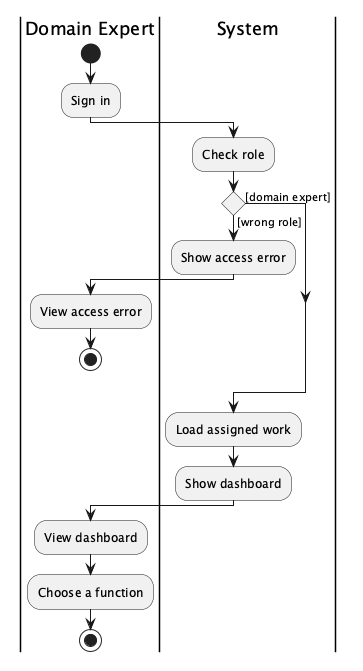
\includegraphics[width=0.35\textwidth,height=0.85\textheight,keepaspectratio]{figures/AD-03a_DomainExpert_AccessPortal.png}
\caption{Domain expert: access the portal (AD-03a)}
\end{figure}

\begin{figure}[H]
\centering
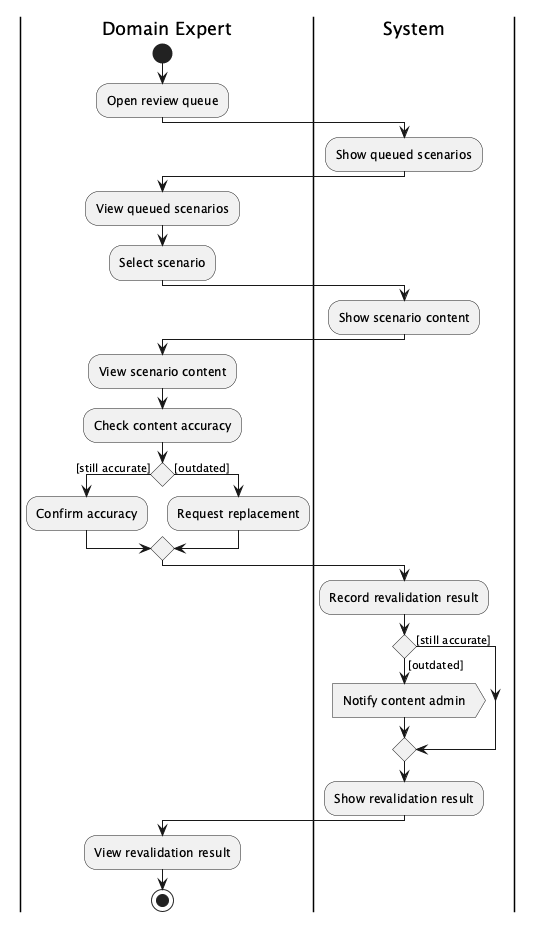
\includegraphics[width=0.47\textwidth,height=0.85\textheight,keepaspectratio]{figures/AD-03b_DomainExpert_RevalidateScenario.png}
\caption{Domain expert: revalidate scenario (AD-03b)}
\end{figure}

\begin{figure}[H]
\centering
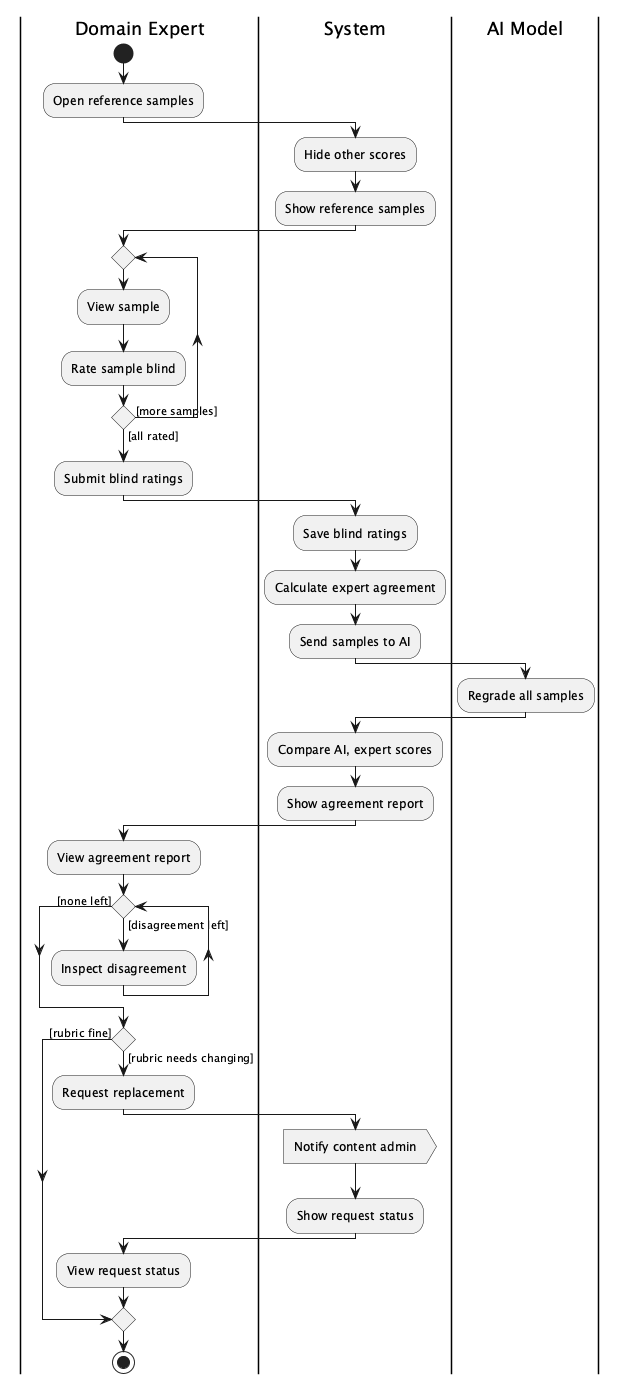
\includegraphics[width=0.55\textwidth,height=0.85\textheight,keepaspectratio]{figures/AD-03c_DomainExpert_CheckAssessorReliability.png}
\caption{Domain expert: check assessor reliability (AD-03c)}
\end{figure}

\begin{figure}[H]
\centering
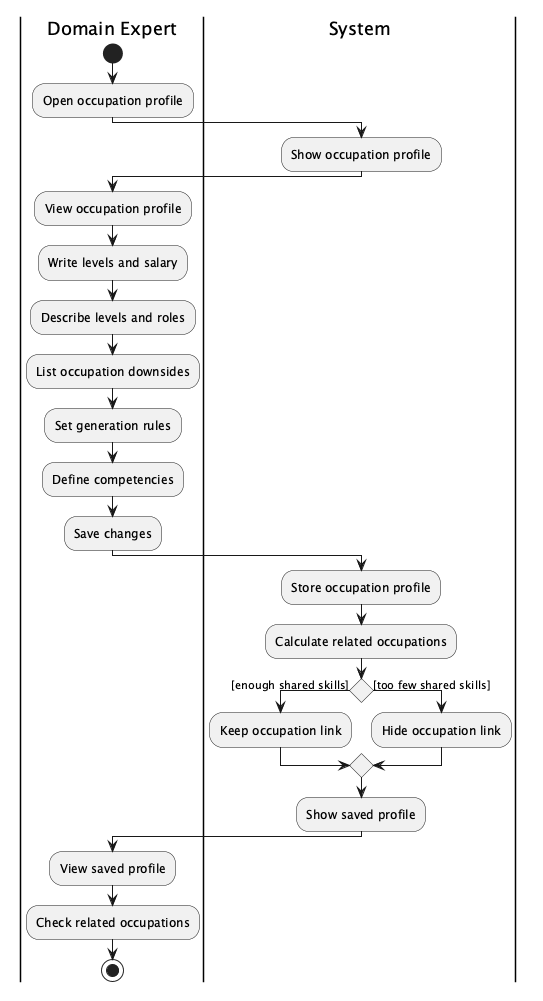
\includegraphics[width=0.47\textwidth,height=0.85\textheight,keepaspectratio]{figures/AD-03d_DomainExpert_ManageOccupationProfile.png}
\caption{Domain expert: manage occupation profile (AD-03d)}
\end{figure}

Activity diagrams of the system administrator.

\begin{figure}[H]
\centering
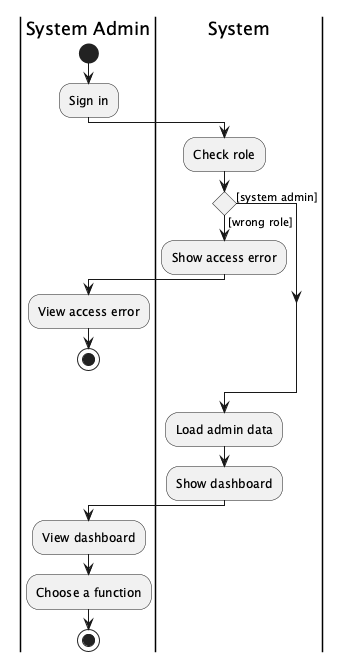
\includegraphics[width=0.35\textwidth,height=0.85\textheight,keepaspectratio]{figures/AD-05a_SystemAdmin_AccessPortal.png}
\caption{System administrator: access the portal (AD-05a)}
\end{figure}

\begin{figure}[H]
\centering
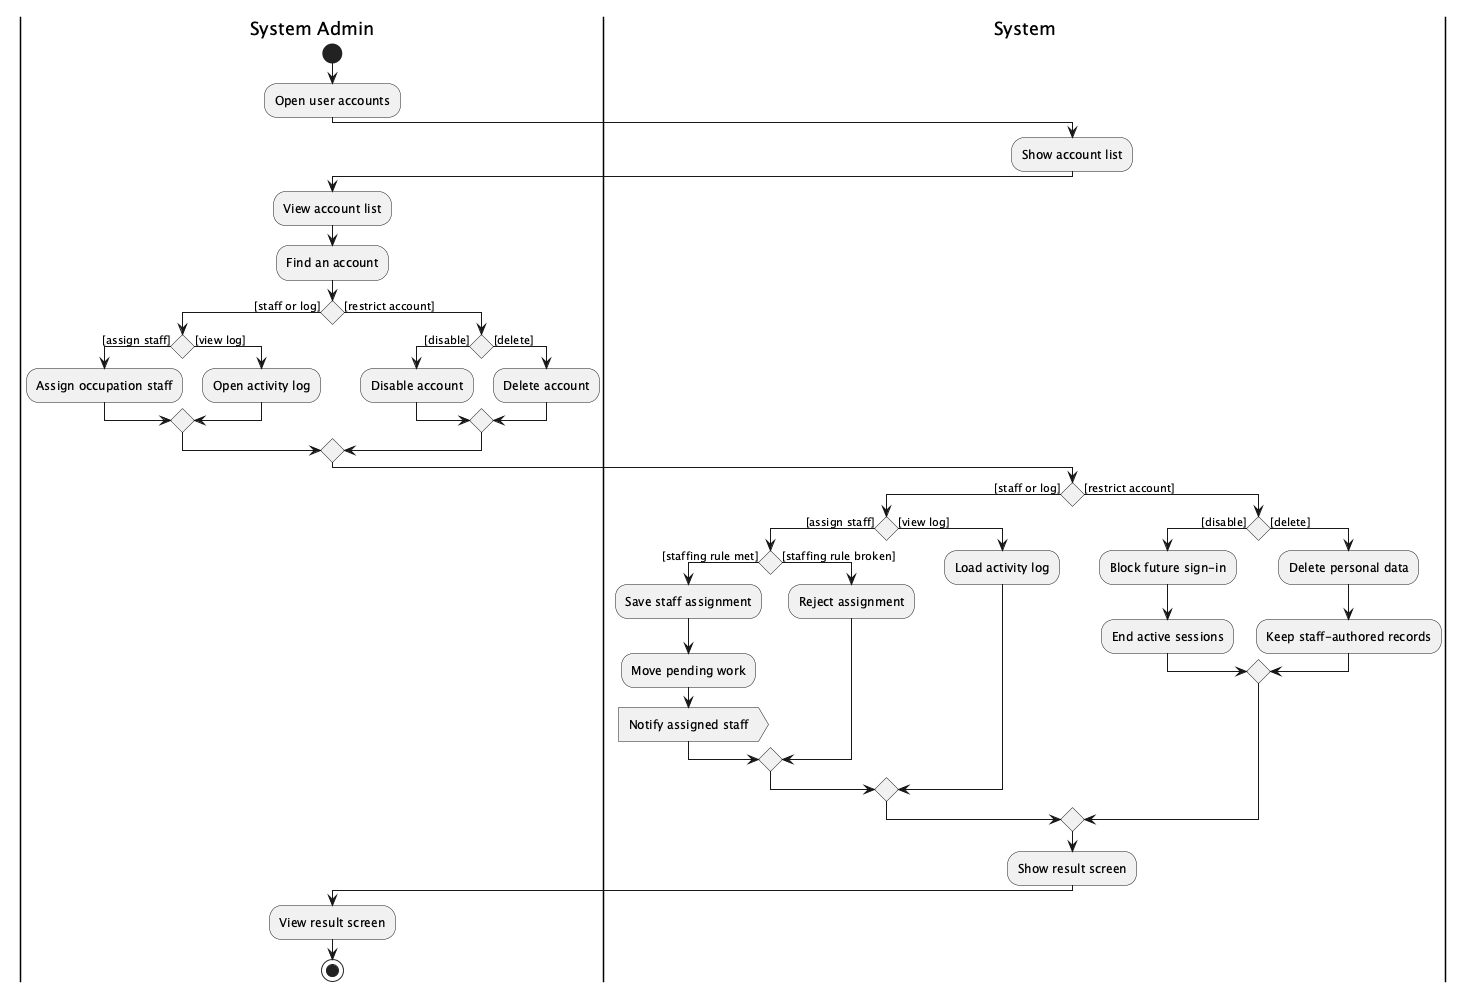
\includegraphics[width=\textwidth,height=0.85\textheight,keepaspectratio]{figures/AD-05b_SystemAdmin_ManageAccounts.png}
\caption{System administrator: manage accounts (AD-05b)}
\end{figure}

\begin{figure}[H]
\centering
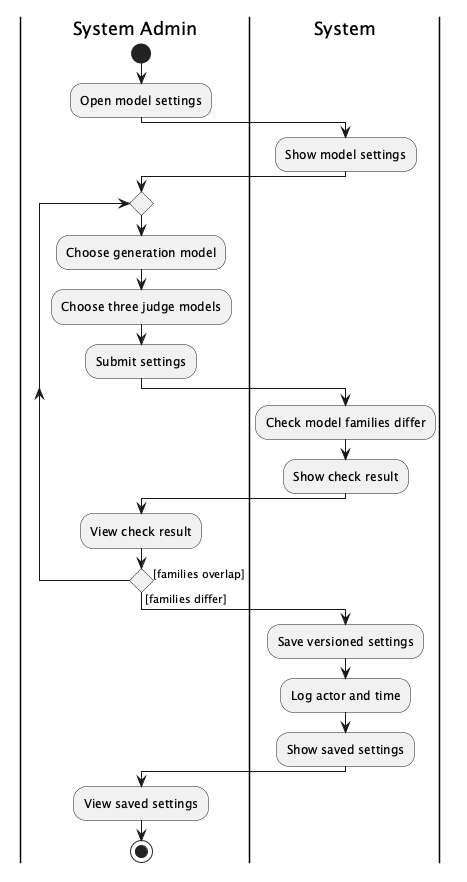
\includegraphics[width=0.4\textwidth,height=0.85\textheight,keepaspectratio]{figures/AD-05c_SystemAdmin_ConfigureModels.png}
\caption{System administrator: configure AI models (AD-05c)}
\end{figure}

\begin{figure}[H]
\centering
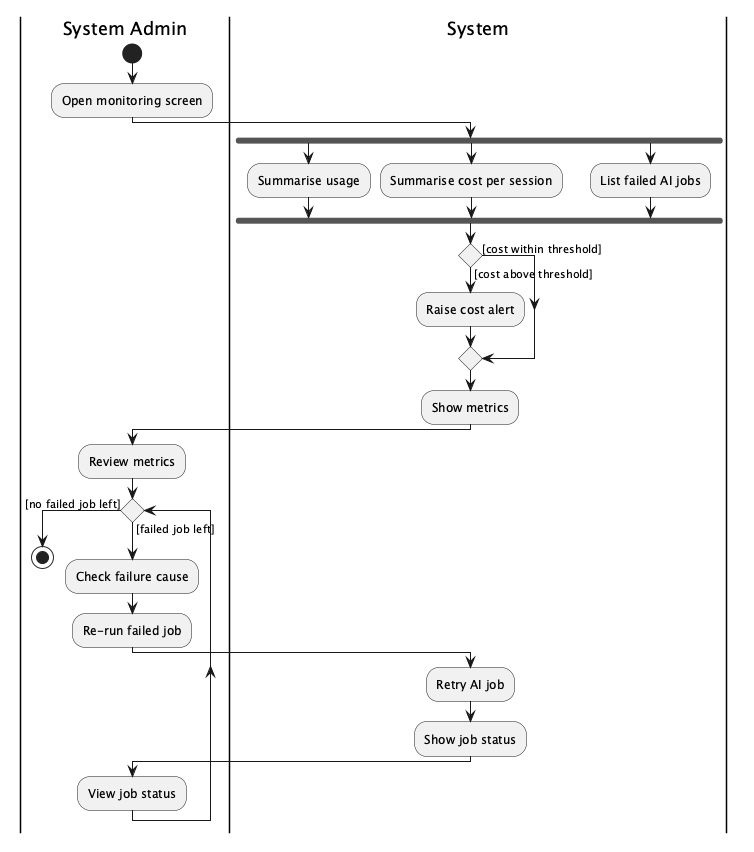
\includegraphics[width=0.66\textwidth,height=0.85\textheight,keepaspectratio]{figures/AD-05d_SystemAdmin_MonitorOperation.png}
\caption{System administrator: monitor operation (AD-05d)}
\end{figure}

\begin{figure}[H]
\centering
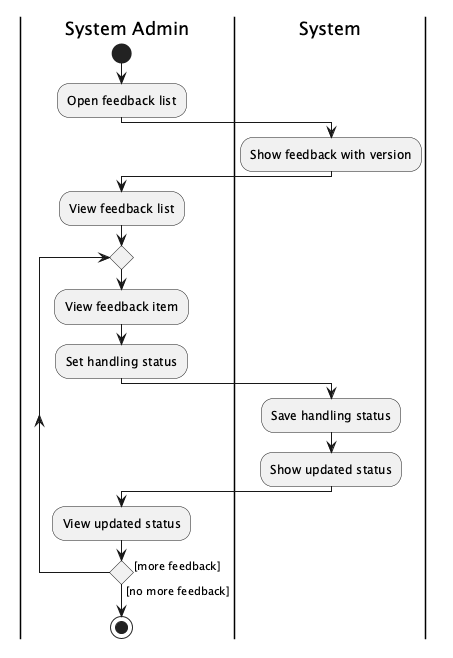
\includegraphics[width=0.4\textwidth,height=0.85\textheight,keepaspectratio]{figures/AD-05e_SystemAdmin_ReviewFeedback.png}
\caption{System administrator: review app feedback (AD-05e)}
\end{figure}

Sitemap of the staff application.

\begin{landscape}
\begin{figure}[H]
\centering
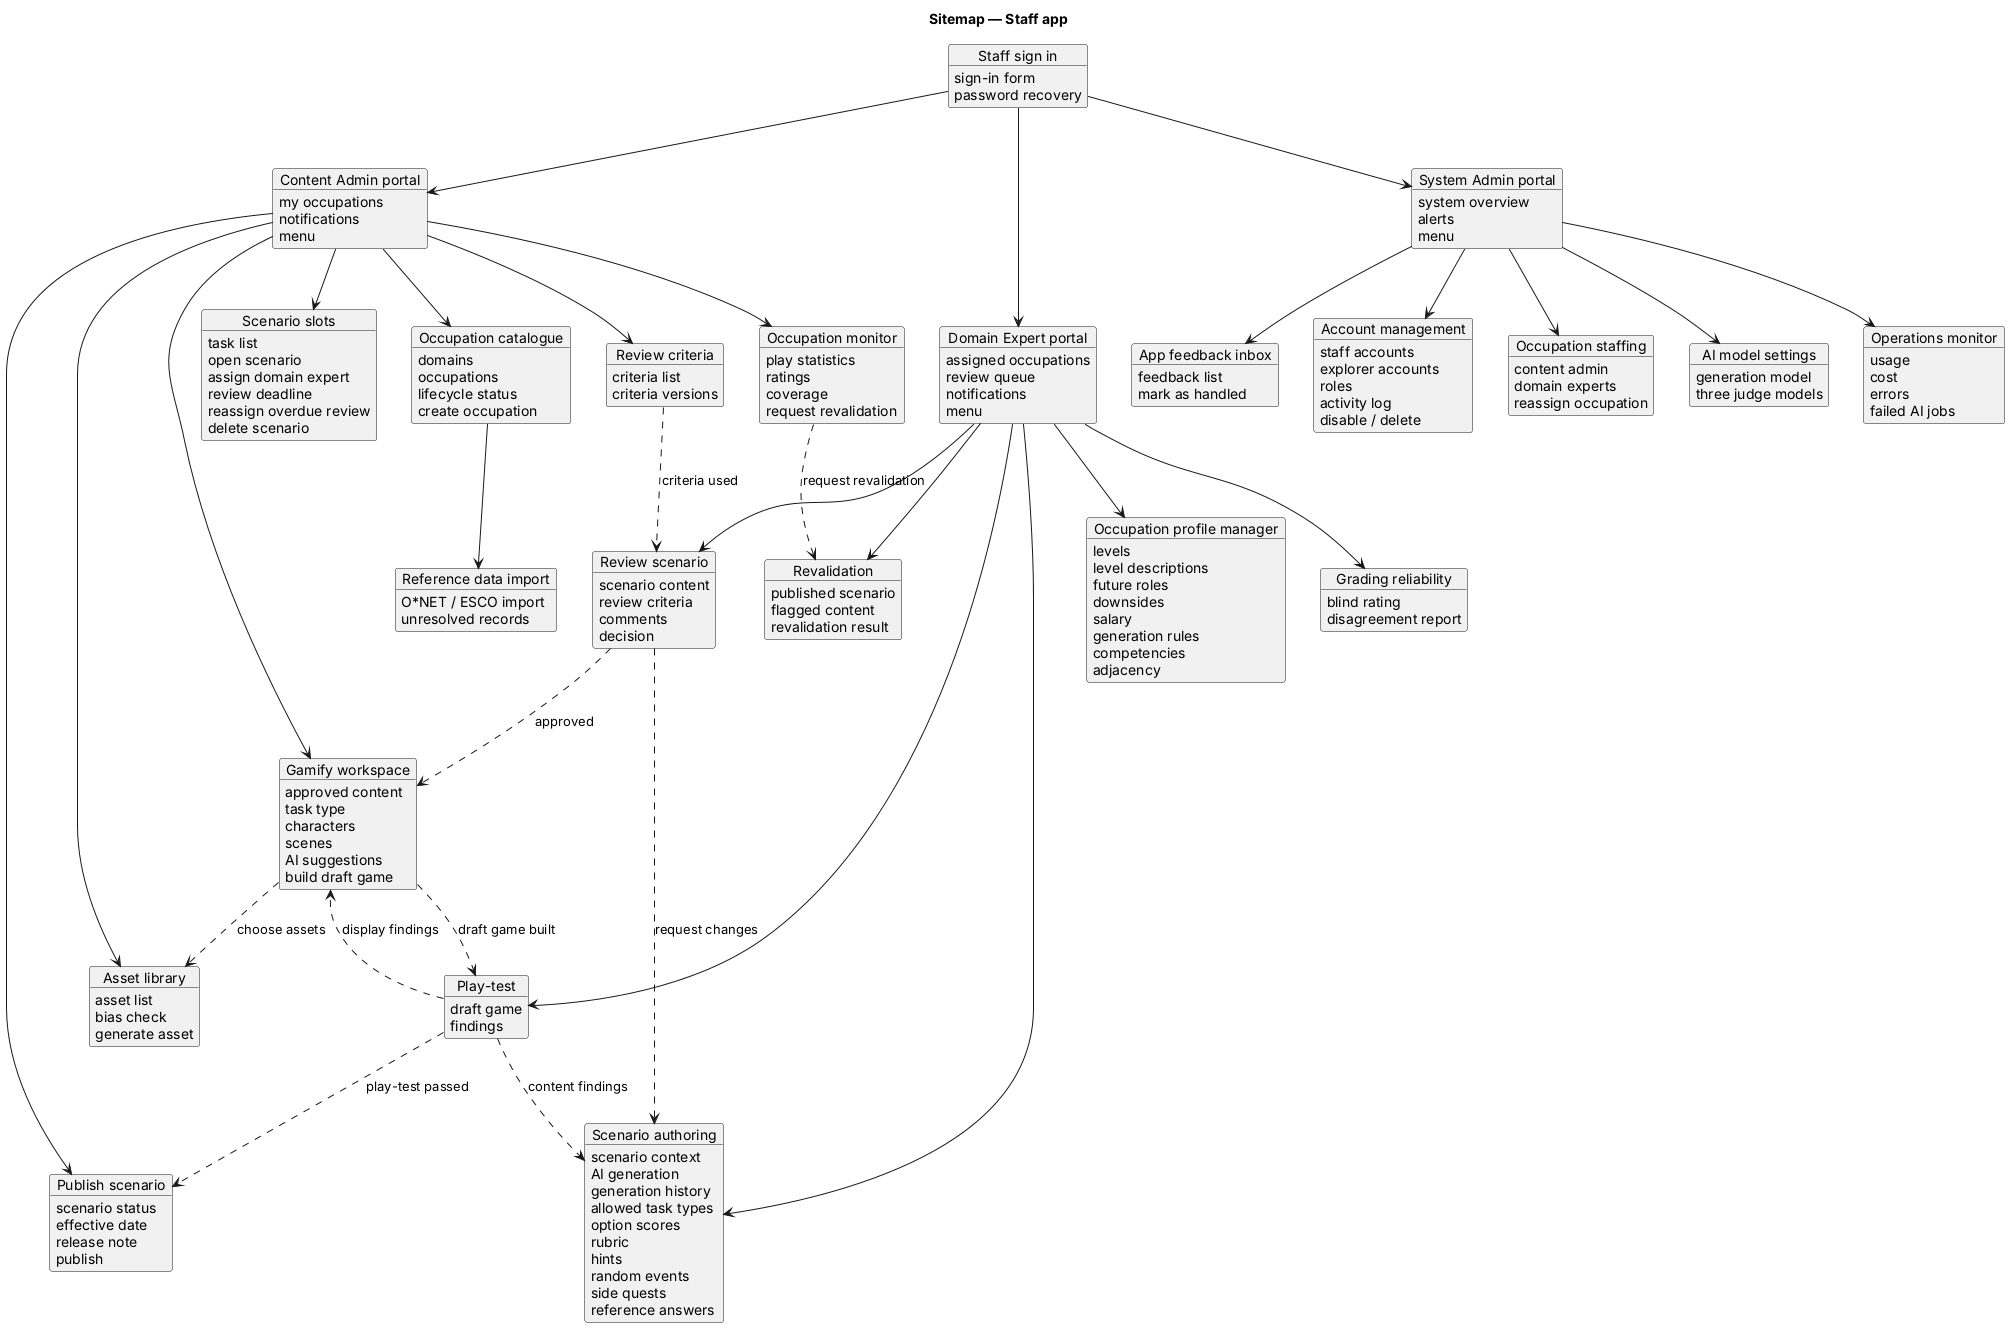
\includegraphics[width=\linewidth,height=0.86\textwidth,keepaspectratio,keepaspectratio]{figures/SITE-02_StaffApp.png}
\caption{Sitemap of the staff application (SITE-02): three portals behind one sign-in, with dashed arrows for the path a scenario takes between them}
\end{figure}
\end{landscape}

\begin{figure}[H]
\centering
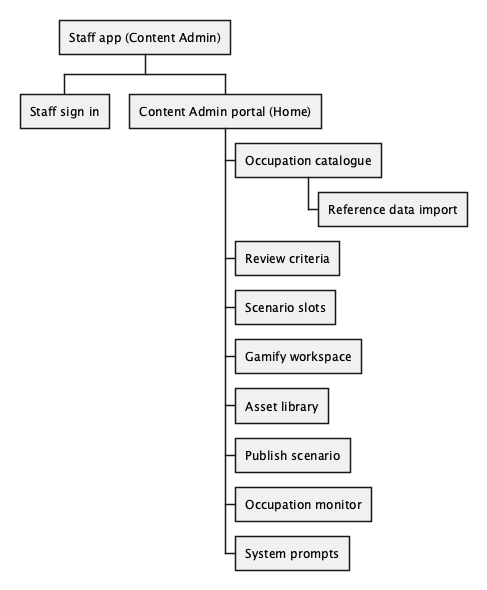
\includegraphics[width=0.8\textwidth,height=0.85\textheight,keepaspectratio]{figures/SITE-02_StaffApp_ContentAdmin.png}
\caption{Sitemap of the content administrator portal (SITE-02, content administrator)}
\end{figure}

\begin{figure}[H]
\centering
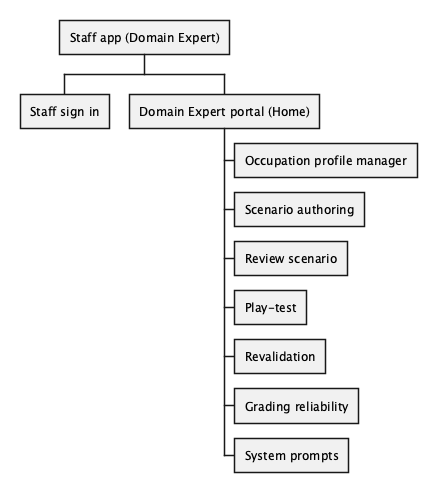
\includegraphics[width=0.8\textwidth,height=0.85\textheight,keepaspectratio]{figures/SITE-03_StaffApp_DomainExpert.png}
\caption{Sitemap of the domain expert portal (SITE-03)}
\end{figure}

\begin{figure}[H]
\centering
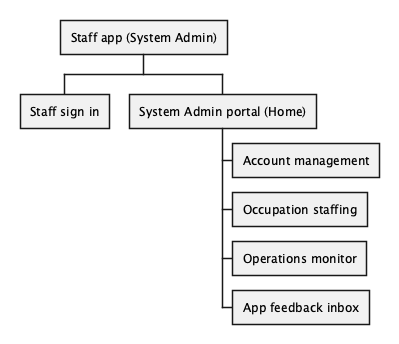
\includegraphics[width=0.8\textwidth,height=0.85\textheight,keepaspectratio]{figures/SITE-04_StaffApp_SystemAdmin.png}
\caption{Sitemap of the system administrator portal (SITE-04)}
\end{figure}

Sequence diagrams.

\begin{figure}[H]
\centering
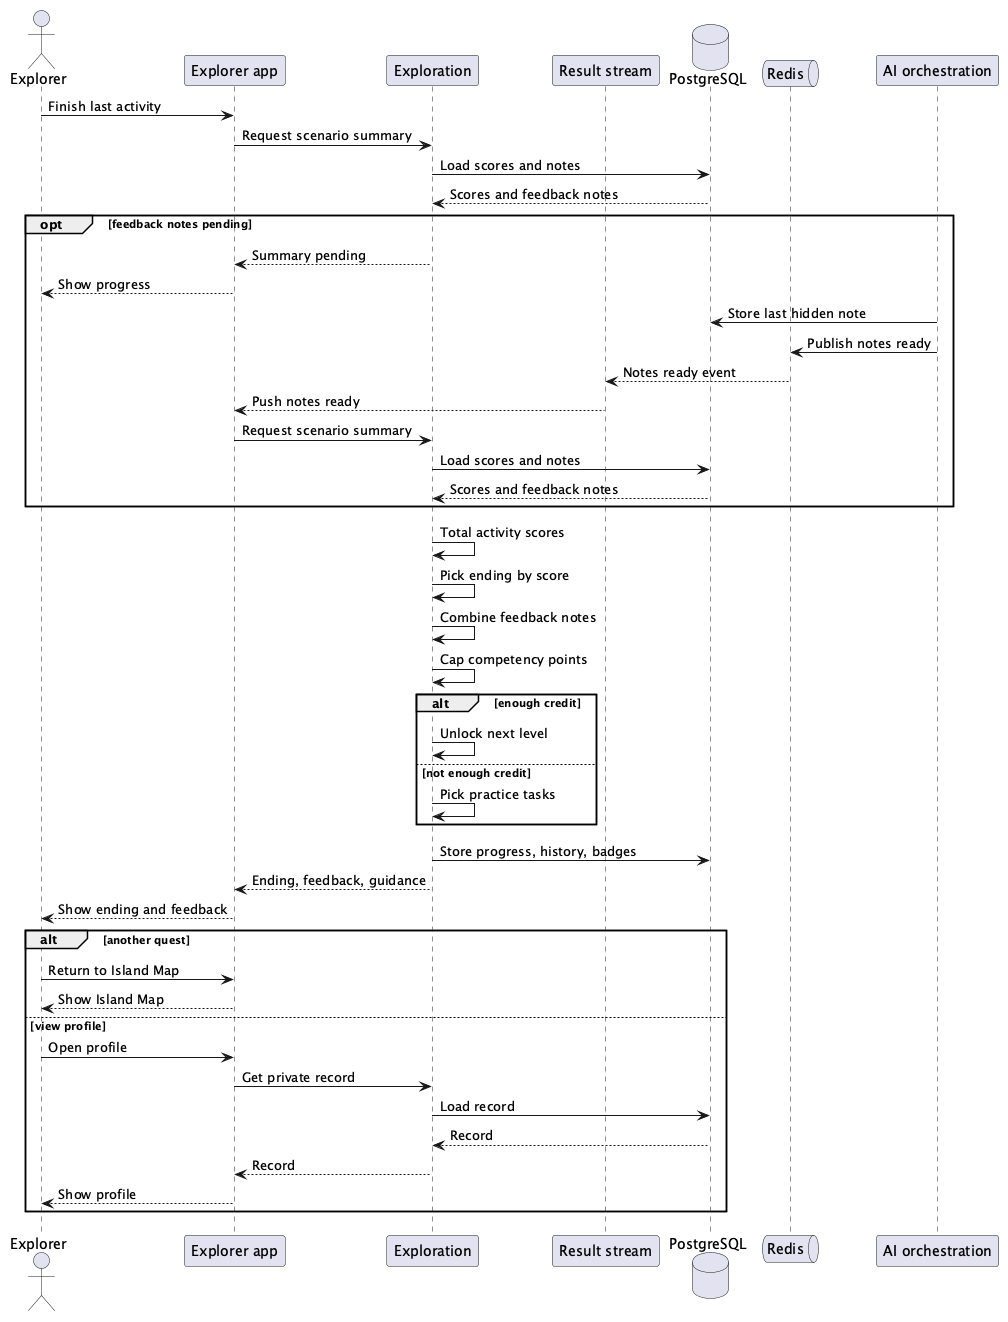
\includegraphics[width=0.92\textwidth,height=0.85\textheight,keepaspectratio]{figures/SD-02_Explorer_FinishScenario.png}
\caption{Sequence of finishing a scenario (SD-02): waiting for pending feedback notes, scoring, credit and unlocking, and the summary}
\end{figure}

\begin{figure}[H]
\centering
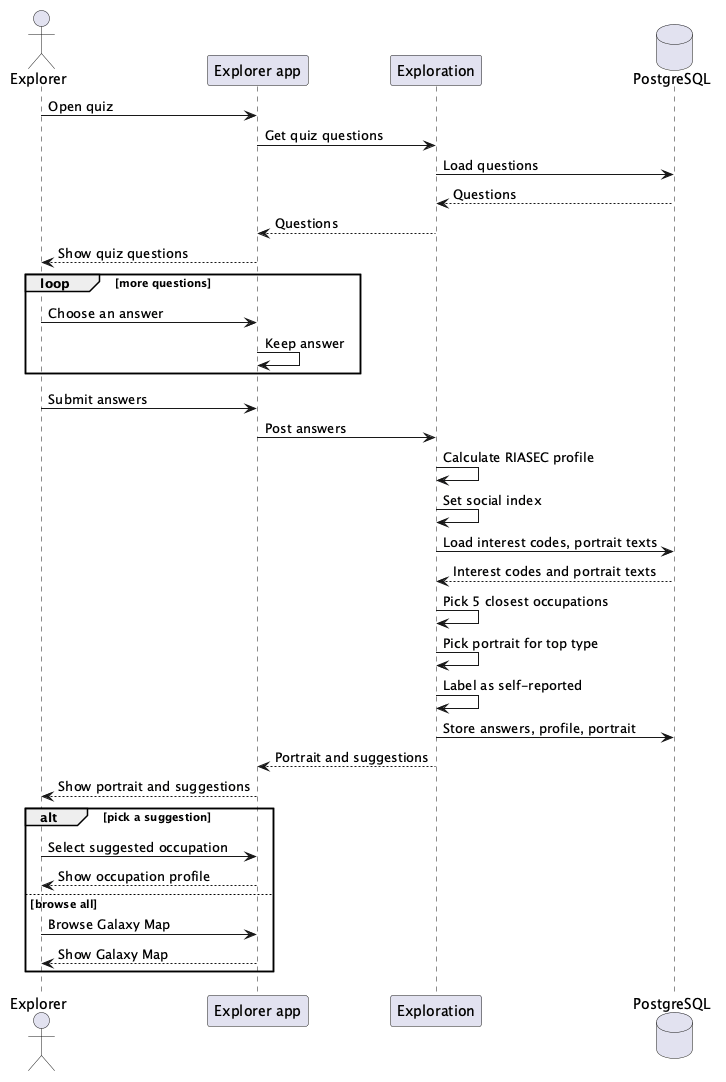
\includegraphics[width=0.64\textwidth,height=0.85\textheight,keepaspectratio]{figures/SD-03_Explorer_GetToKnowMeQuiz.png}
\caption{Sequence of the Get-\allowbreak{}to-\allowbreak{}know-\allowbreak{}me quiz (SD-03): profile, suggestions, and portrait computed without AI}
\end{figure}

\begin{figure}[H]
\centering
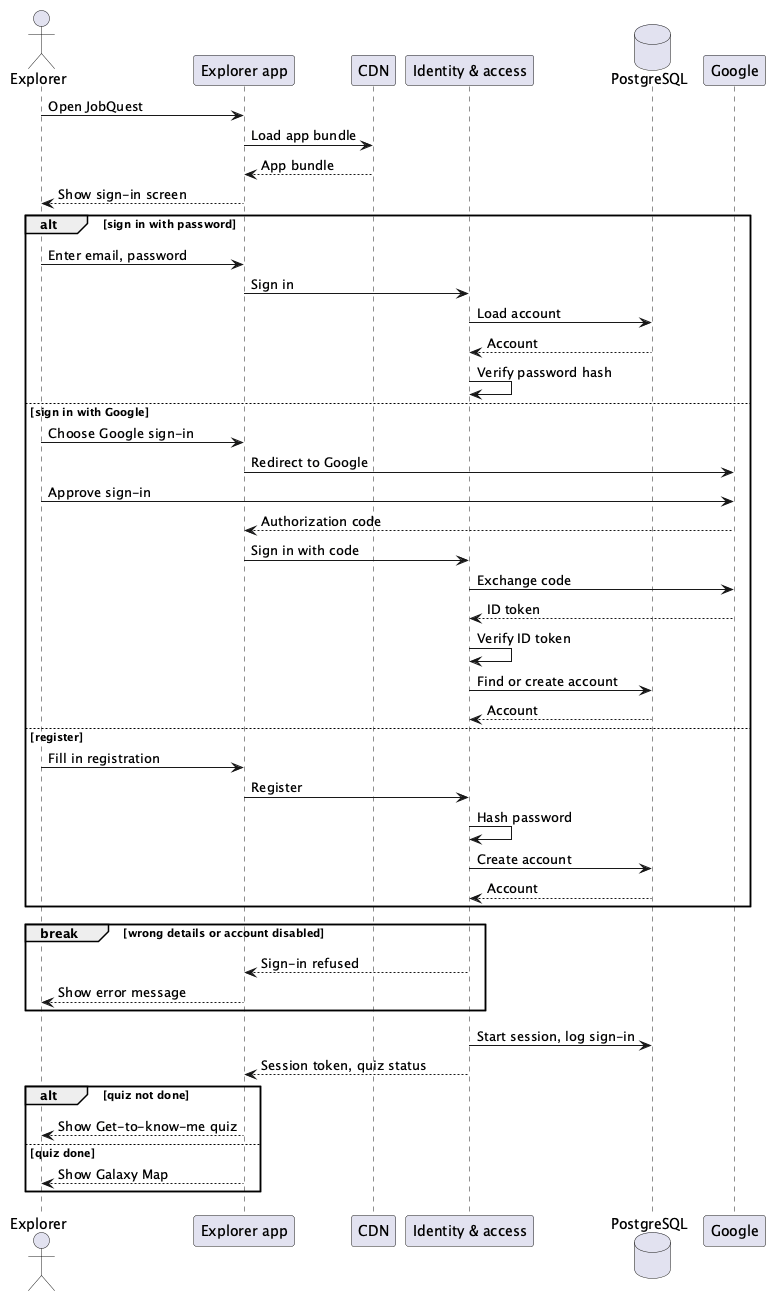
\includegraphics[width=0.7\textwidth,height=0.85\textheight,keepaspectratio]{figures/SD-04_Explorer_AccessPlatform.png}
\caption{Sequence of access to the platform (SD-04): sign-in with a password or Google, or registration, then the quiz or the Galaxy Map}
\end{figure}

\begin{figure}[H]
\centering
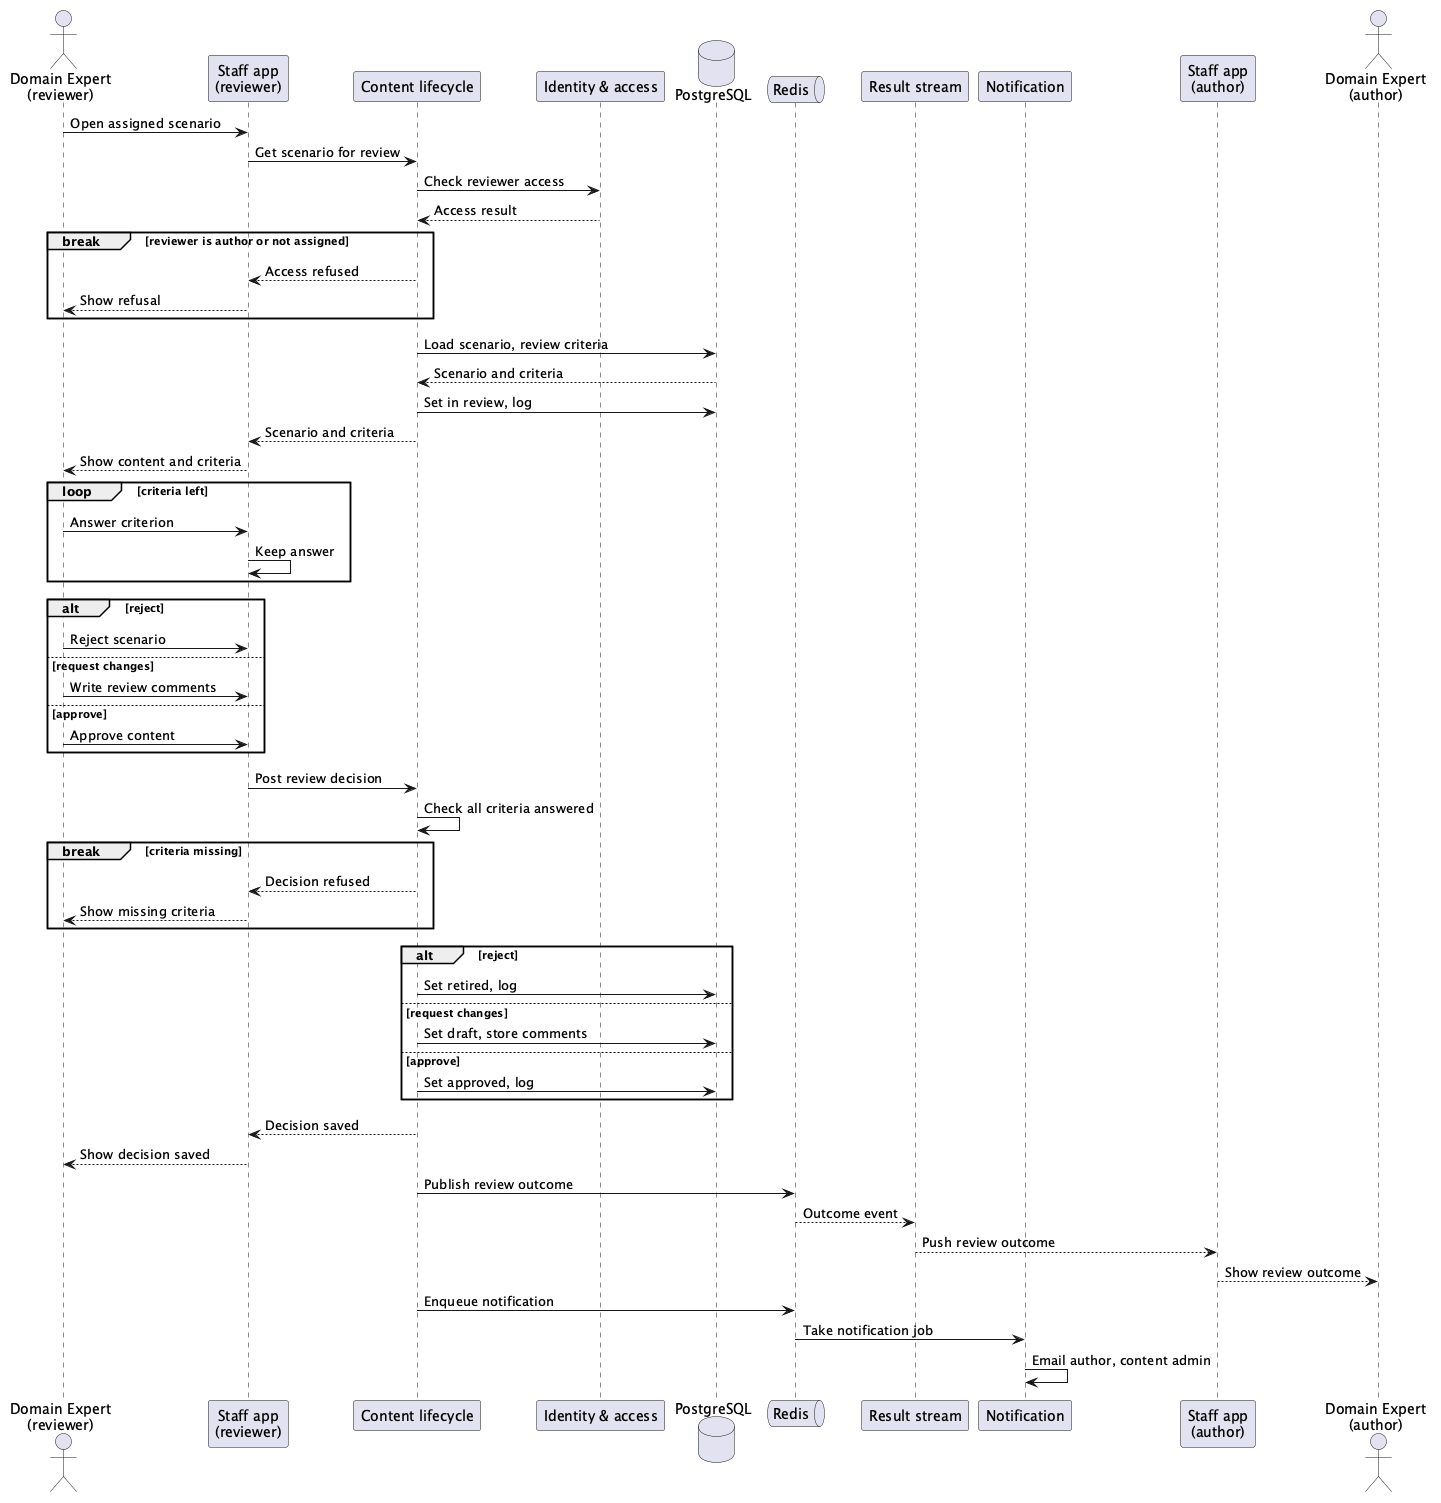
\includegraphics[width=\textwidth,height=0.9\textheight,keepaspectratio]{figures/SD-06_DomainExpert_ReviewScenario.png}
\caption{Sequence of reviewing a scenario (SD-06): access check, answers to the review criteria, and the decision with its state change}
\end{figure}

\begin{figure}[H]
\centering
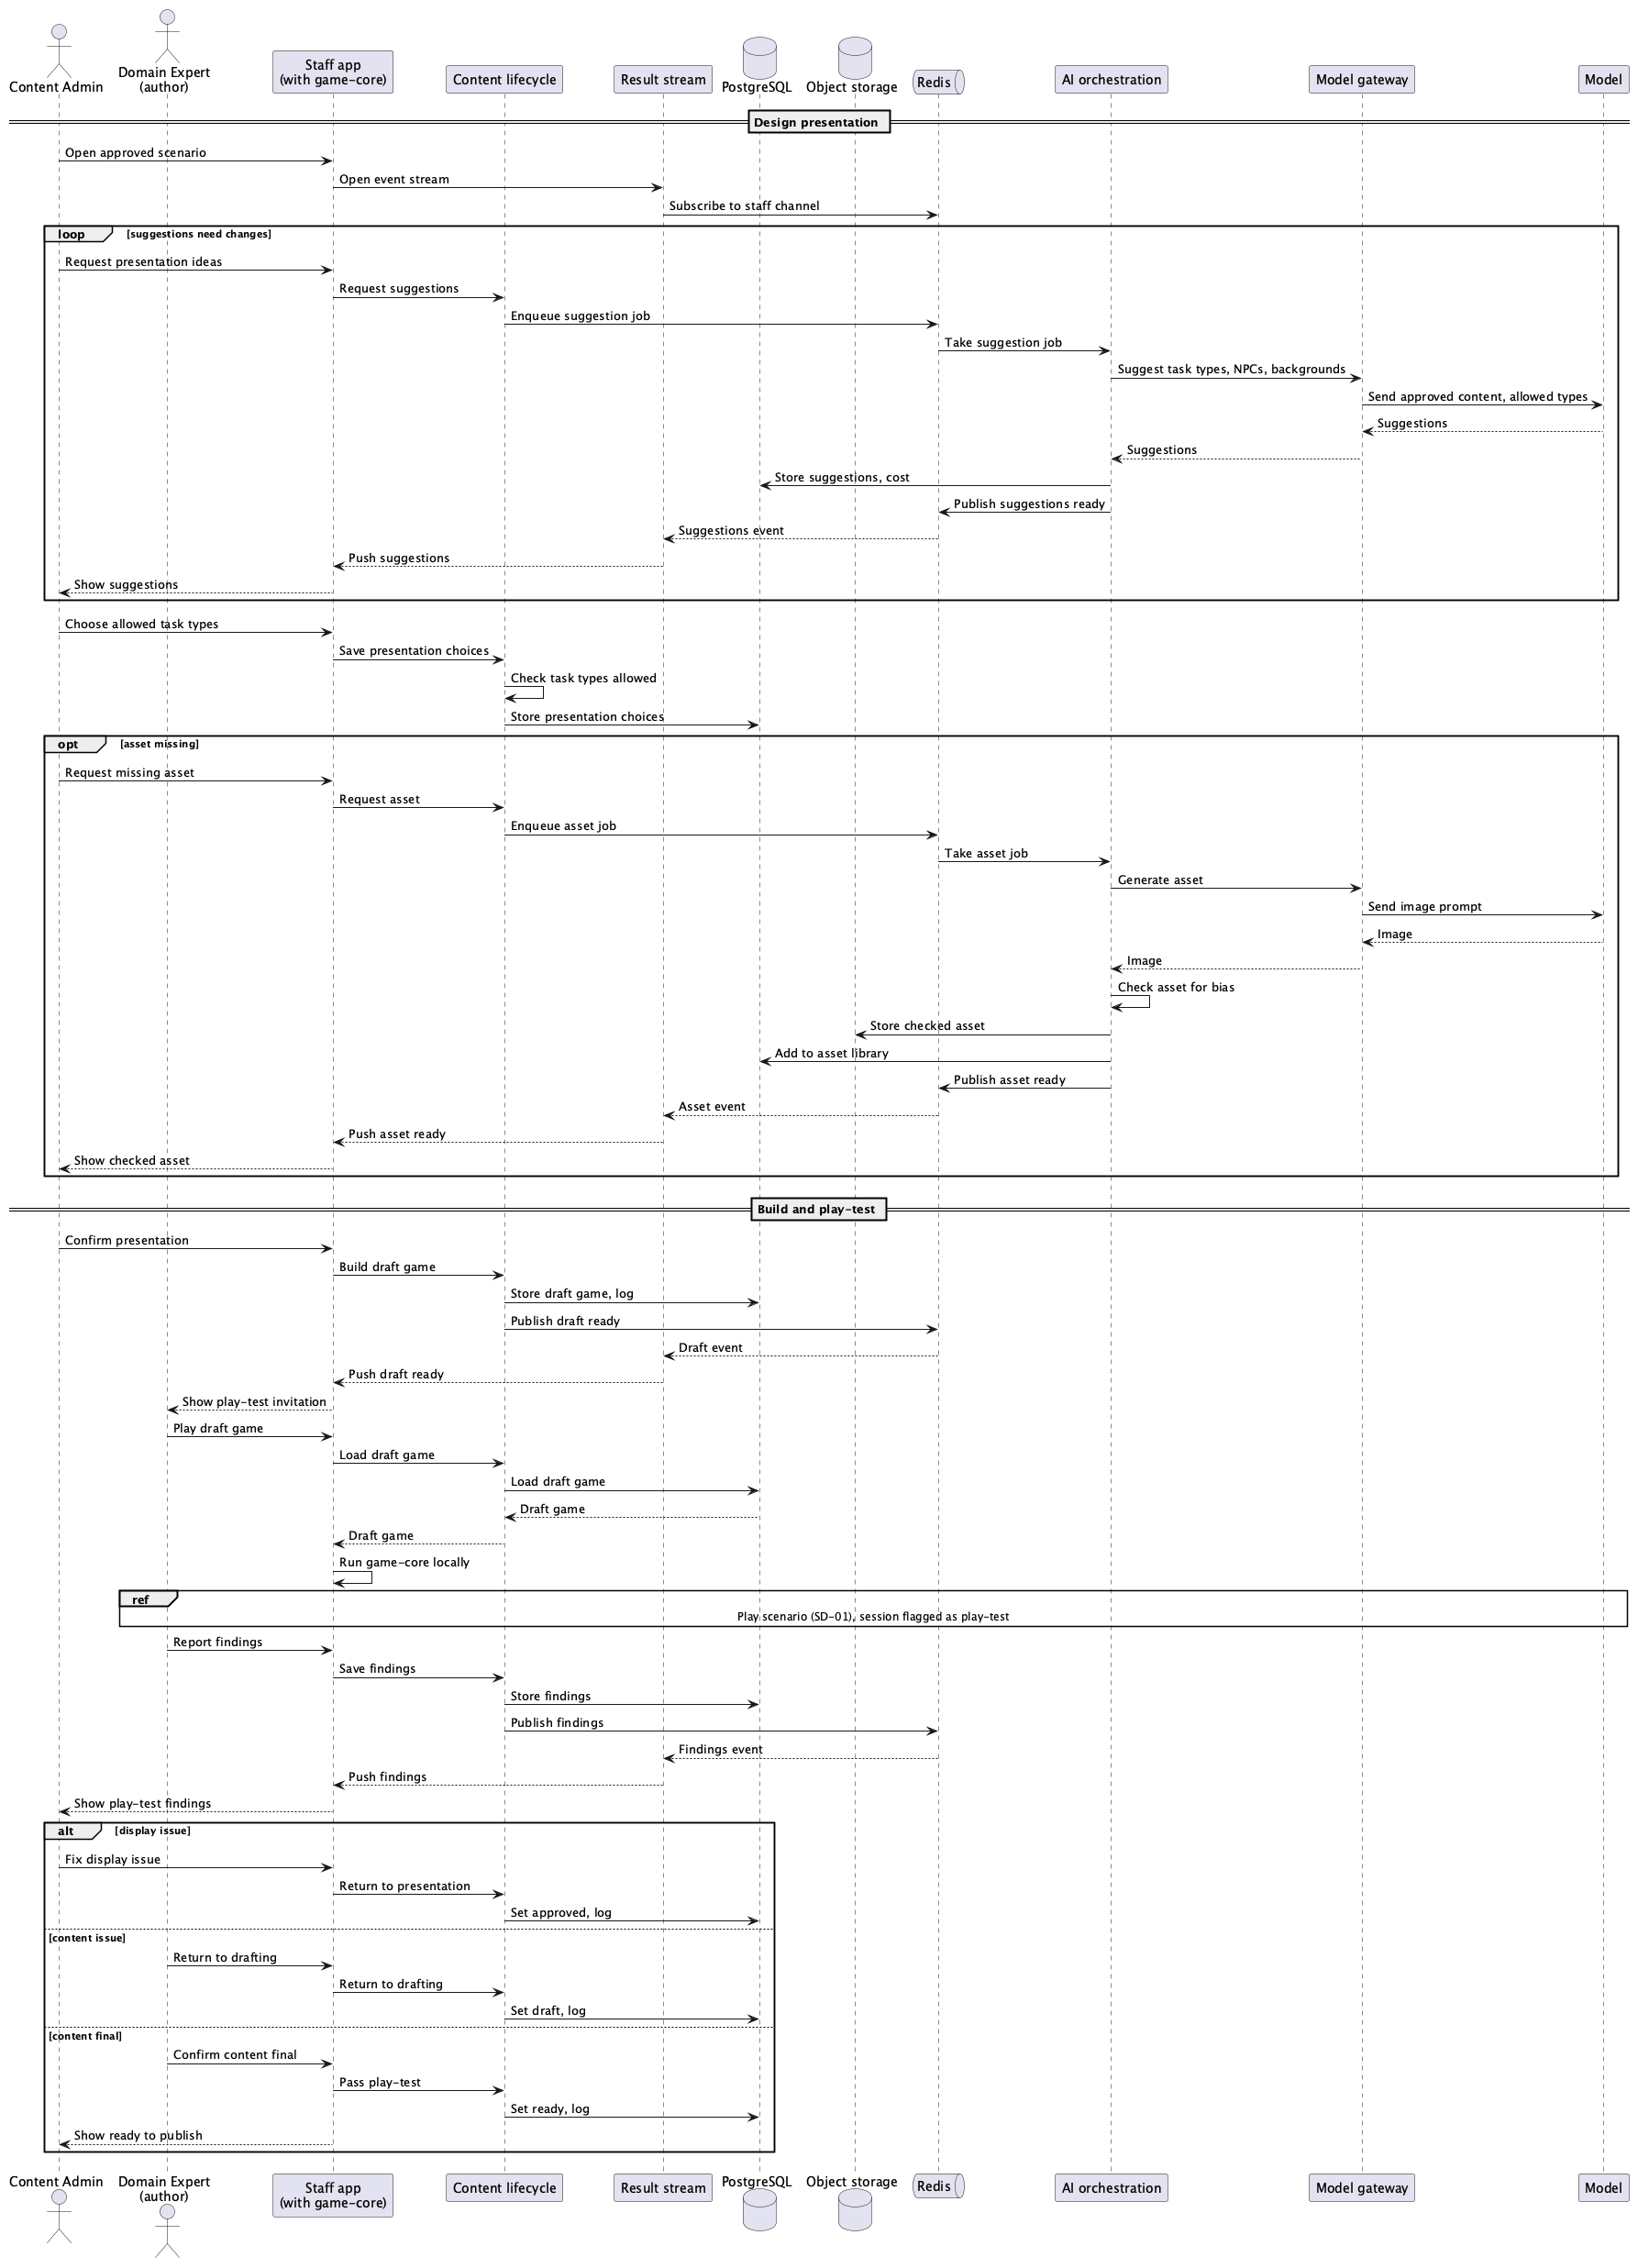
\includegraphics[width=\textwidth,height=0.9\textheight,keepaspectratio]{figures/SD-07_ContentAdmin_GamifyAndPlaytest.png}
\caption{Sequence of gamifying and play-\allowbreak{}testing a scenario (SD-07): presentation suggested with AI, missing assets generated and checked, and the draft game play-tested by its author}
\end{figure}

\begin{figure}[H]
\centering
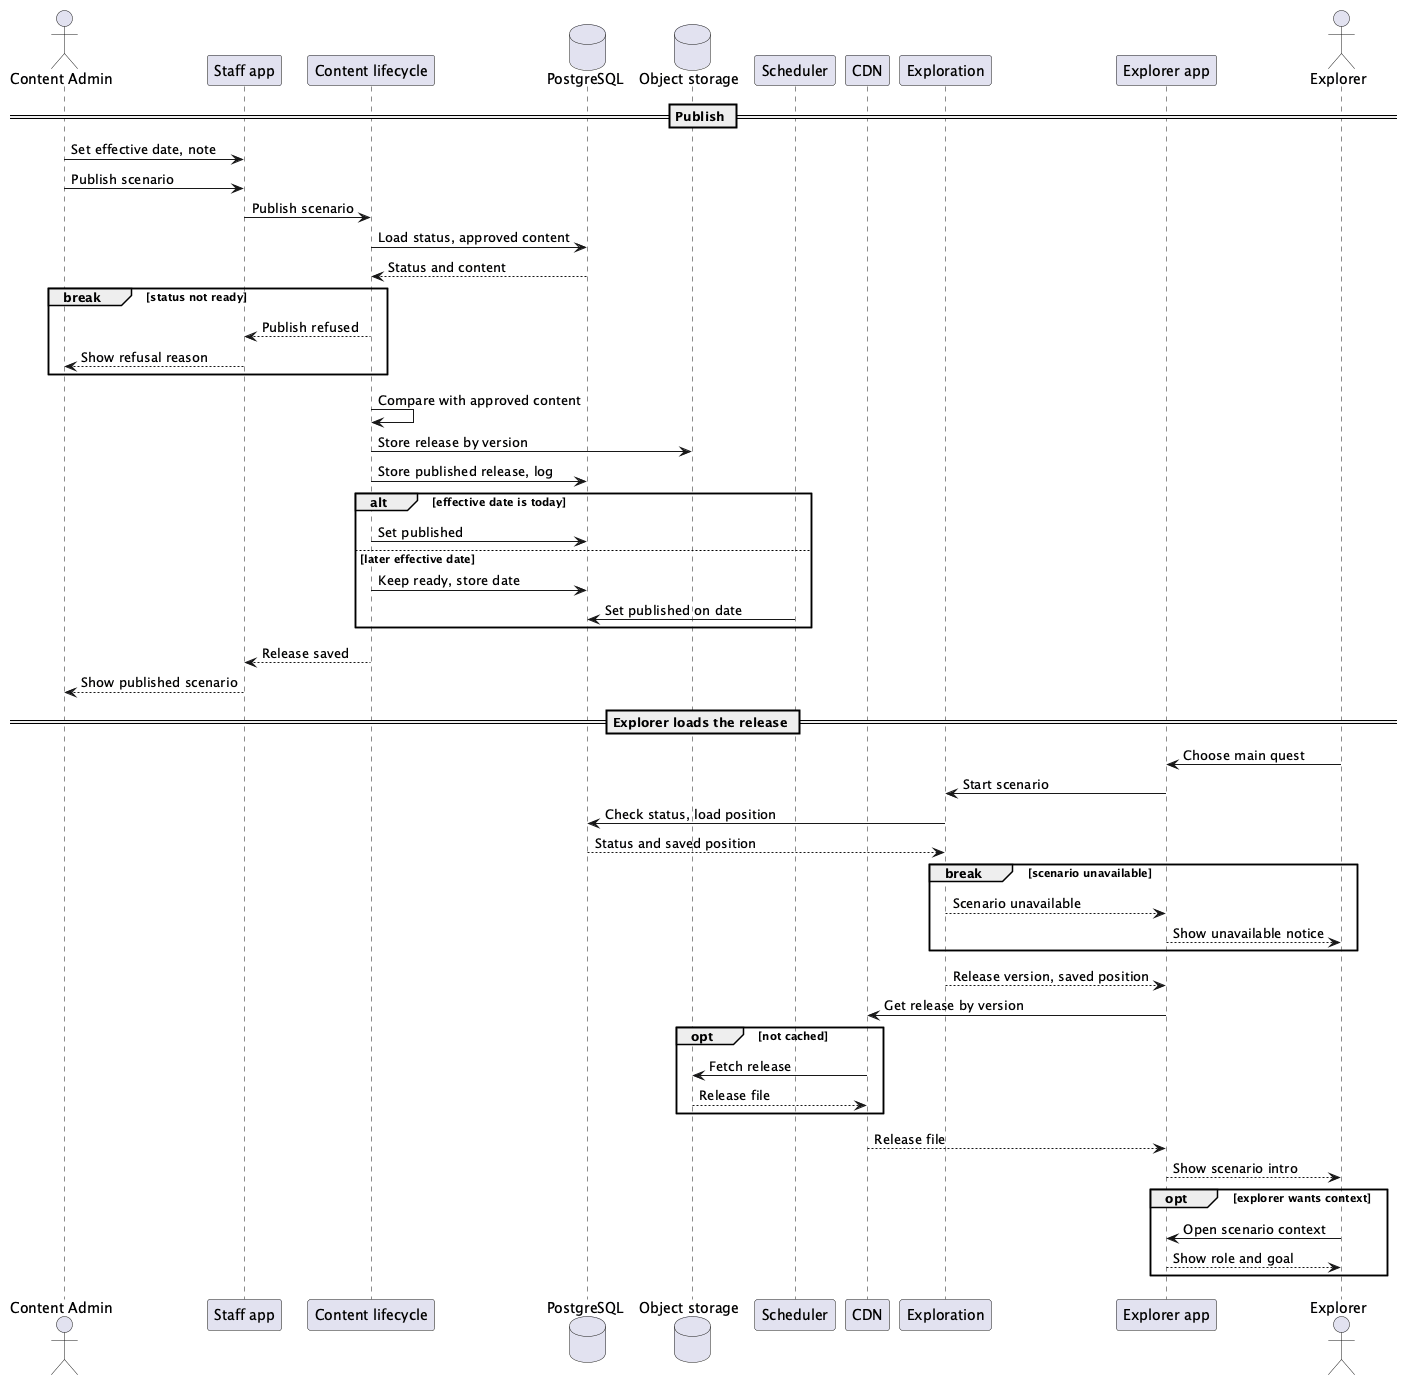
\includegraphics[width=\textwidth,height=0.9\textheight,keepaspectratio]{figures/SD-08_ContentAdmin_PublishScenario.png}
\caption{Sequence of publishing a scenario (SD-08): checks and the immutable release, publication on the effective date, and the explorer loading the release through the content delivery network}
\end{figure}

\begin{figure}[H]
\centering
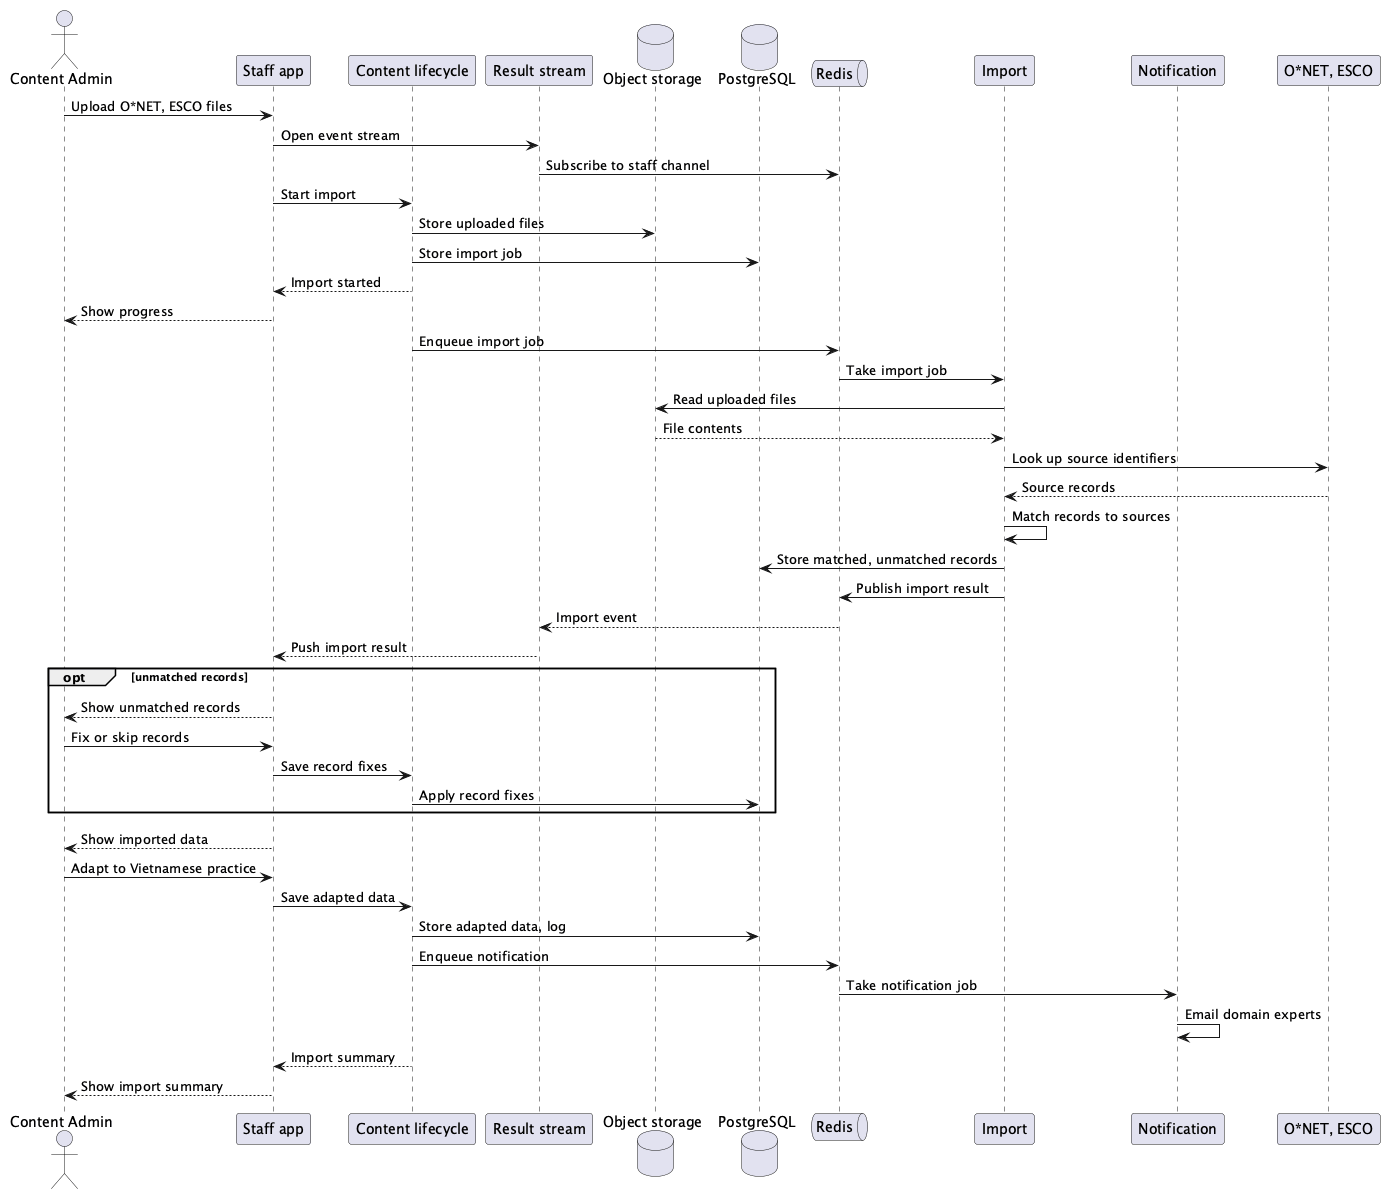
\includegraphics[width=\textwidth,height=0.9\textheight,keepaspectratio]{figures/SD-09_ContentAdmin_ImportReferenceData.png}
\caption{Sequence of importing reference data (SD-09): upload, matching against O*NET and ESCO, resolution of unmatched records, and adaptation}
\end{figure}

\begin{figure}[H]
\centering
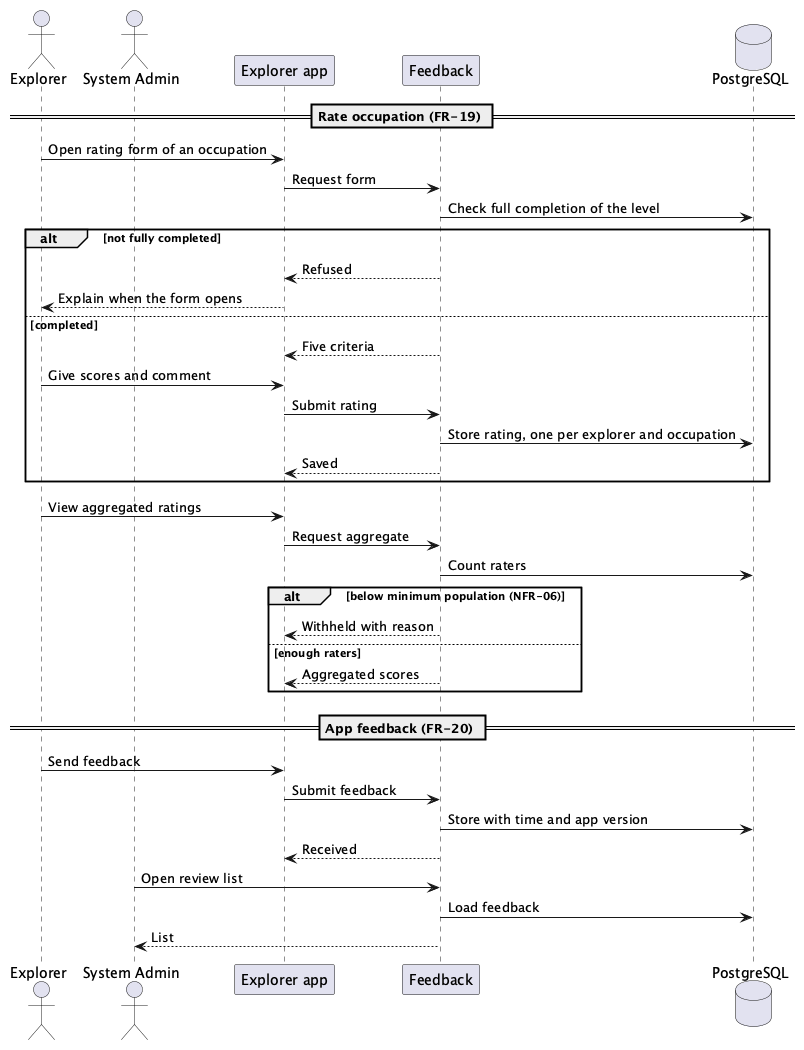
\includegraphics[width=\textwidth,height=0.9\textheight,keepaspectratio]{figures/SD-11_Explorer_RateAndFeedback.png}
\caption{Sequence of rating an occupation and sending app feedback (SD-11), with the administrator's review}
\end{figure}

\begin{figure}[H]
\centering
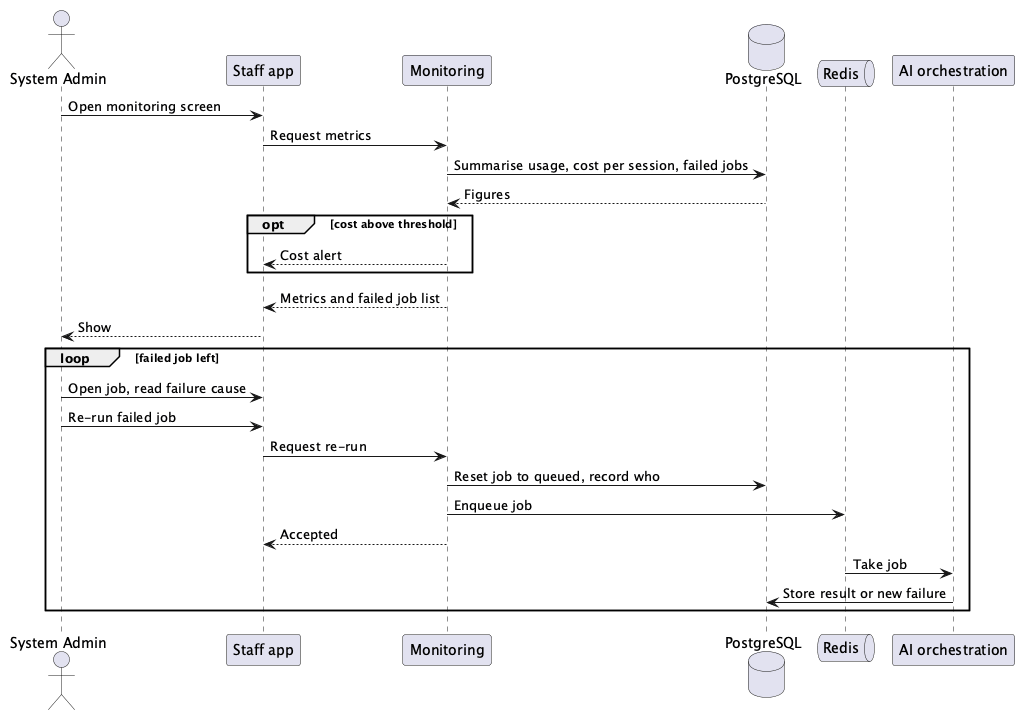
\includegraphics[width=\textwidth,height=0.9\textheight,keepaspectratio]{figures/SD-12_SystemAdmin_MonitorAndRerun.png}
\caption{Sequence of monitoring operation and re-running a failed job (SD-12)}
\end{figure}

\begin{figure}[H]
\centering
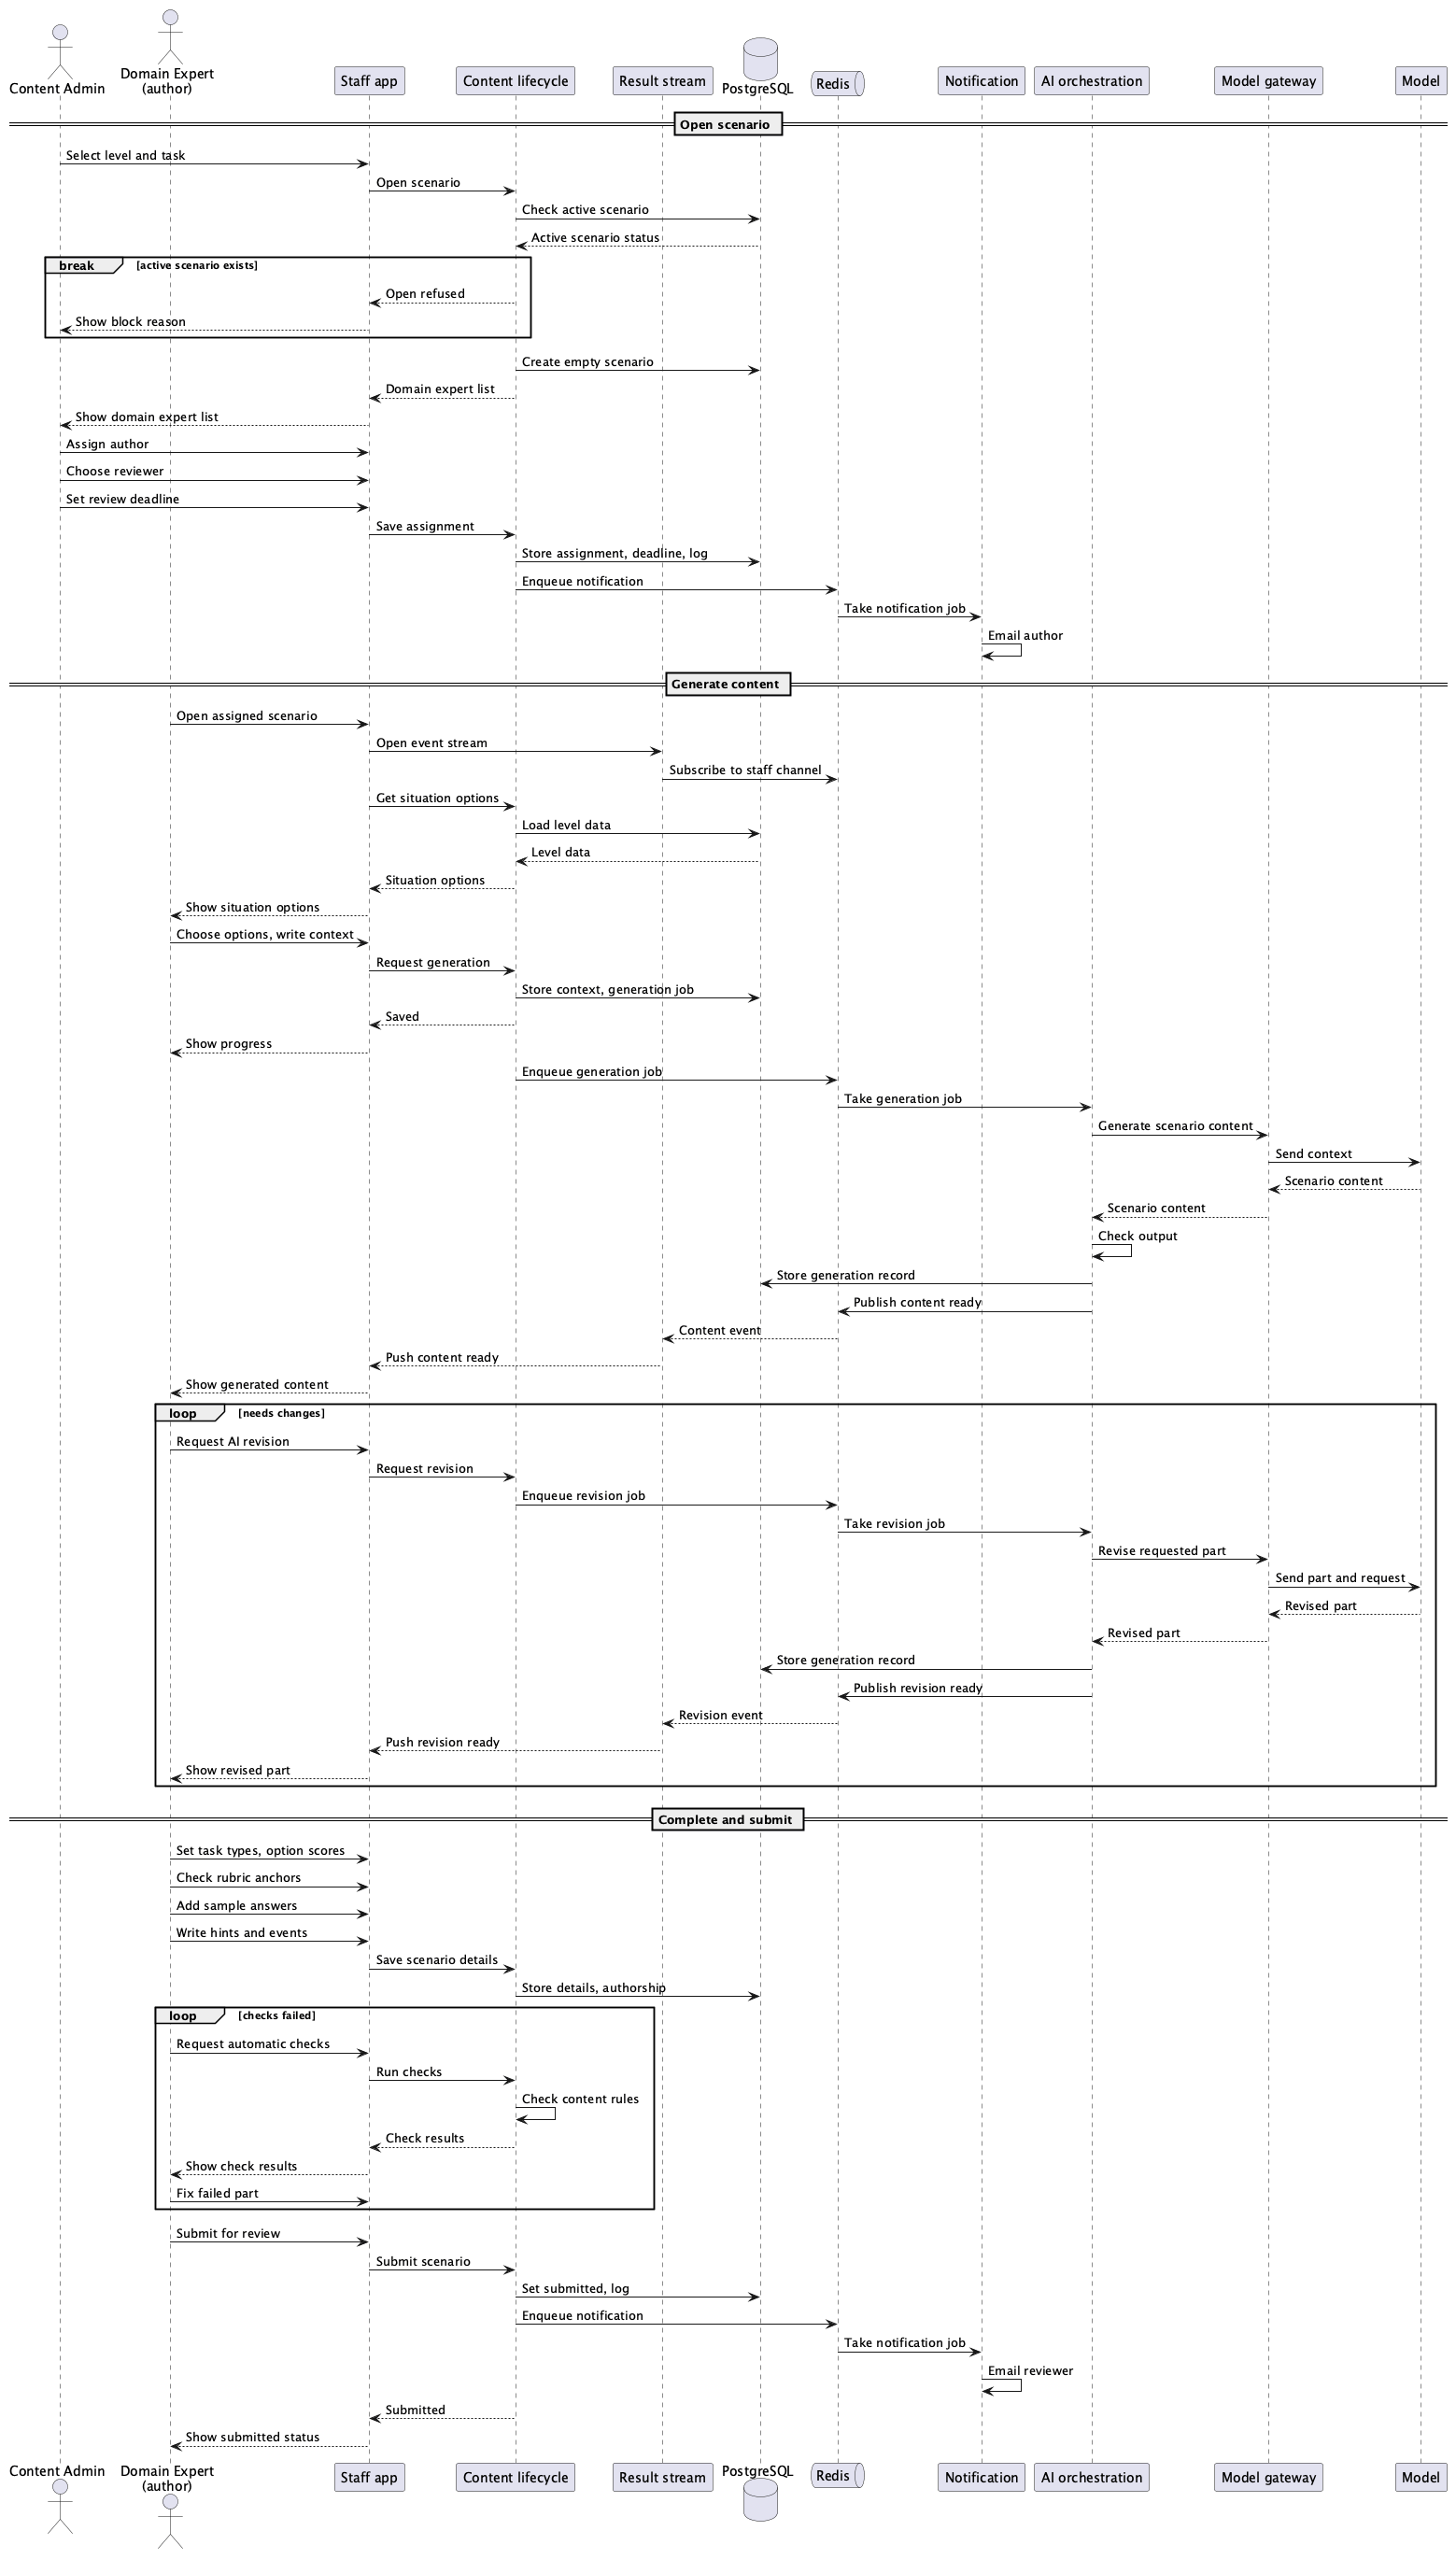
\includegraphics[width=\textwidth,height=0.9\textheight,keepaspectratio]{figures/SD-05_DomainExpert_GenerateScenario.png}
\caption{Sequence of generating scenario content (SD-05): opening and assignment, generation and revision with AI, and completion and submission}
\end{figure}

Module classes. An association is constructor injection, a dashed arrow labelled «write» marks a table the module owns, and a dashed arrow with a hollow head is a realization.

\begin{landscape}
\begin{figure}[H]
\centering
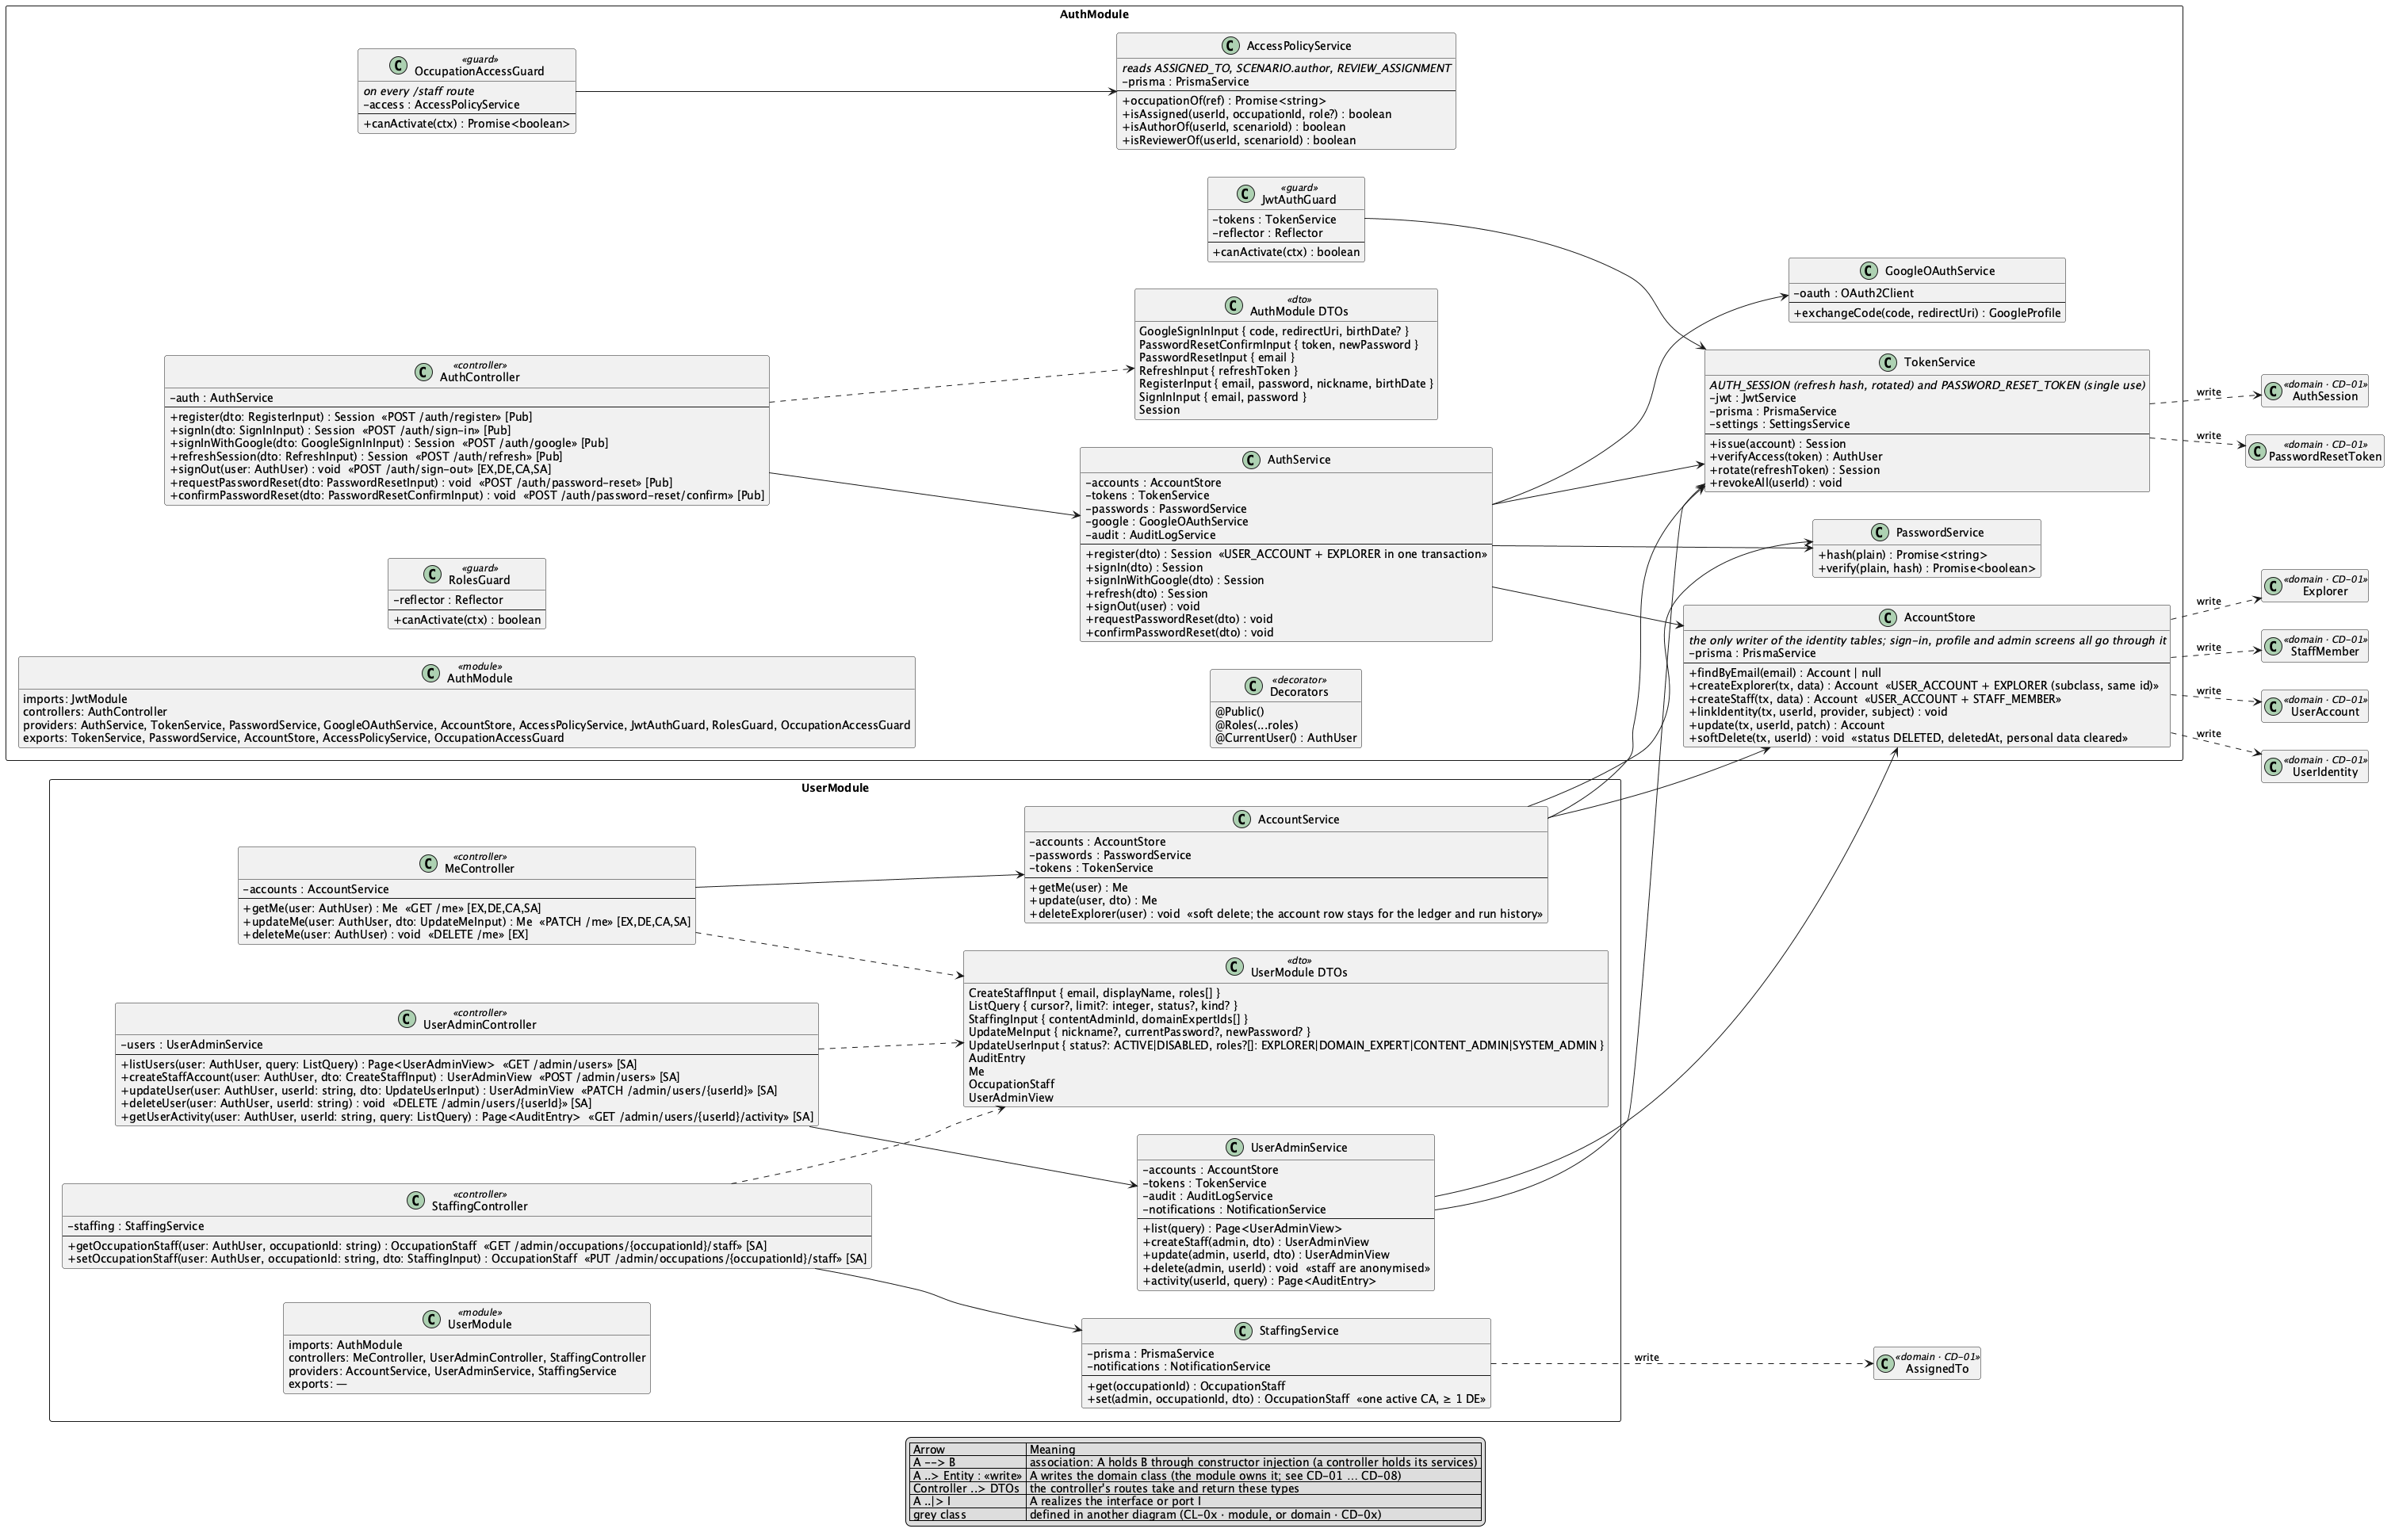
\includegraphics[width=\linewidth,height=0.86\textwidth,keepaspectratio,keepaspectratio]{figures/CL-01_IdentityAndAccess.png}
\caption{Module classes of identity and access (CL-01)}
\end{figure}
\end{landscape}

\begin{landscape}
\begin{figure}[H]
\centering
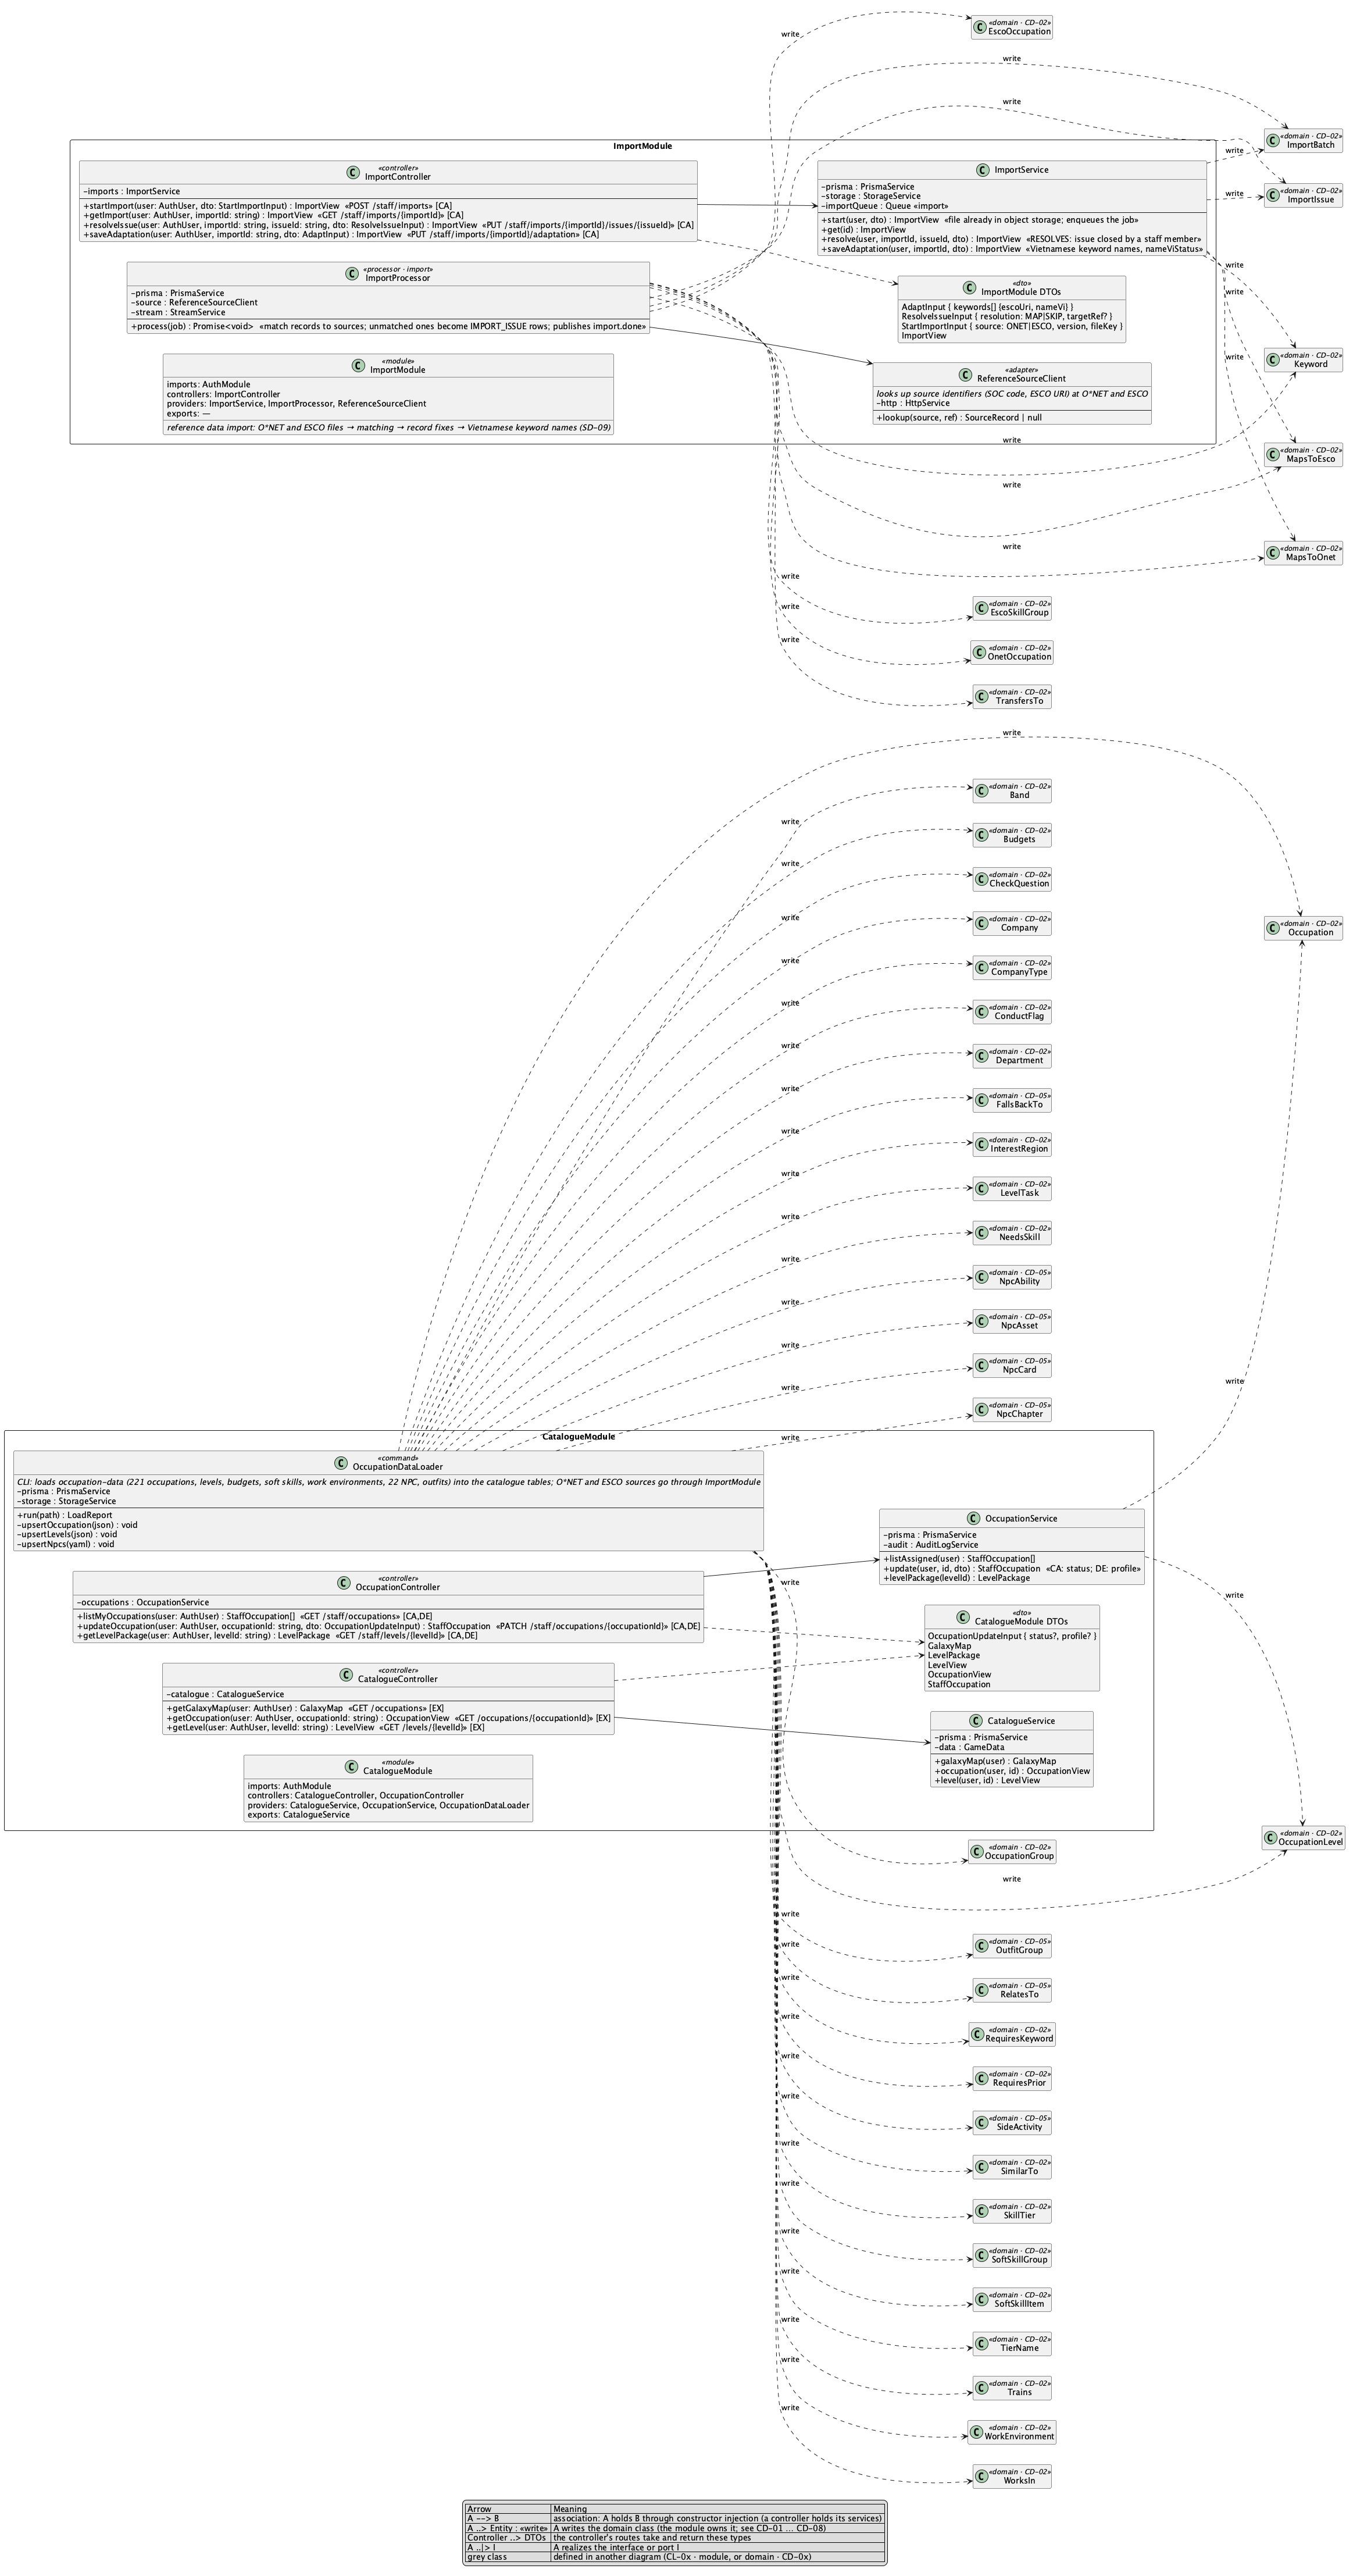
\includegraphics[width=\linewidth,height=0.86\textwidth,keepaspectratio,keepaspectratio]{figures/CL-02_CatalogueAndImport.png}
\caption{Module classes of the catalogue and import (CL-02)}
\end{figure}
\end{landscape}

\begin{landscape}
\begin{figure}[H]
\centering
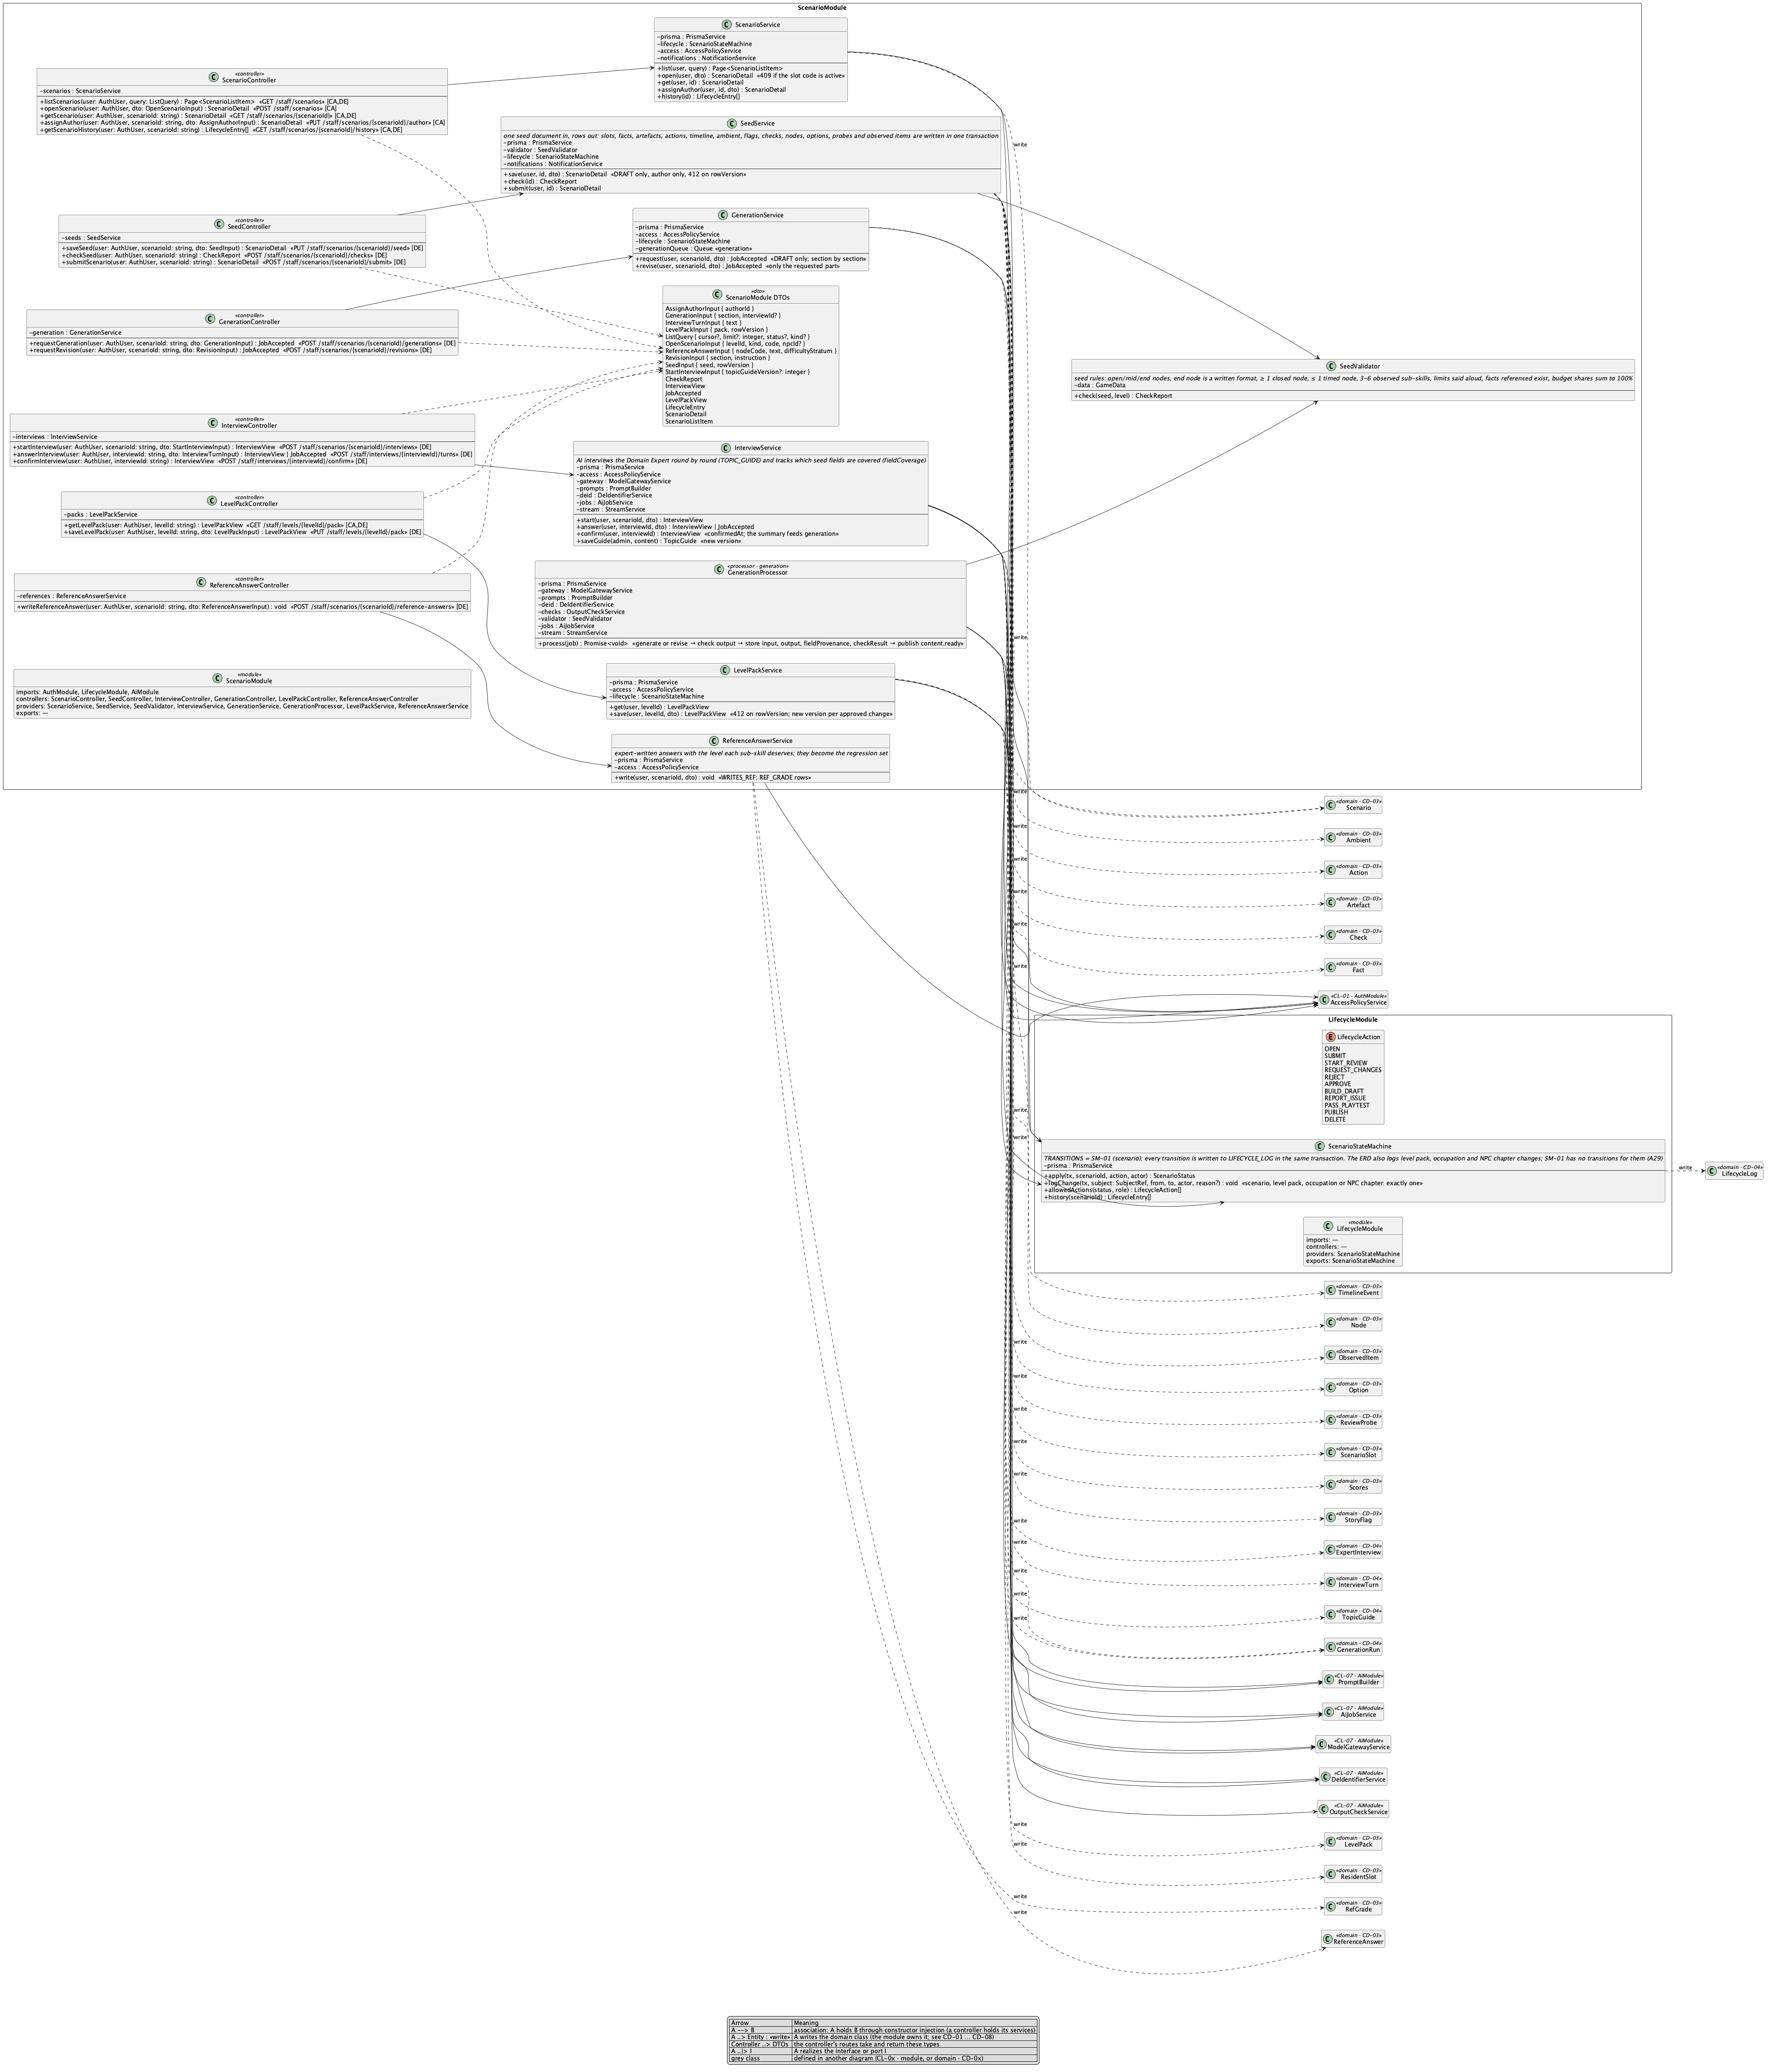
\includegraphics[width=\linewidth,height=0.86\textwidth,keepaspectratio,keepaspectratio]{figures/CL-03_ScenarioAuthoringAndLifecycle.png}
\caption{Module classes of scenario authoring and lifecycle (CL-03)}
\end{figure}
\end{landscape}

\begin{landscape}
\begin{figure}[H]
\centering
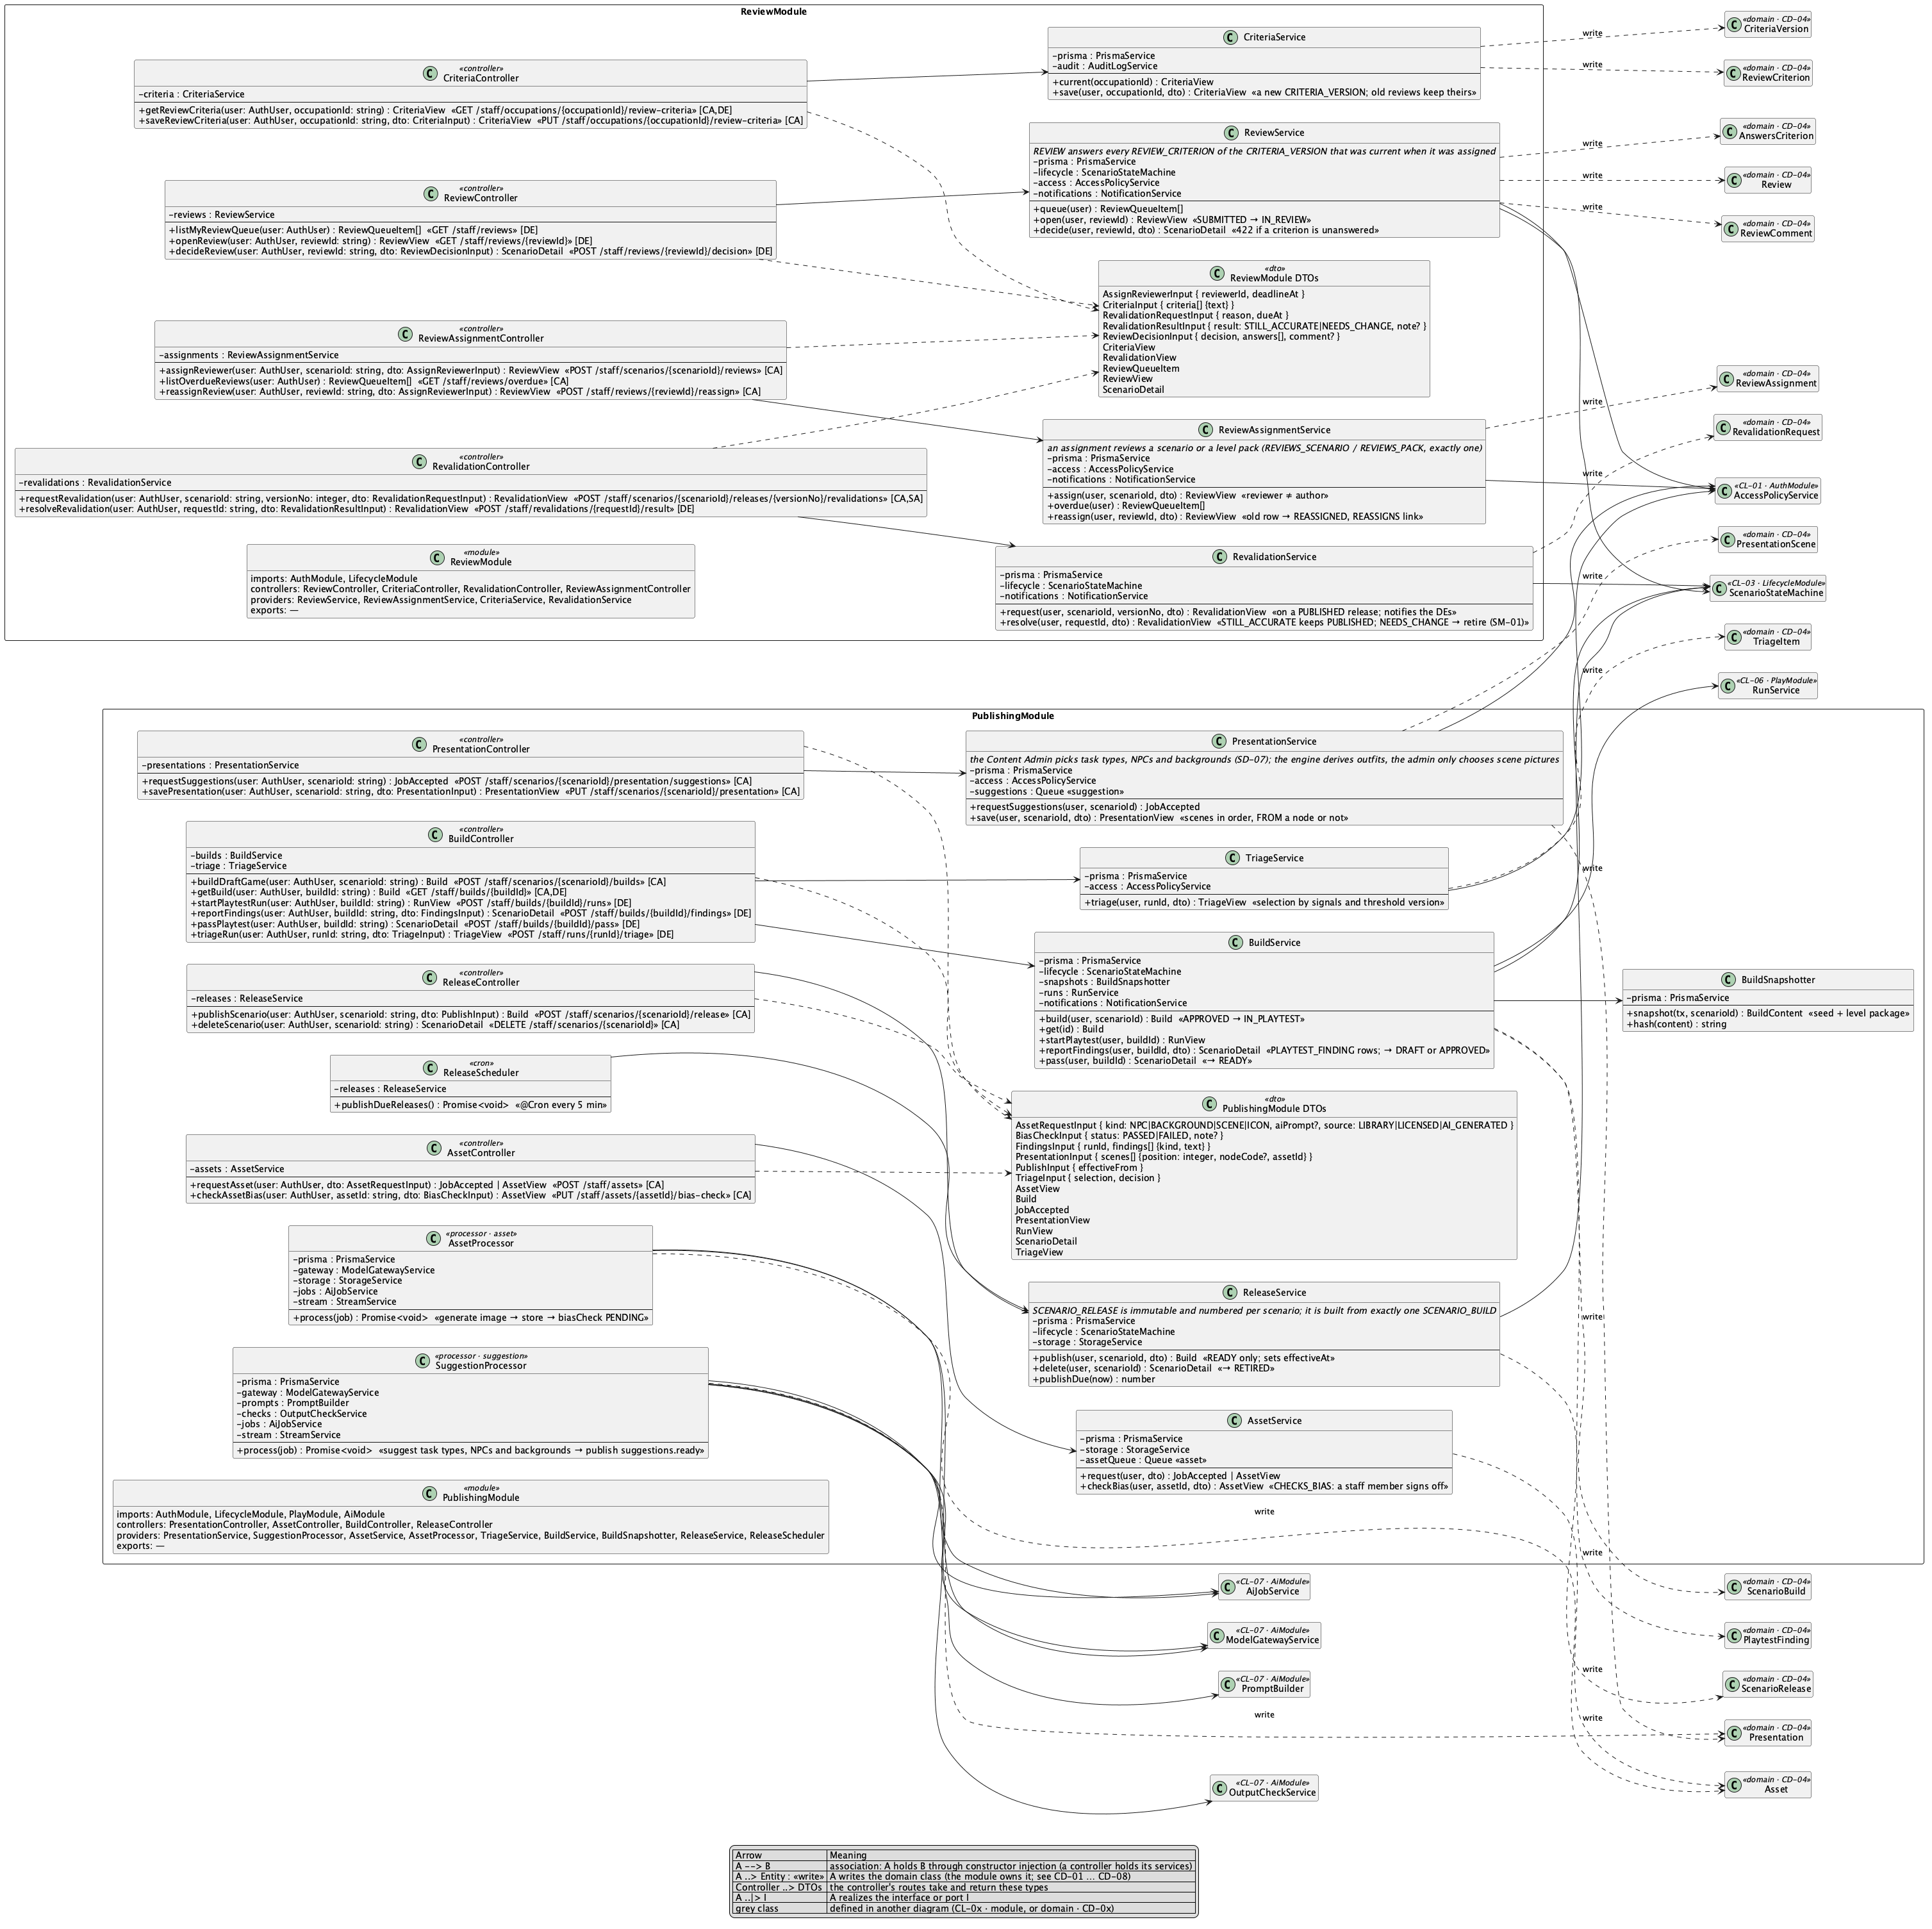
\includegraphics[width=\linewidth,height=0.86\textwidth,keepaspectratio,keepaspectratio]{figures/CL-04_ReviewAndPublishing.png}
\caption{Module classes of review and publishing (CL-04)}
\end{figure}
\end{landscape}

\begin{landscape}
\begin{figure}[H]
\centering
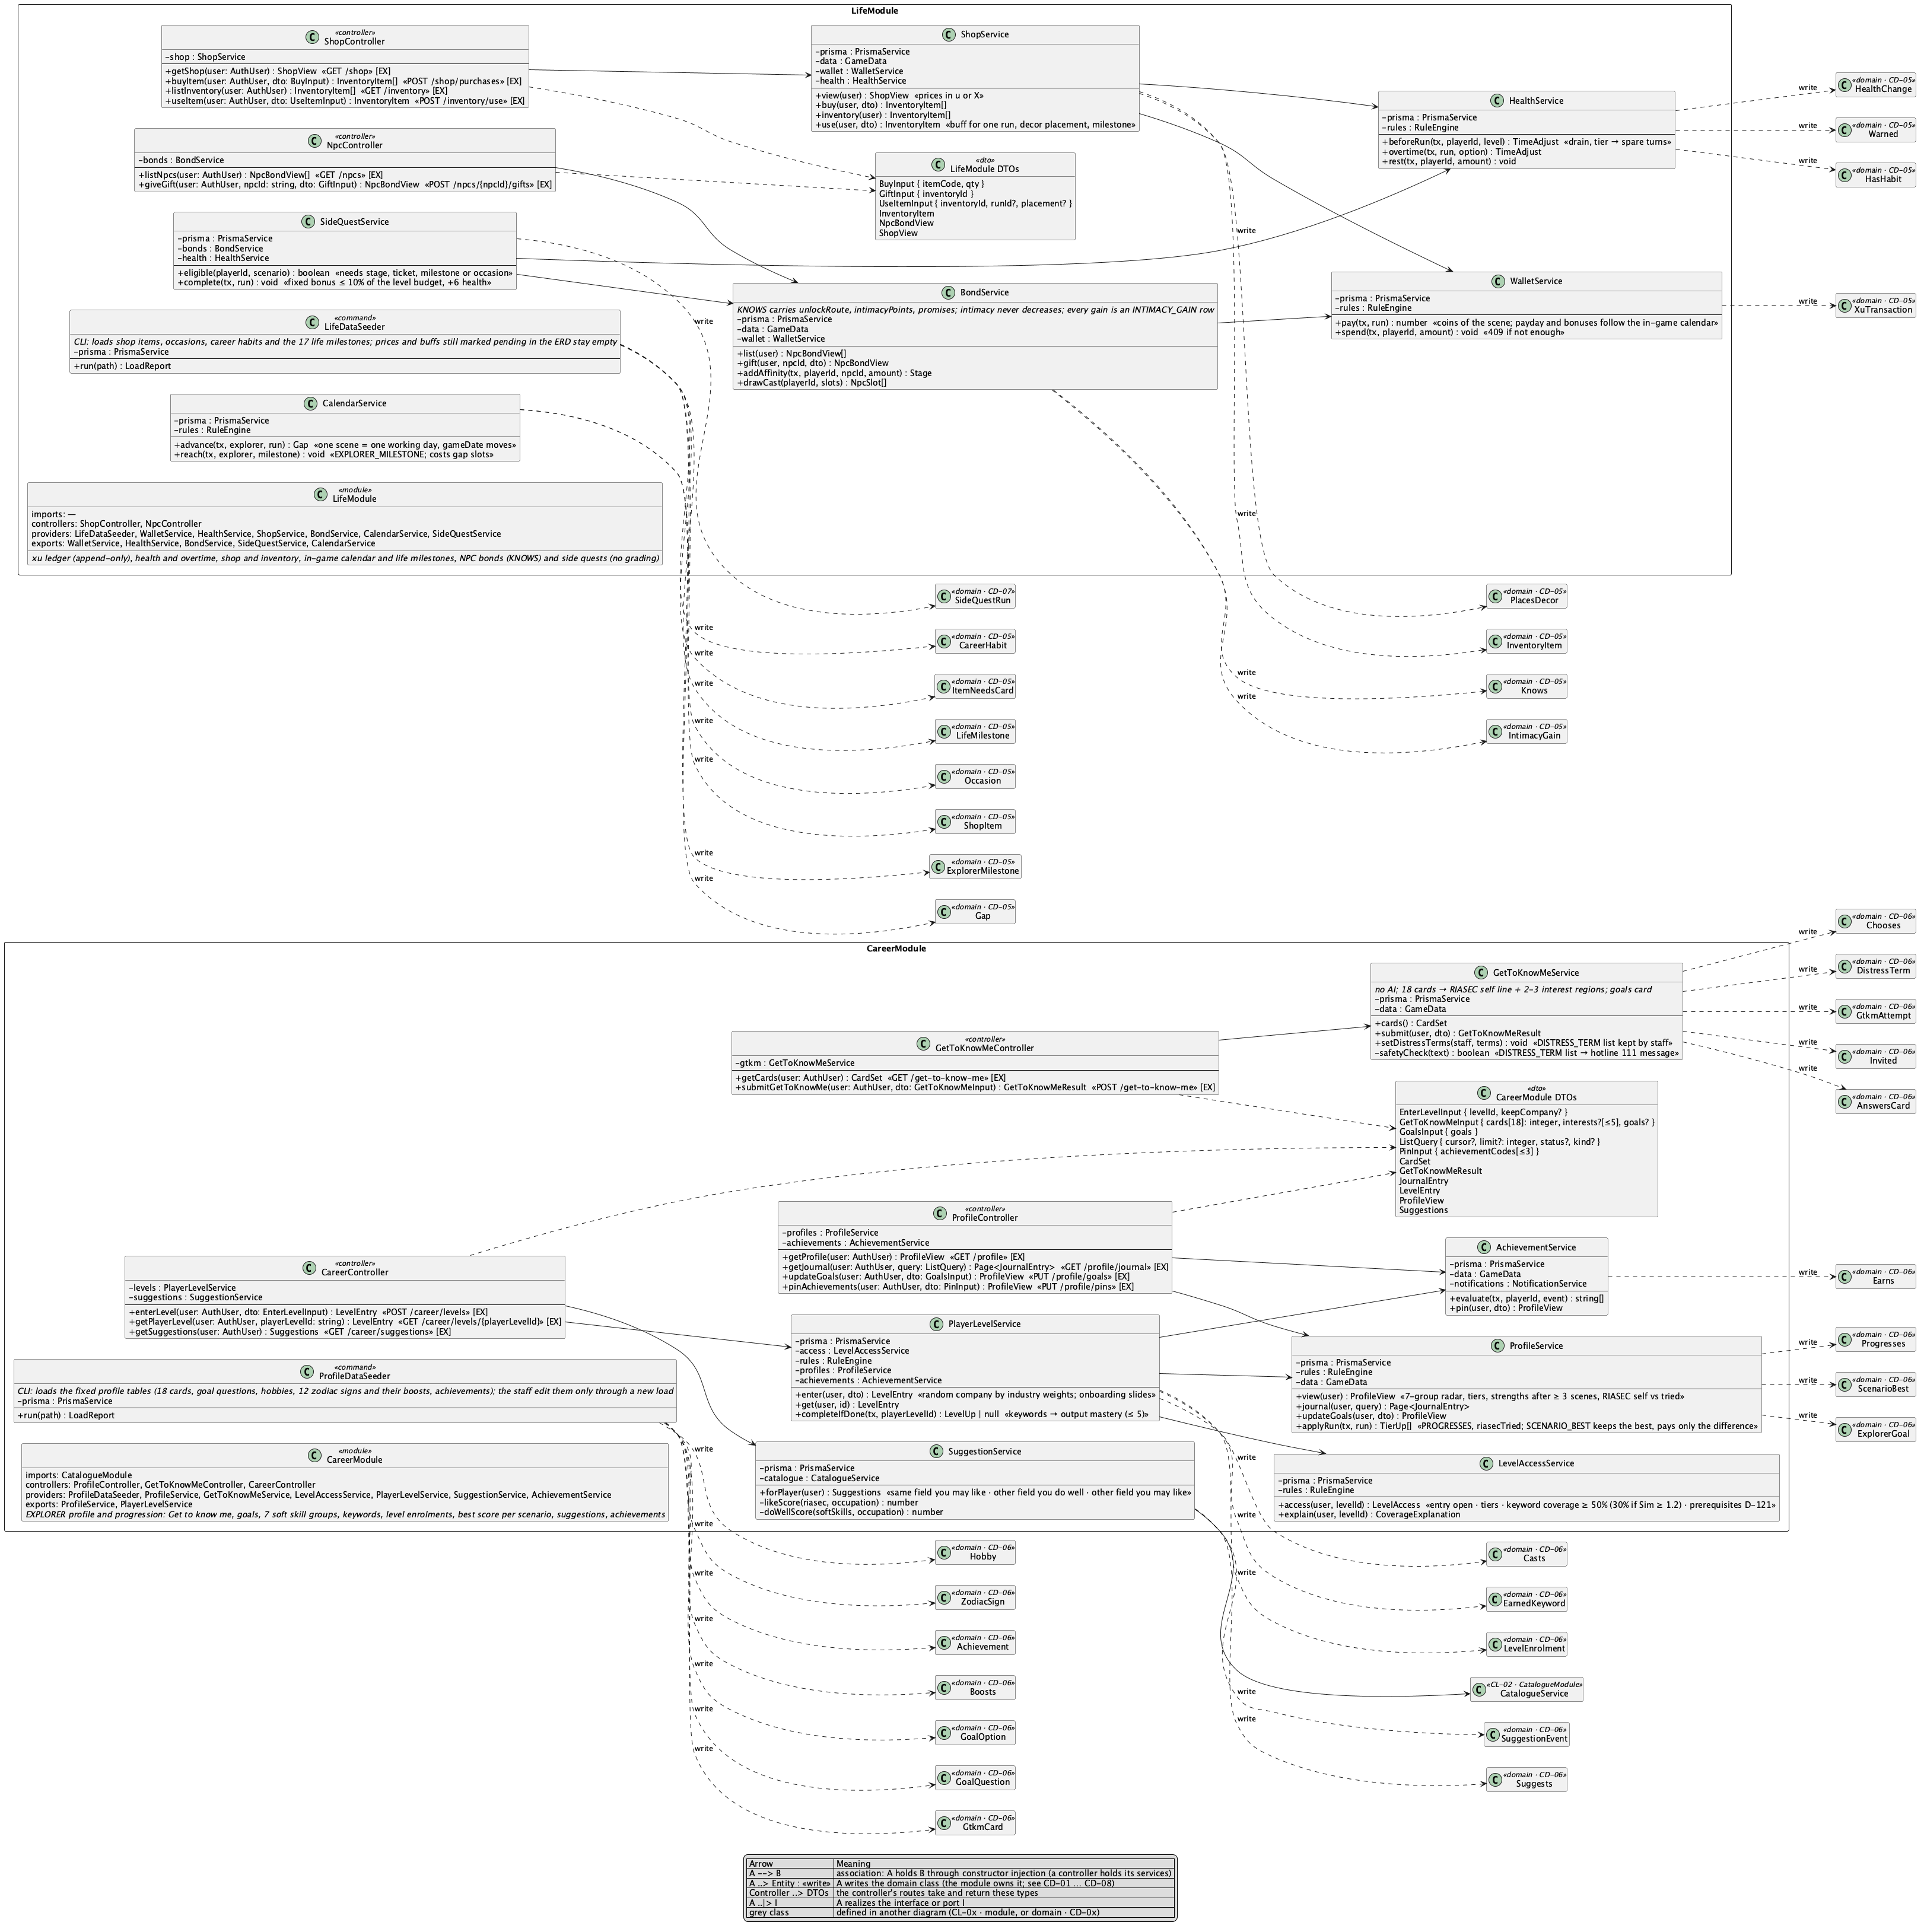
\includegraphics[width=\linewidth,height=0.86\textwidth,keepaspectratio,keepaspectratio]{figures/CL-05_ExplorerCareerAndLife.png}
\caption{Module classes of the explorer, career, and life (CL-05)}
\end{figure}
\end{landscape}

\begin{landscape}
\begin{figure}[H]
\centering
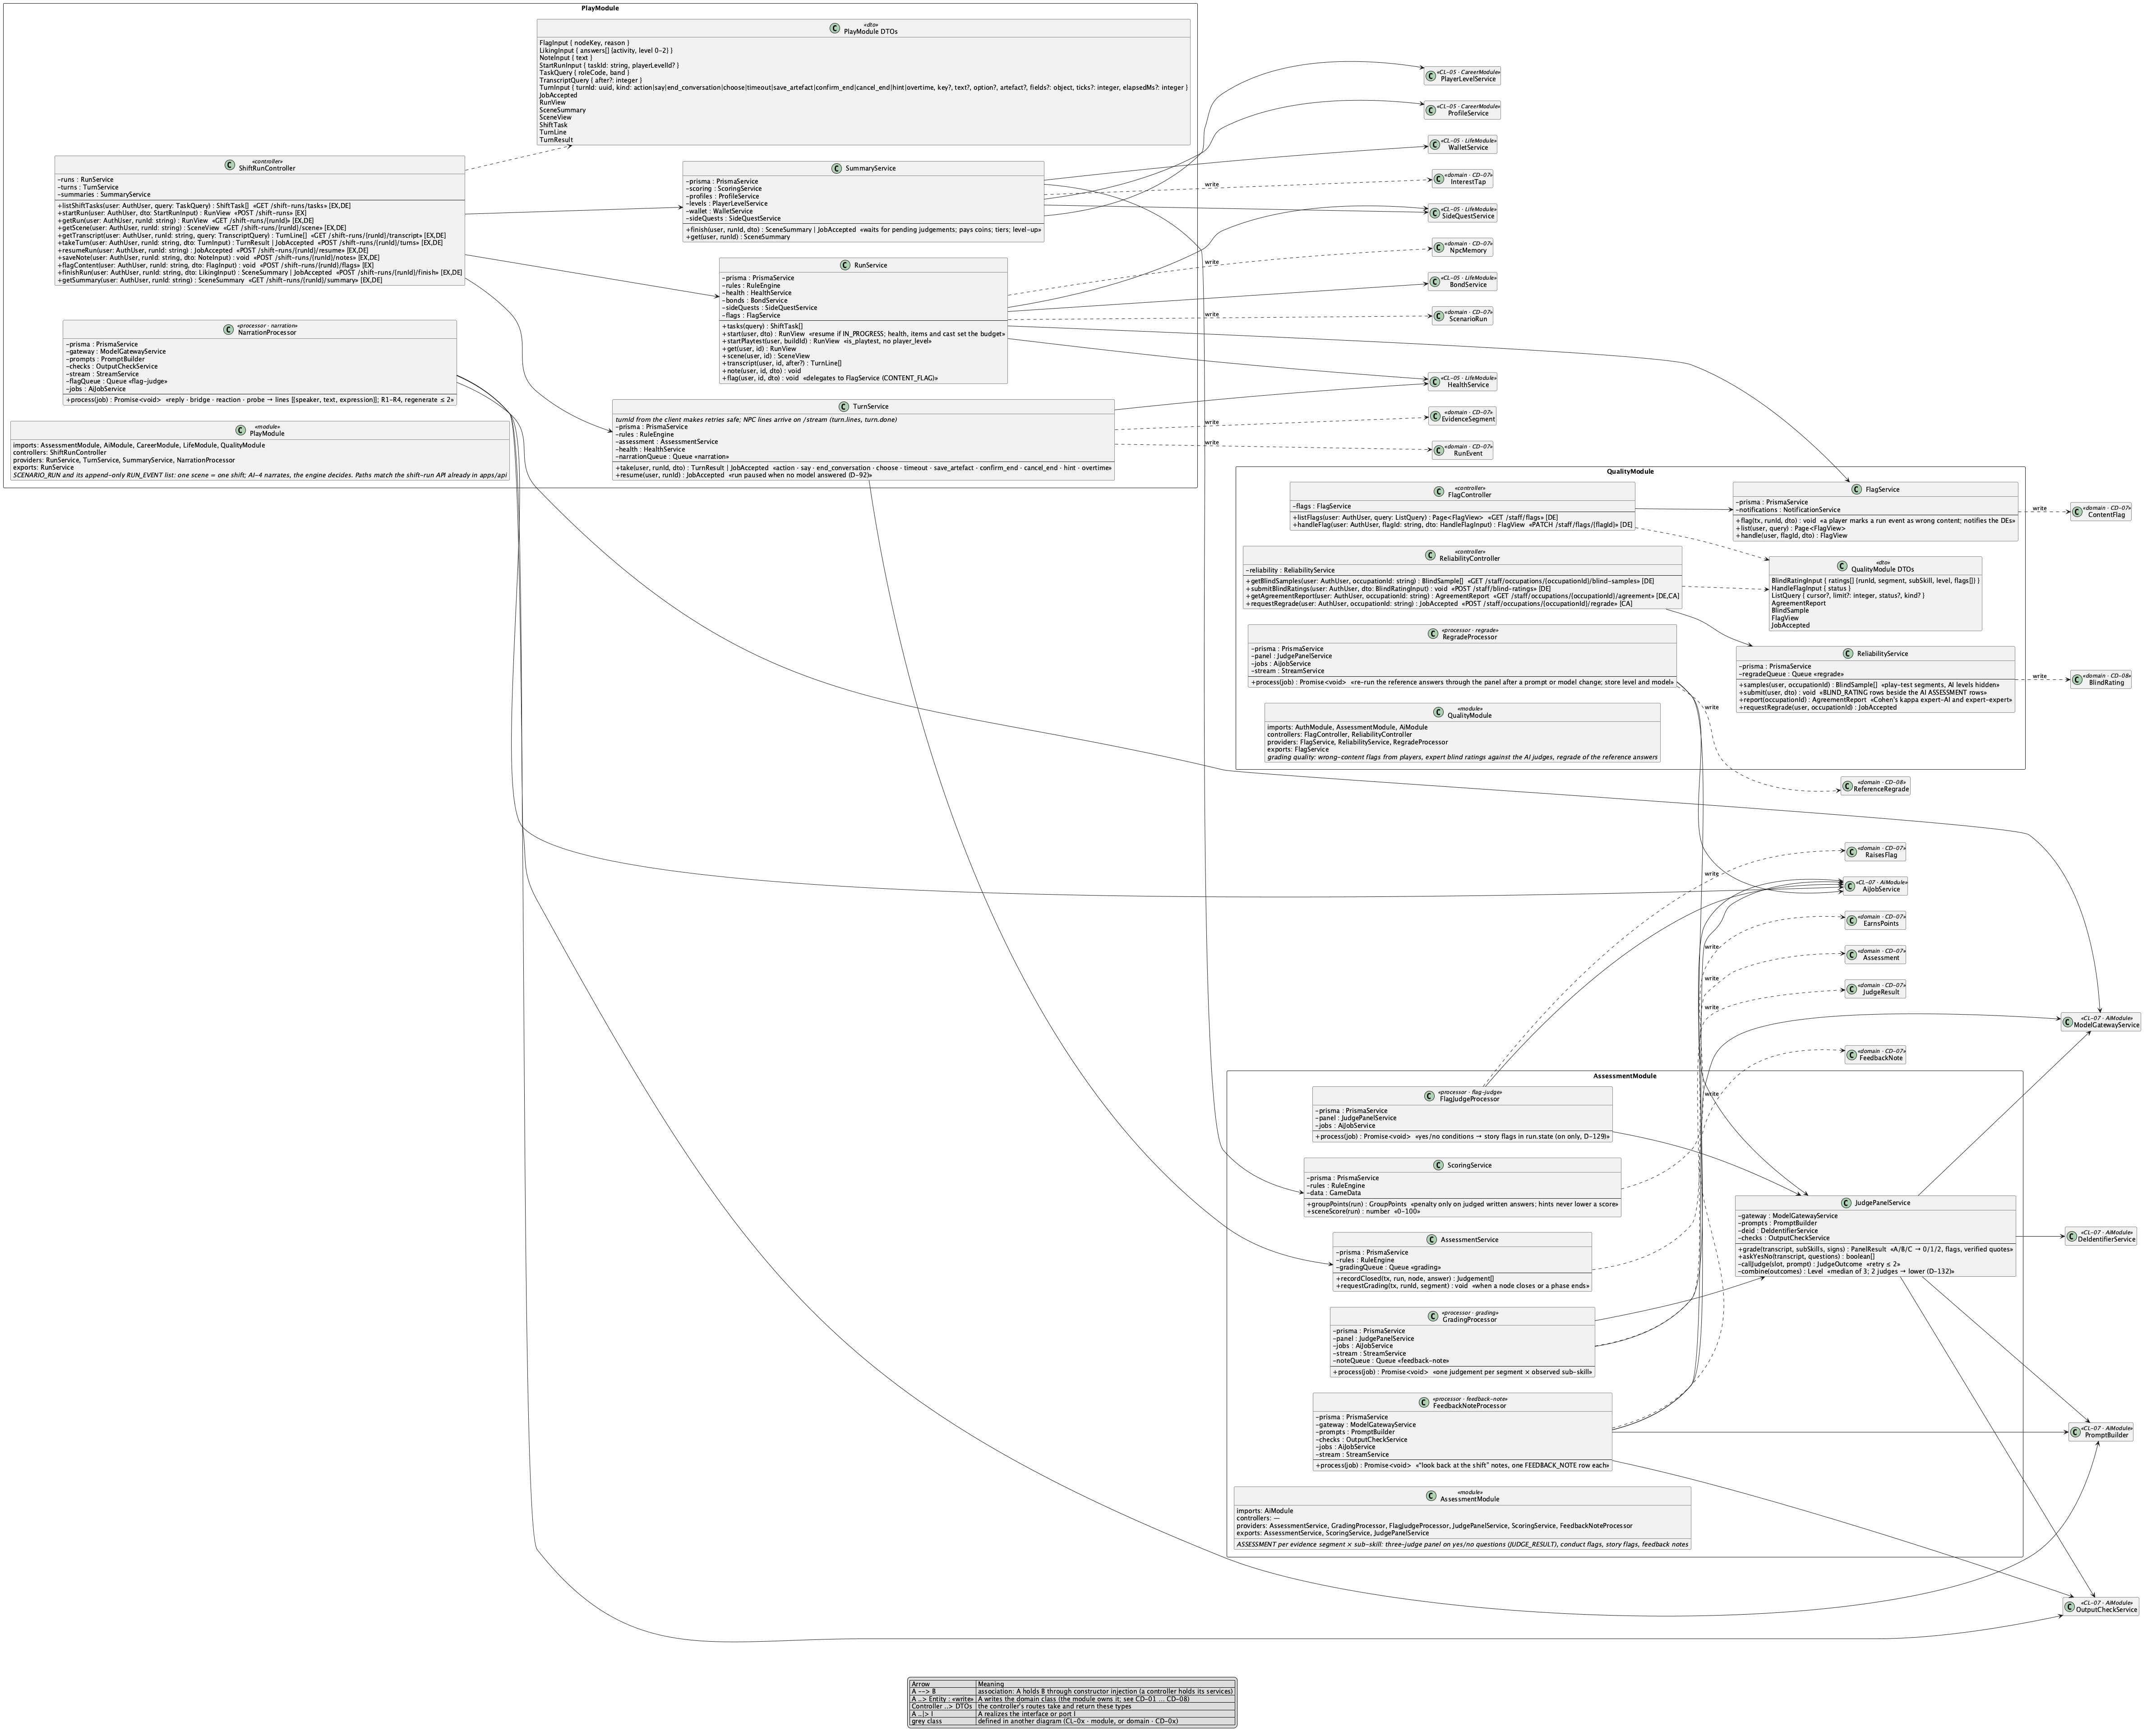
\includegraphics[width=\linewidth,height=0.86\textwidth,keepaspectratio,keepaspectratio]{figures/CL-06_PlayAssessmentAndQuality.png}
\caption{Module classes of play, assessment, and quality (CL-06)}
\end{figure}
\end{landscape}

\begin{landscape}
\begin{figure}[H]
\centering
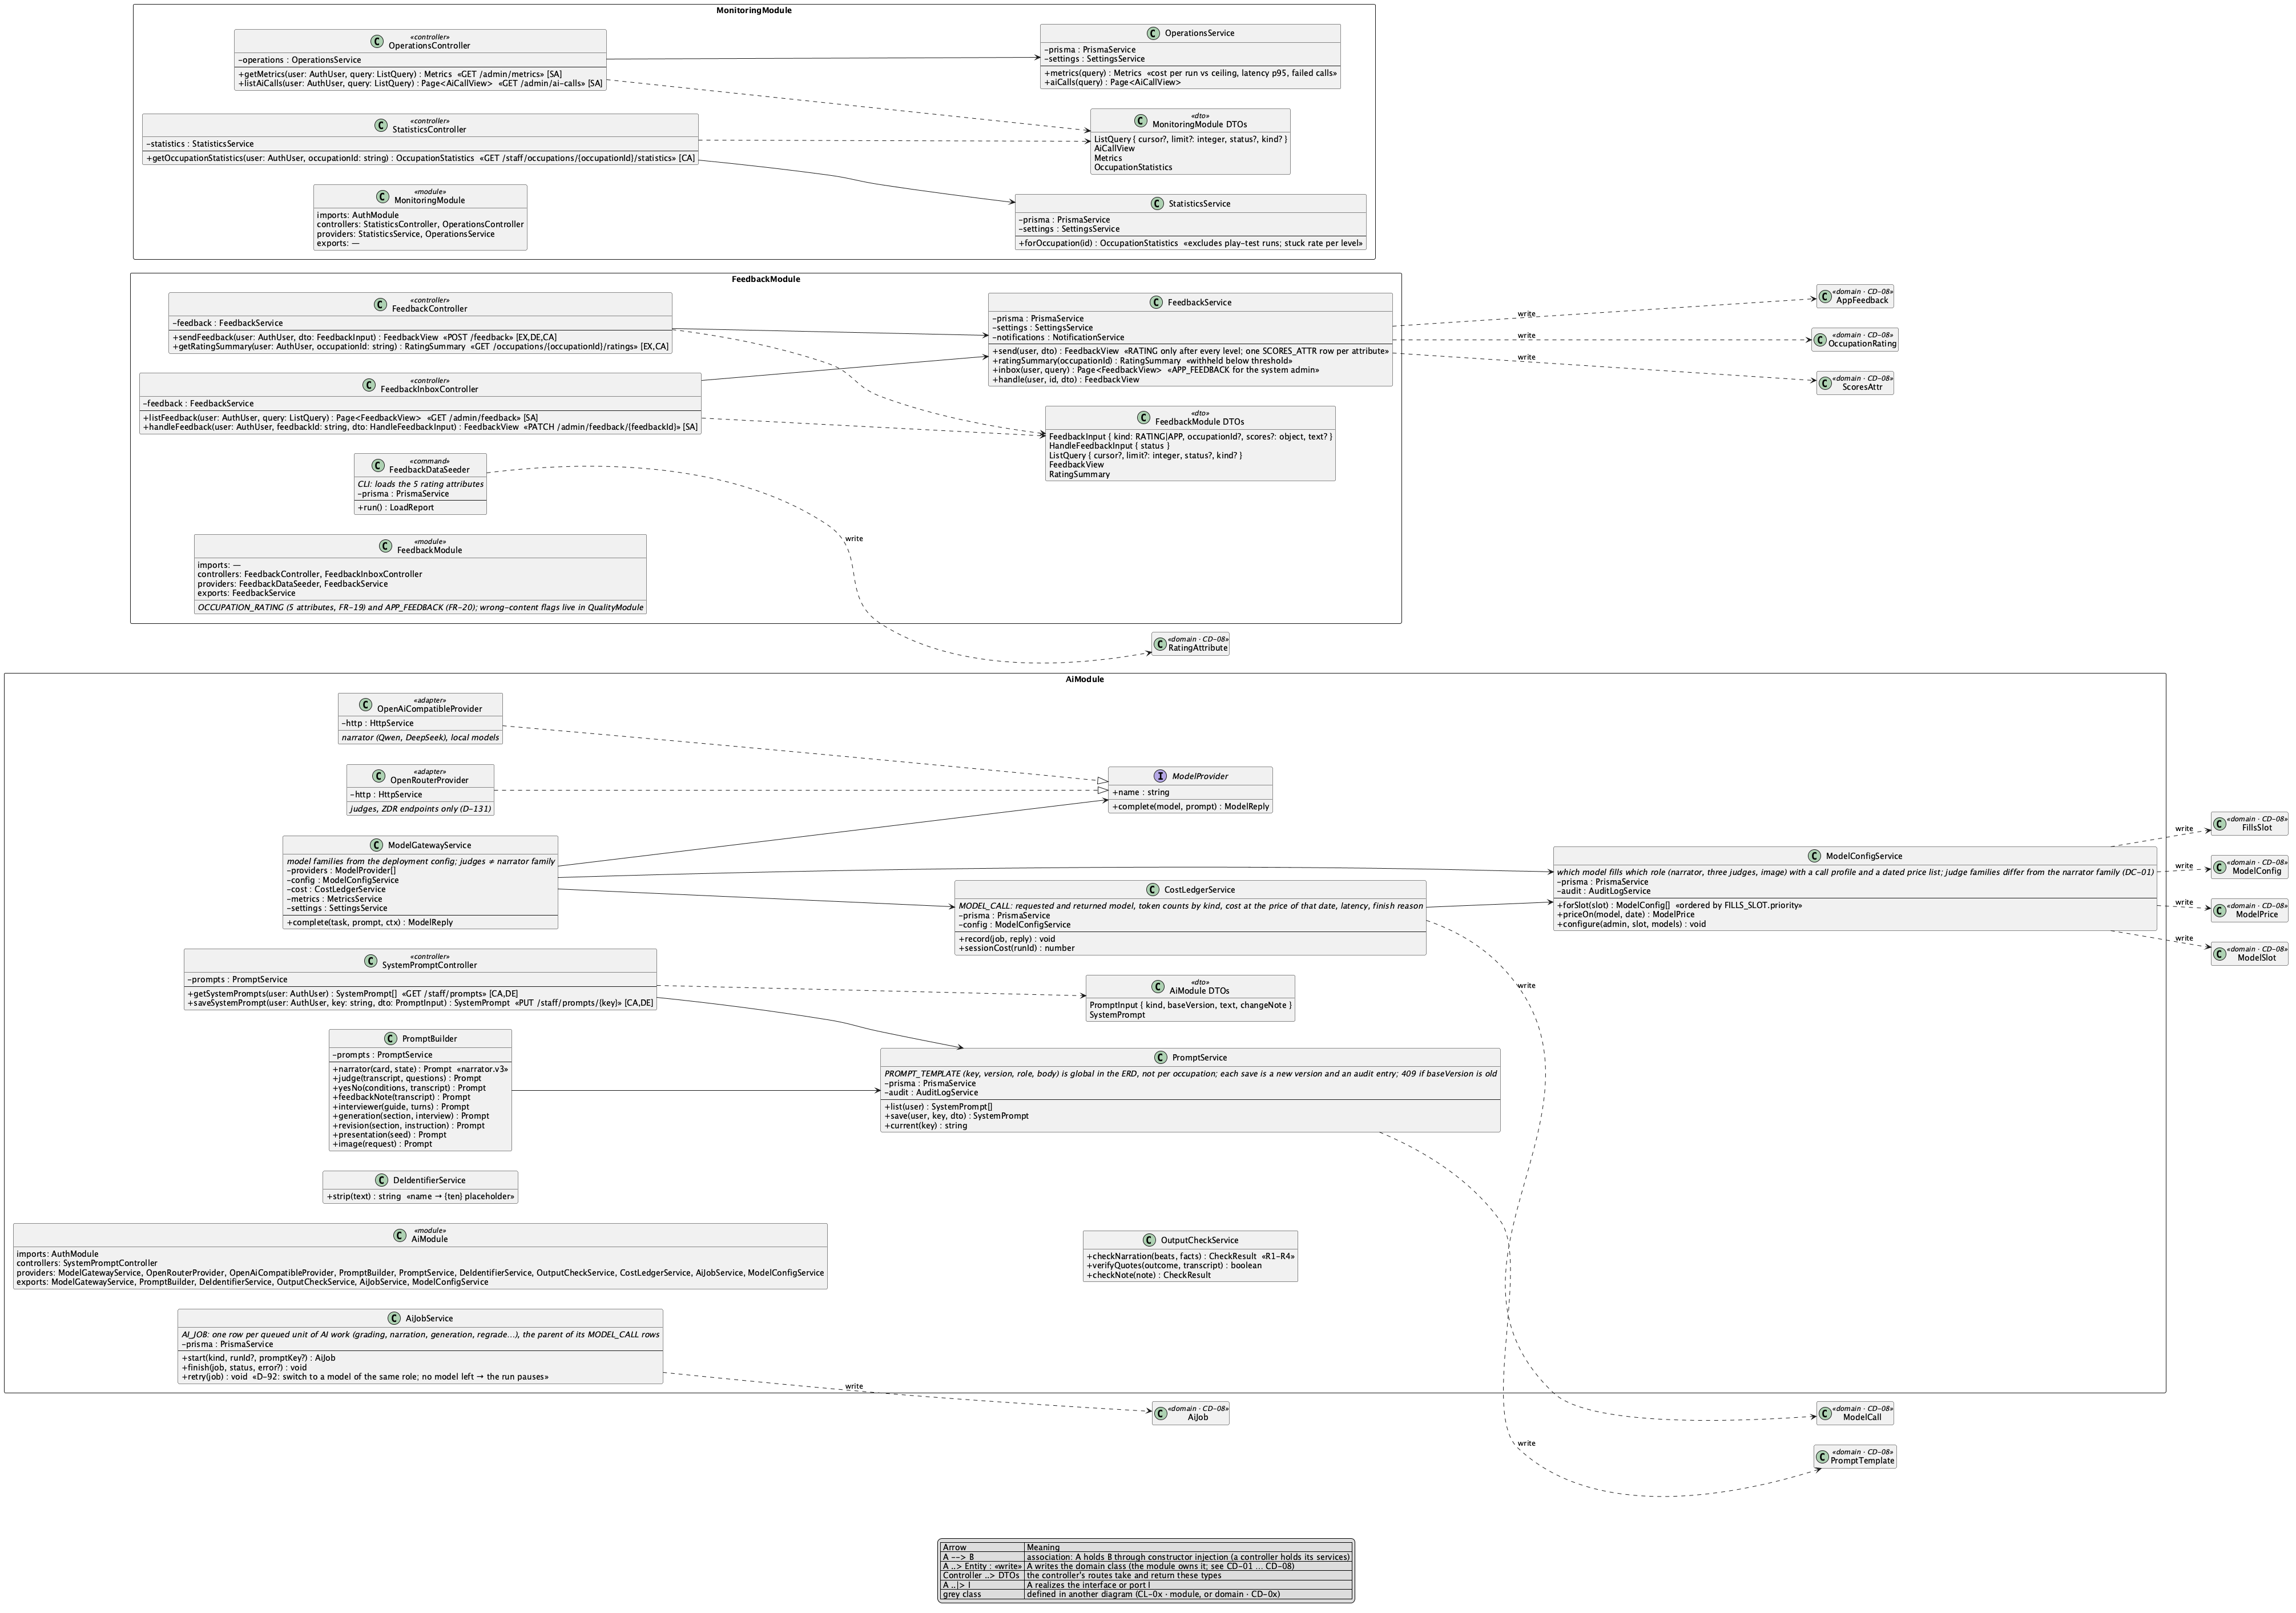
\includegraphics[width=\linewidth,height=0.86\textwidth,keepaspectratio,keepaspectratio]{figures/CL-07_AiFeedbackAndMonitoring.png}
\caption{Module classes of AI, feedback, and monitoring (CL-07)}
\end{figure}
\end{landscape}

\begin{landscape}
\begin{figure}[H]
\centering
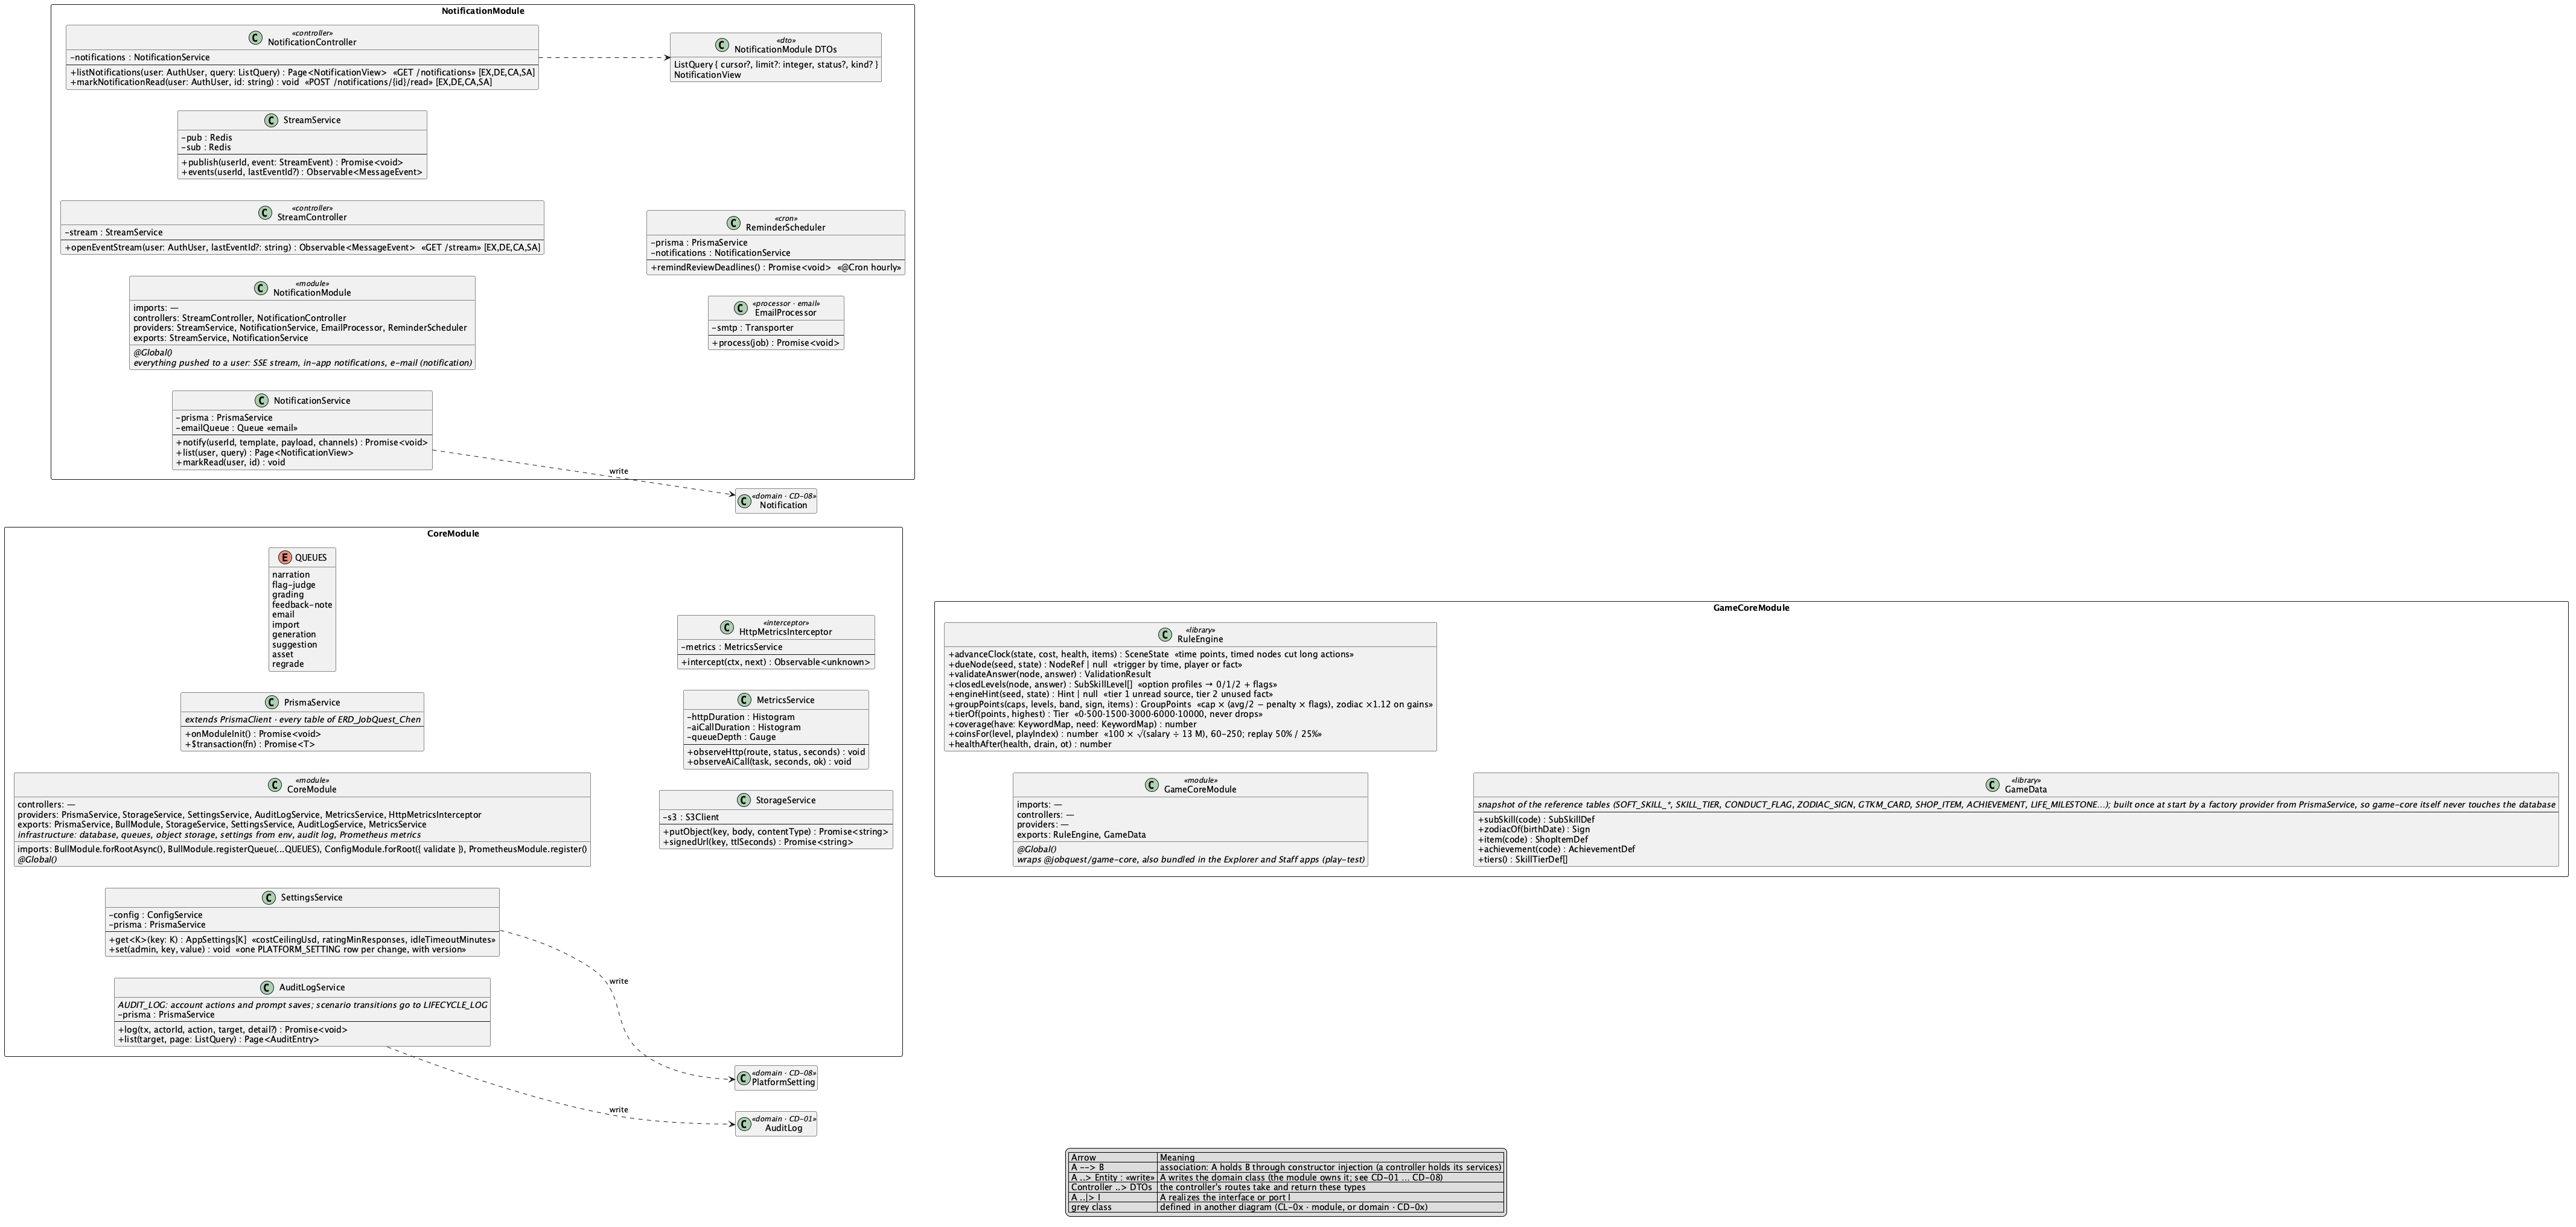
\includegraphics[width=\linewidth,height=0.86\textwidth,keepaspectratio,keepaspectratio]{figures/CL-08_SharedPlatform.png}
\caption{Module classes of the shared platform (CL-08)}
\end{figure}
\end{landscape}

Entity--relationship views.

\begin{figure}[H]
\centering
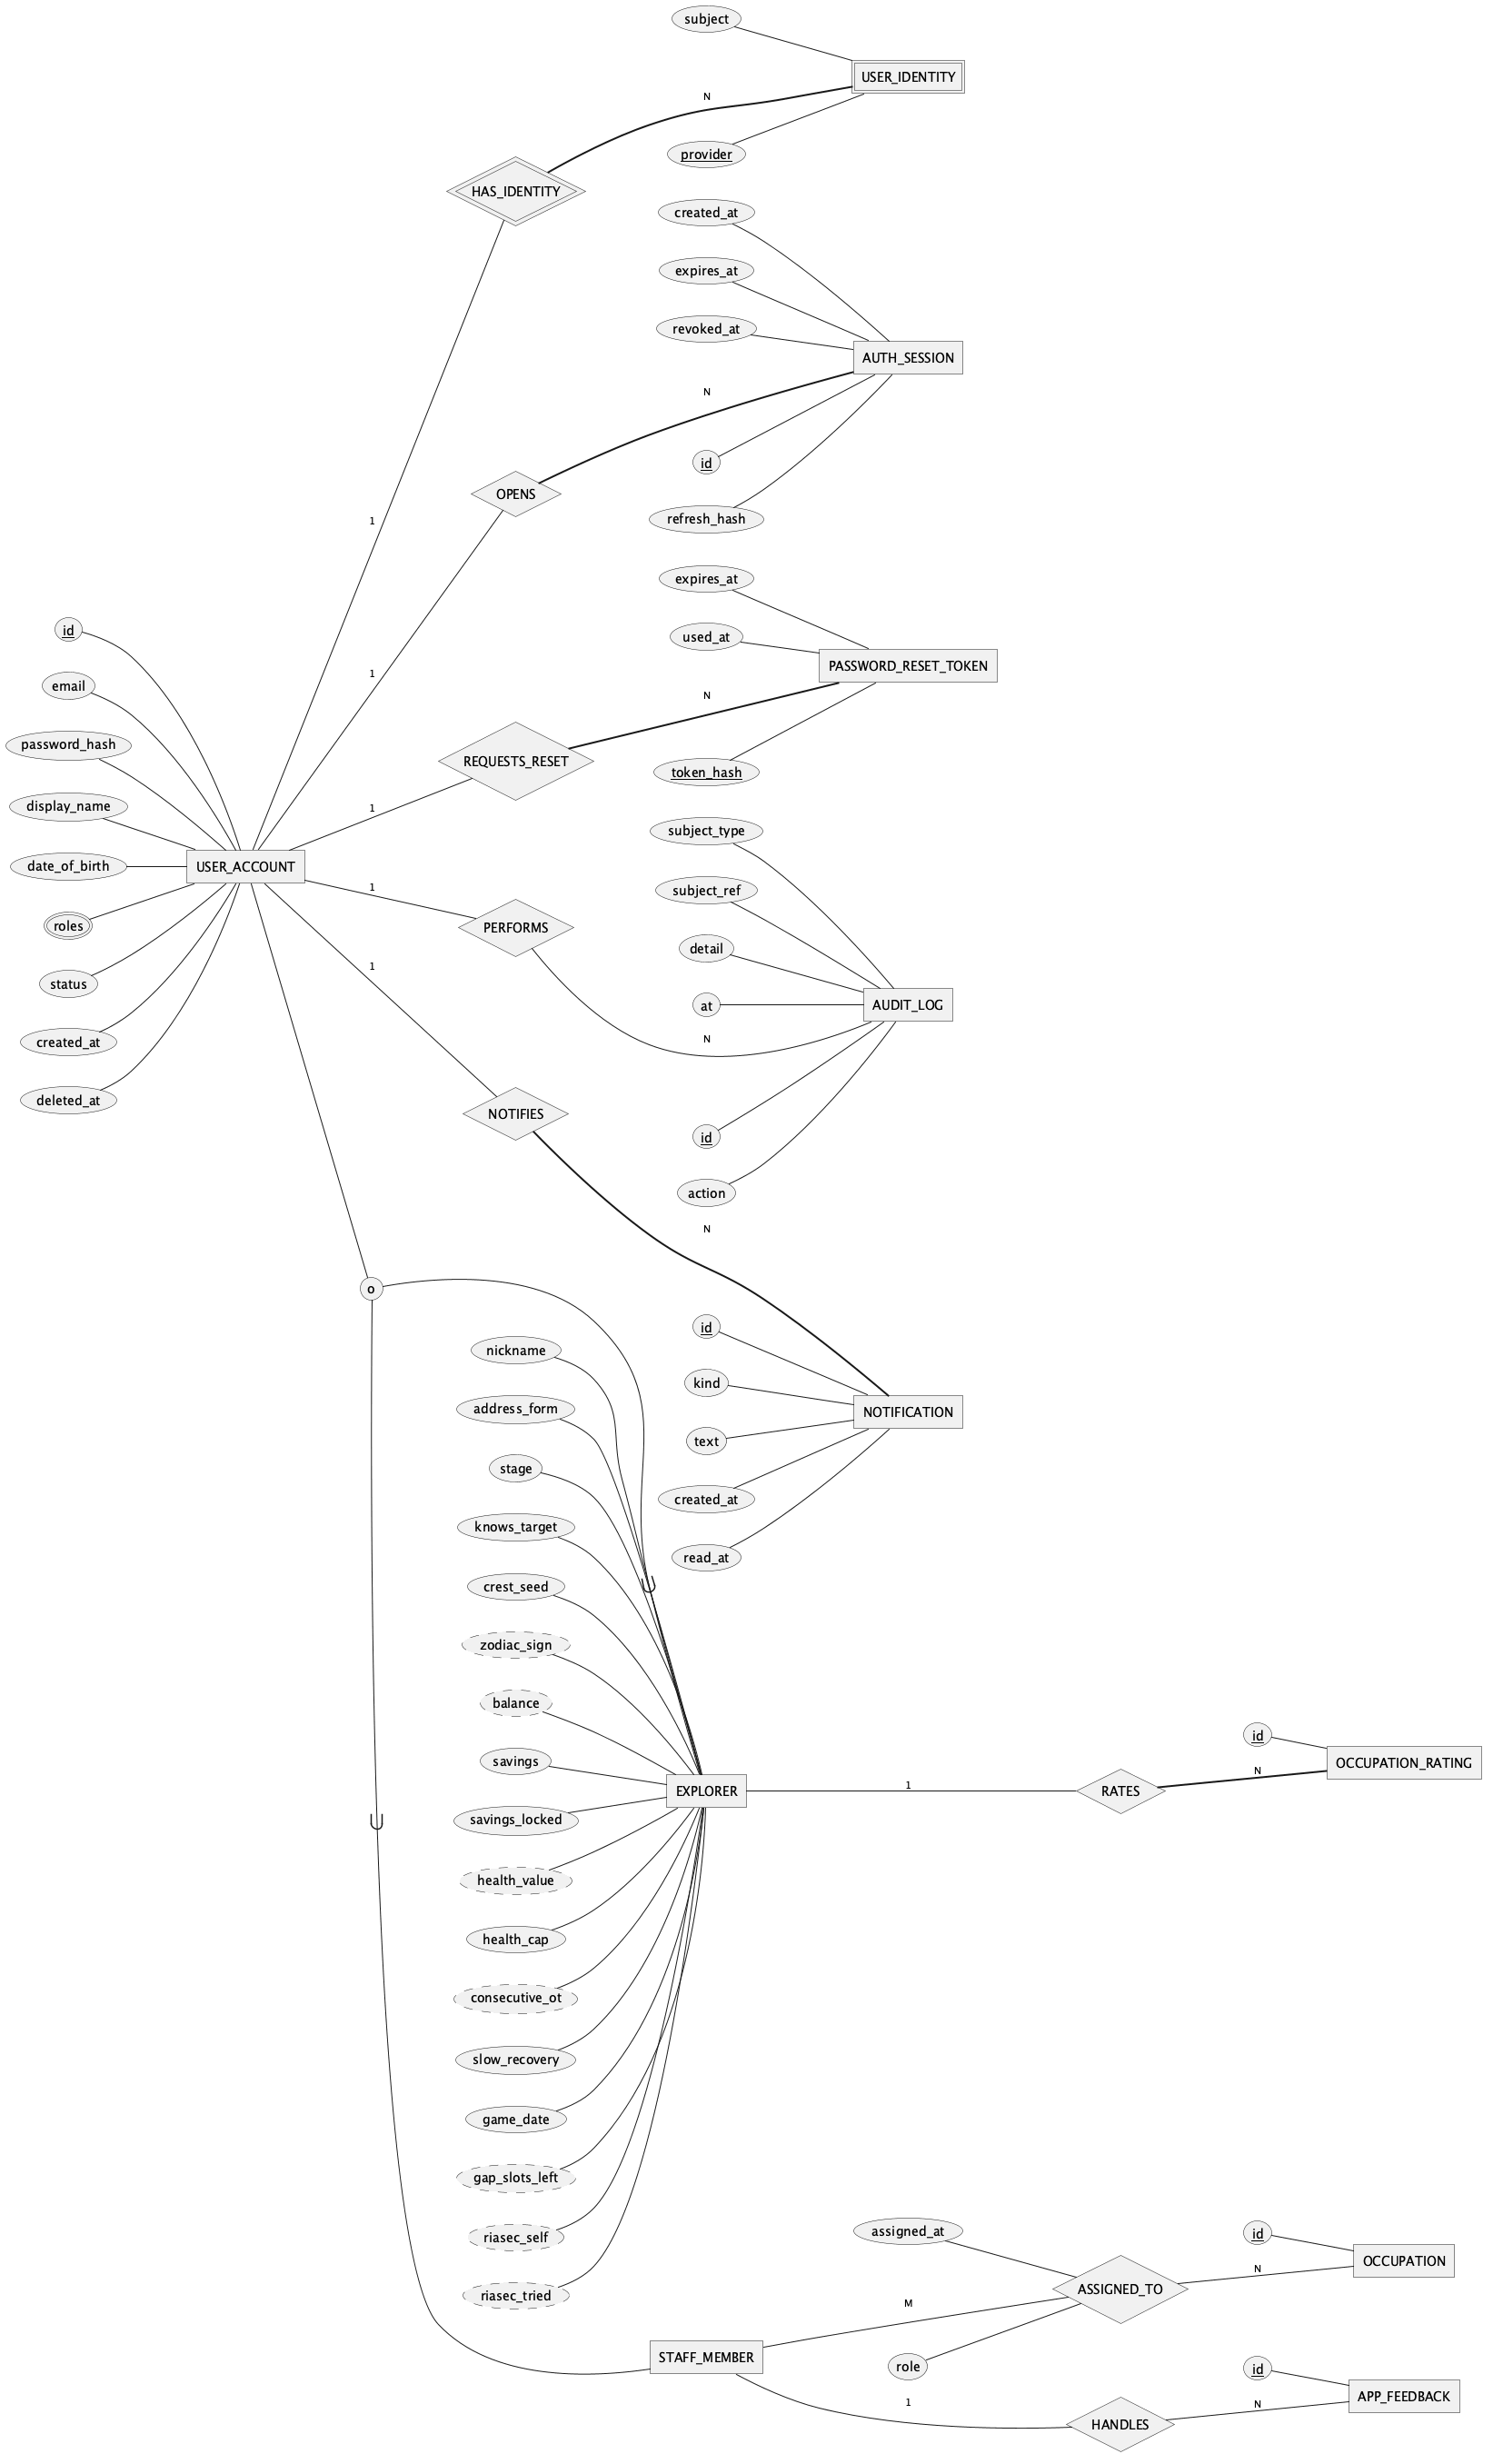
\includegraphics[width=\textwidth,height=0.9\textheight,keepaspectratio]{figures/ERD-01a_Identity.png}
\caption{Entity--relationship diagram ERD-01a: Identity and assignment}
\end{figure}

\begin{landscape}
\begin{figure}[H]
\centering
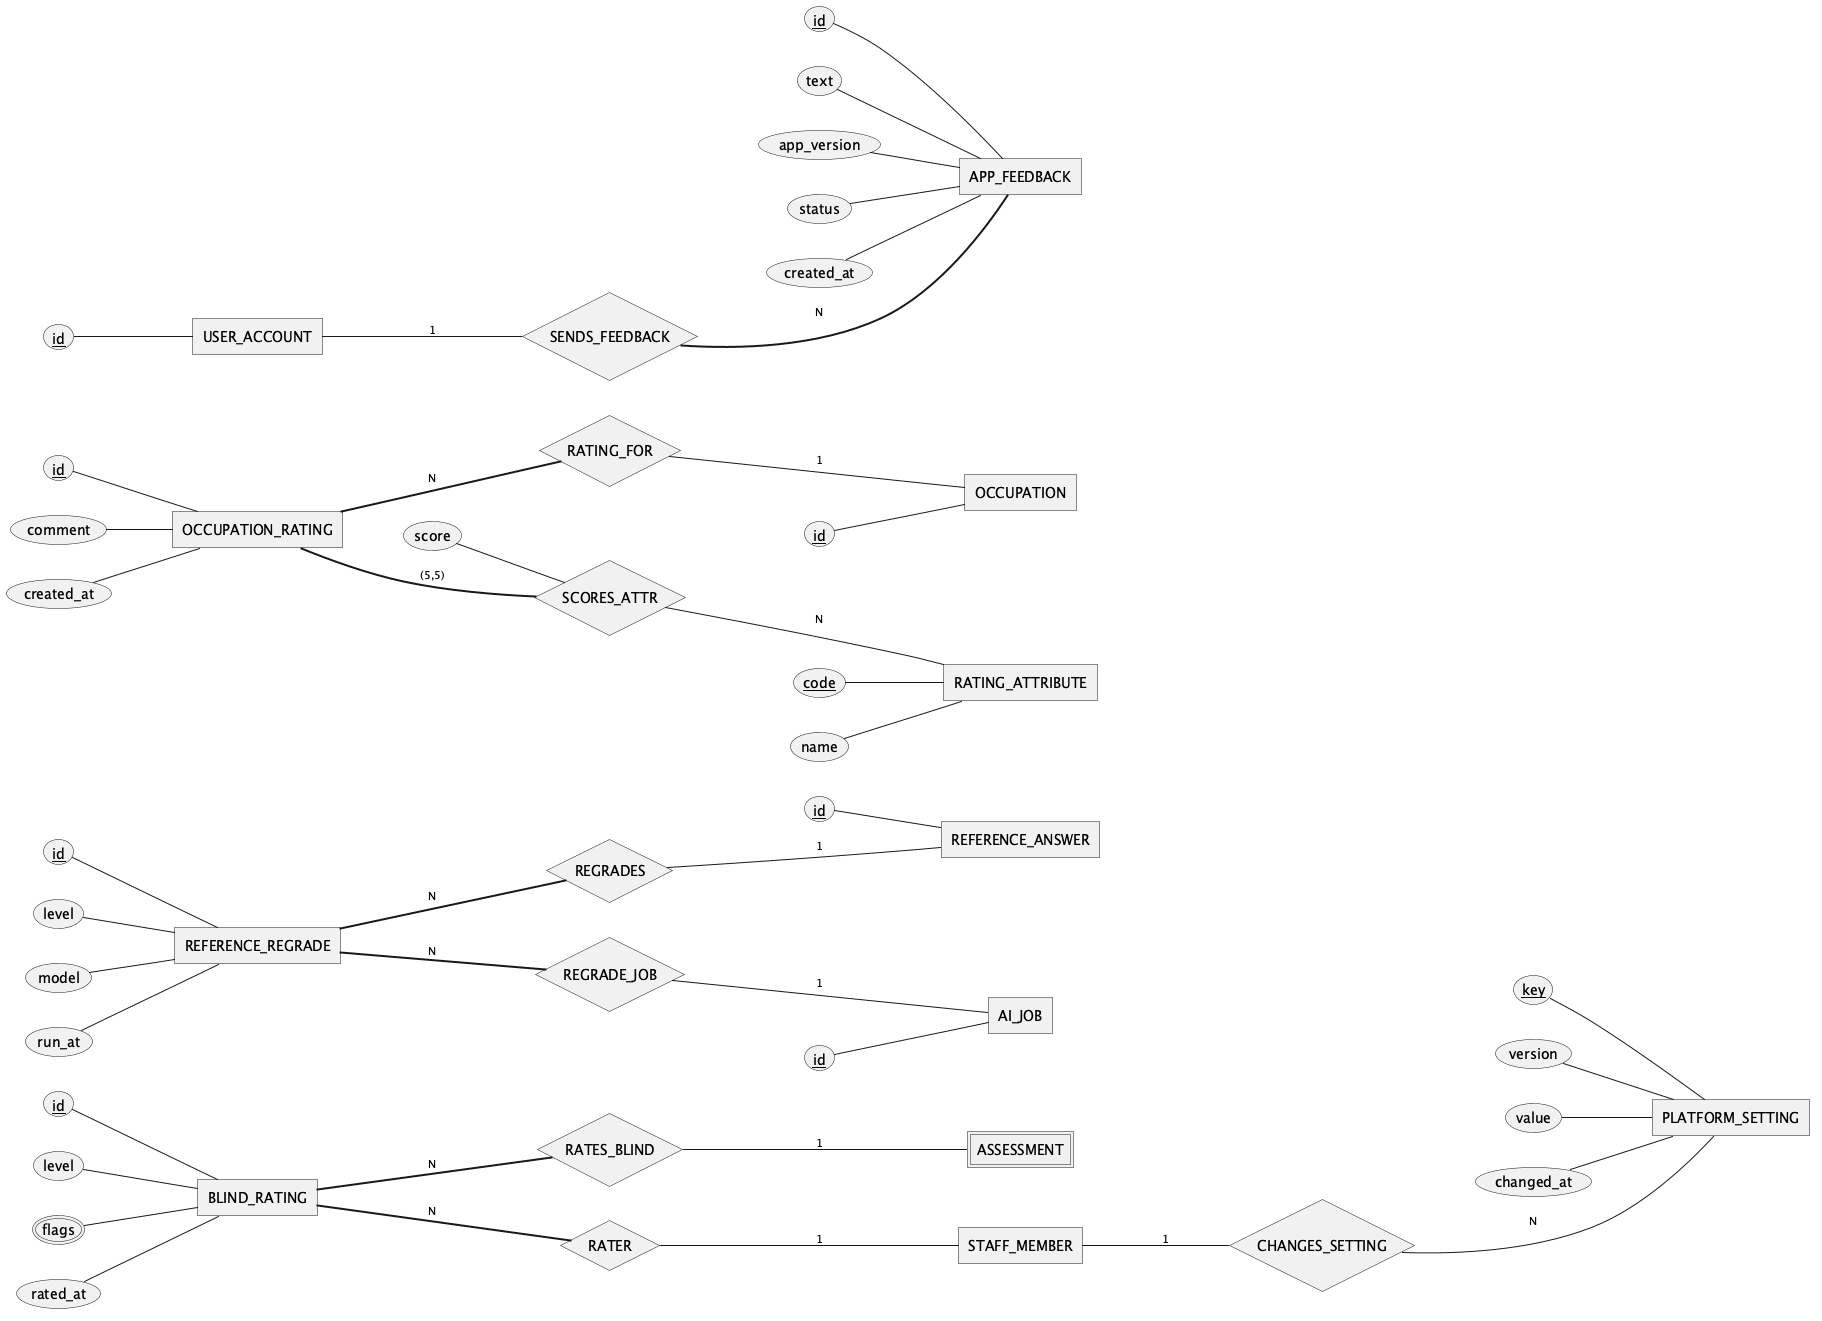
\includegraphics[width=\linewidth,height=0.86\textwidth,keepaspectratio,keepaspectratio]{figures/ERD-01b_QualityAndFeedback.png}
\caption{Entity--relationship diagram ERD-01b: Grading quality and feedback}
\end{figure}
\end{landscape}

\begin{landscape}
\begin{figure}[H]
\centering
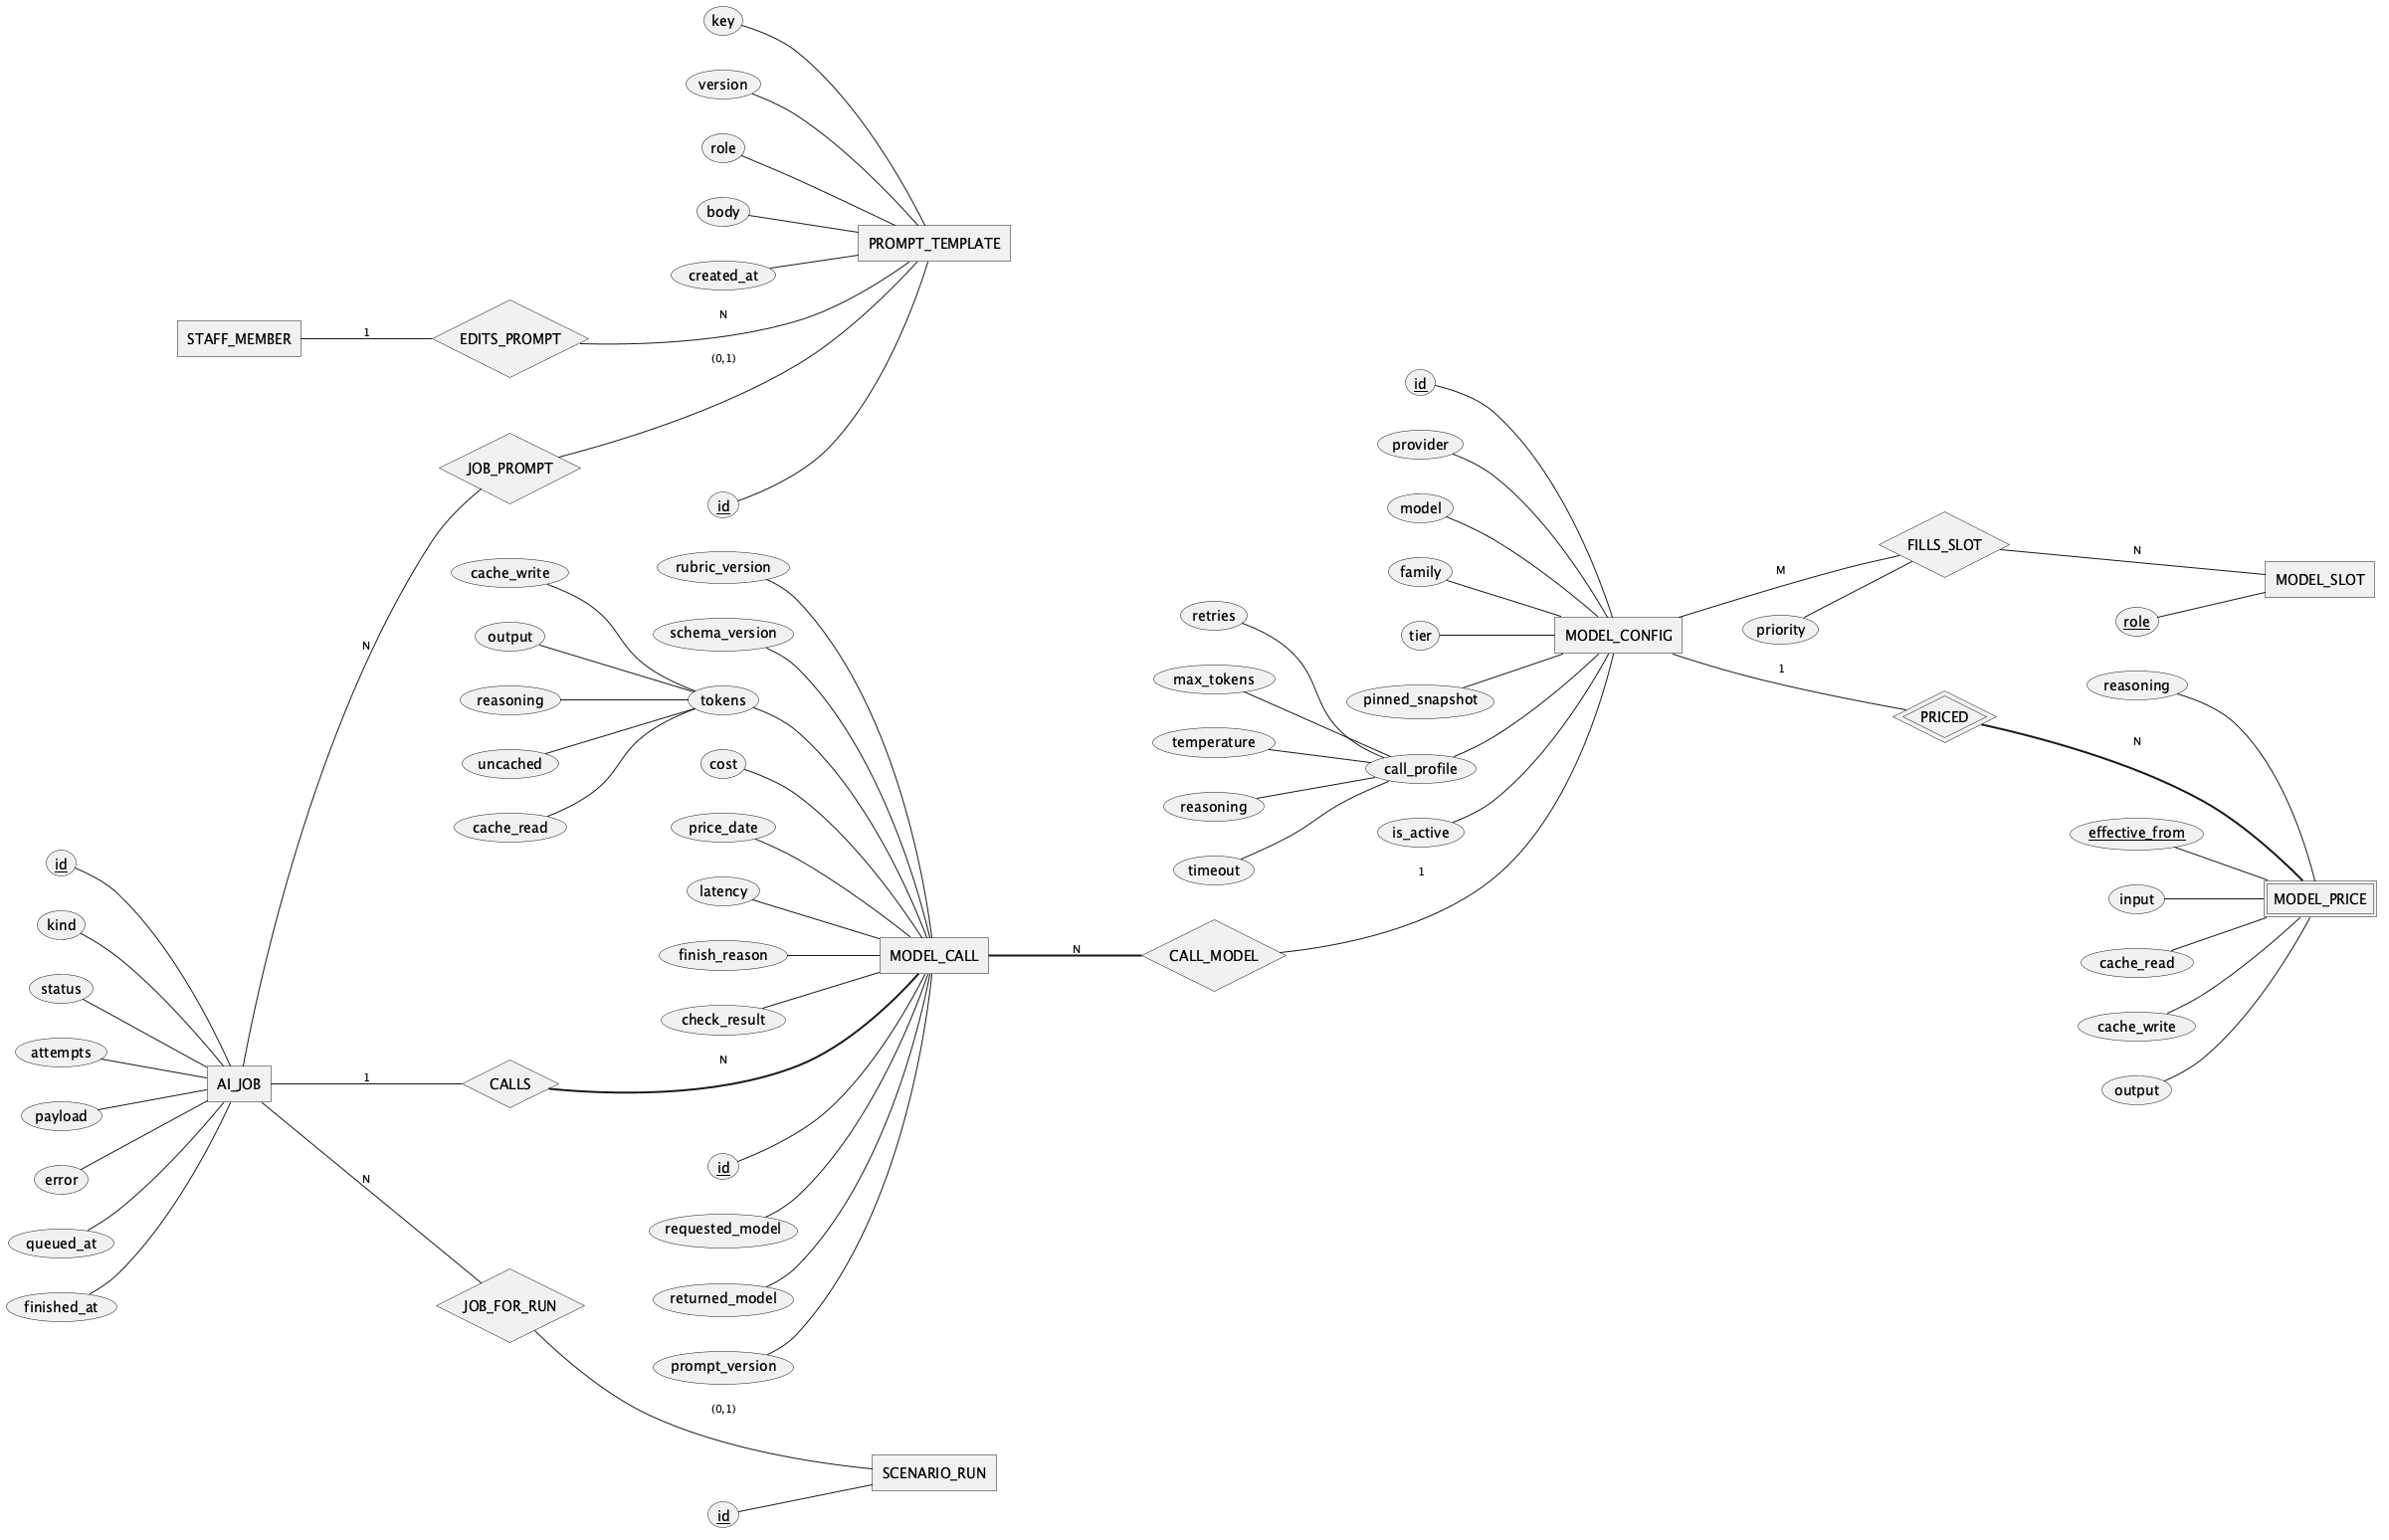
\includegraphics[width=\linewidth,height=0.86\textwidth,keepaspectratio,keepaspectratio]{figures/ERD-01c_AiOperations.png}
\caption{Entity--relationship diagram ERD-01c: AI operations}
\end{figure}
\end{landscape}

\begin{landscape}
\begin{figure}[H]
\centering
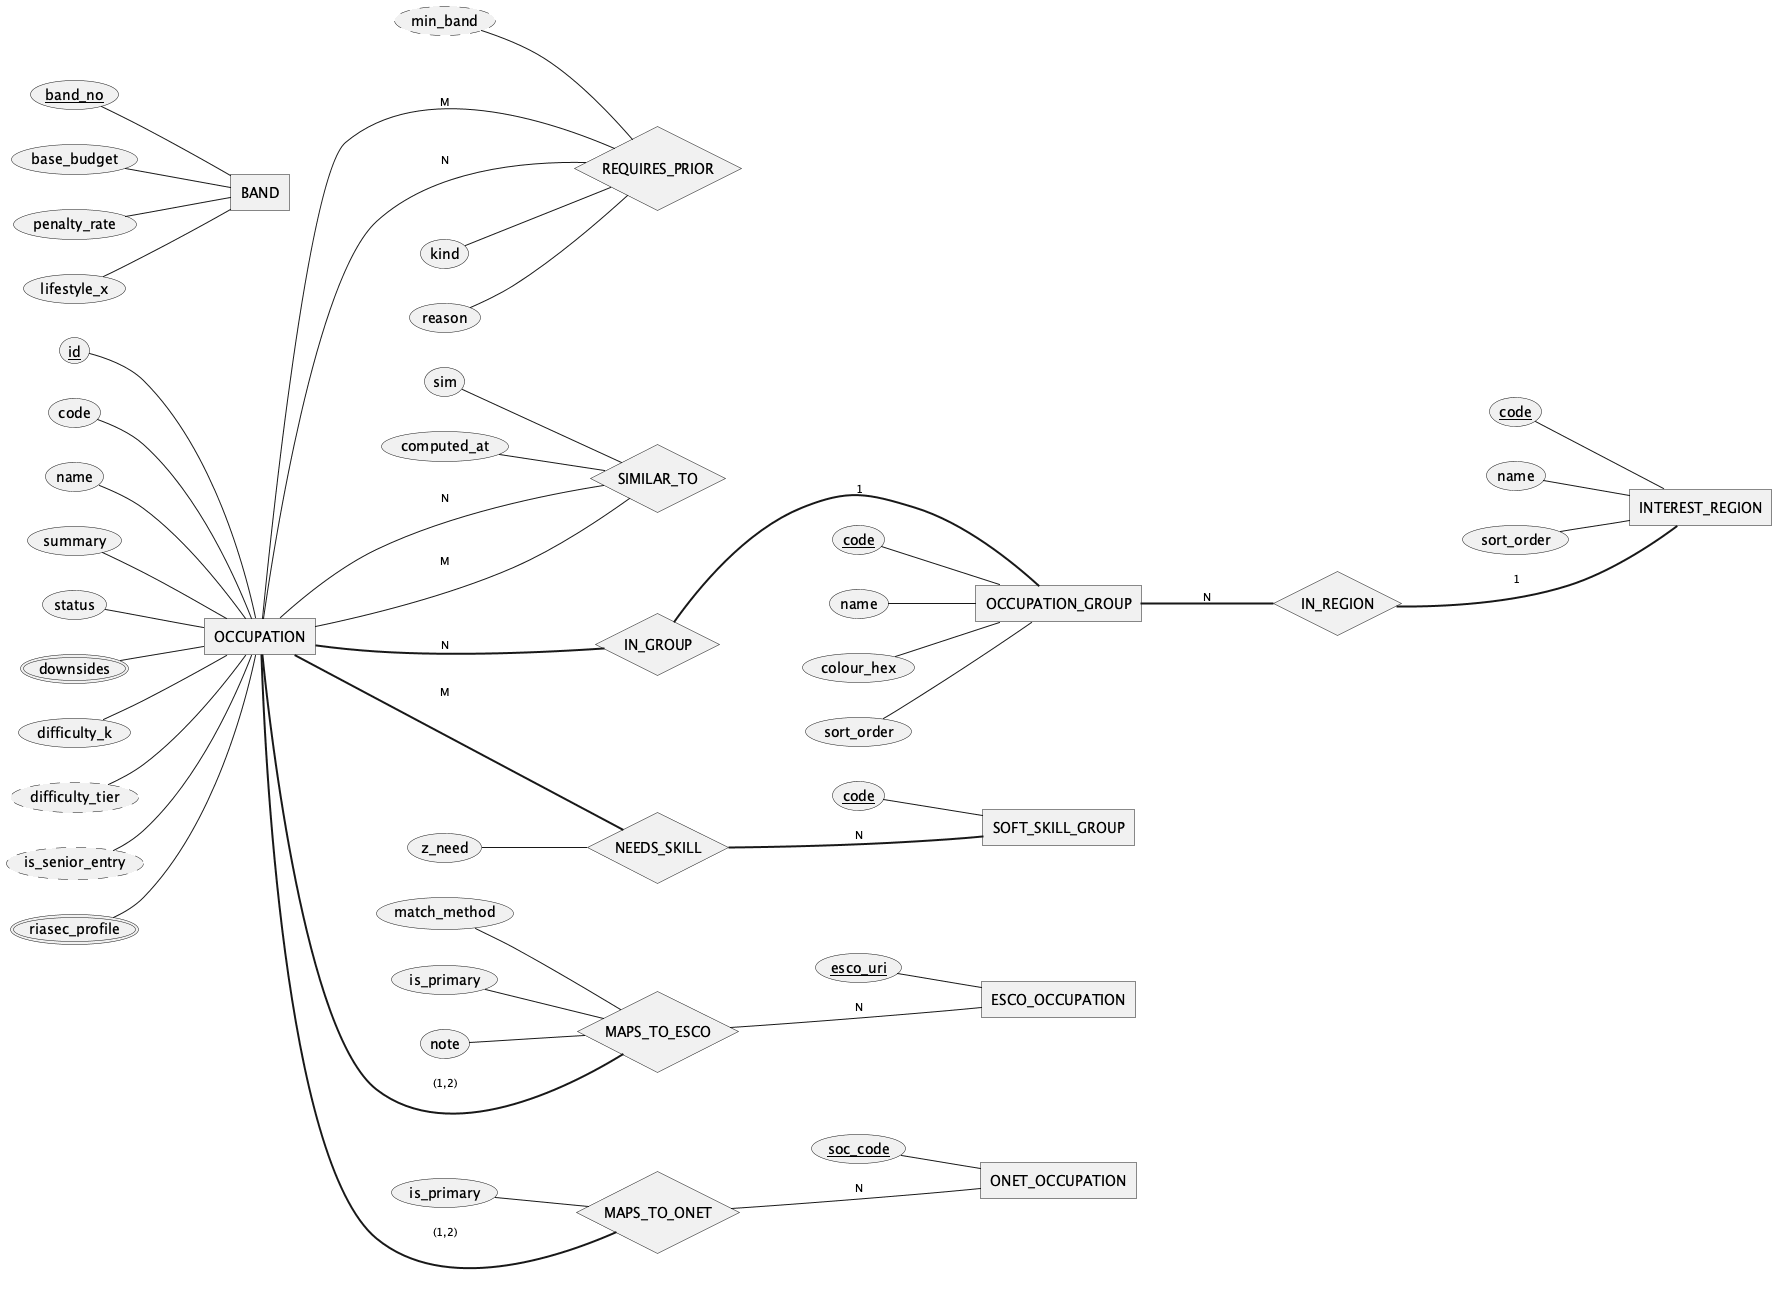
\includegraphics[width=\linewidth,height=0.86\textwidth,keepaspectratio,keepaspectratio]{figures/ERD-02a_Occupations.png}
\caption{Entity--relationship diagram ERD-02a: Occupations and interest regions}
\end{figure}
\end{landscape}

\begin{landscape}
\begin{figure}[H]
\centering
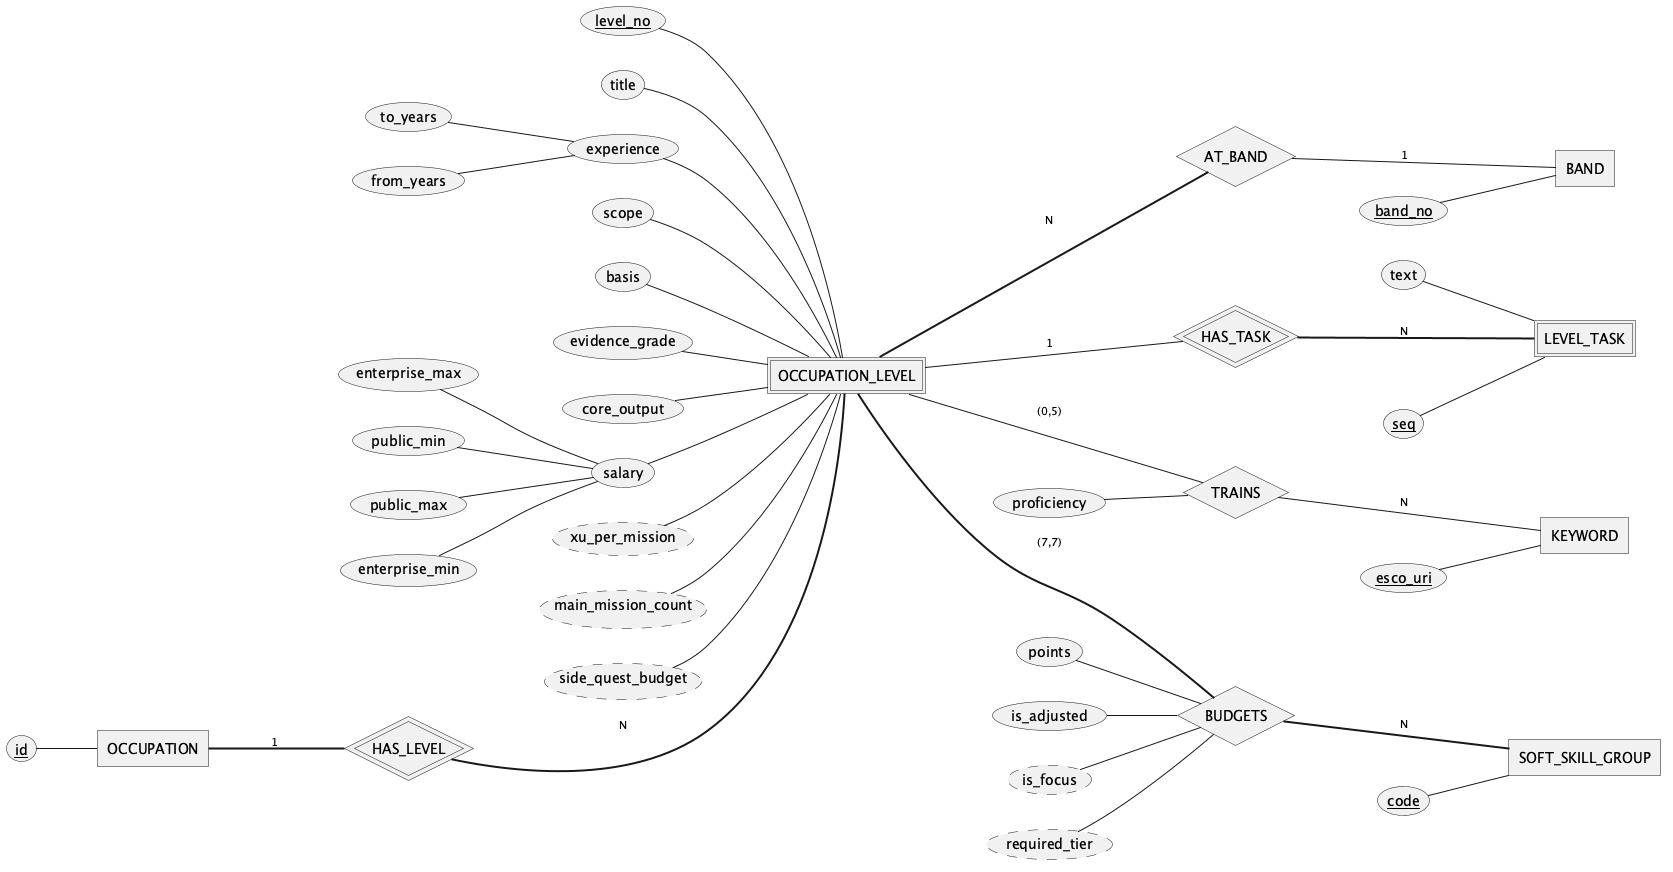
\includegraphics[width=\linewidth,height=0.86\textwidth,keepaspectratio,keepaspectratio]{figures/ERD-02b_LevelsAndTasks.png}
\caption{Entity--relationship diagram ERD-02b: Occupation levels and tasks}
\end{figure}
\end{landscape}

\begin{landscape}
\begin{figure}[H]
\centering
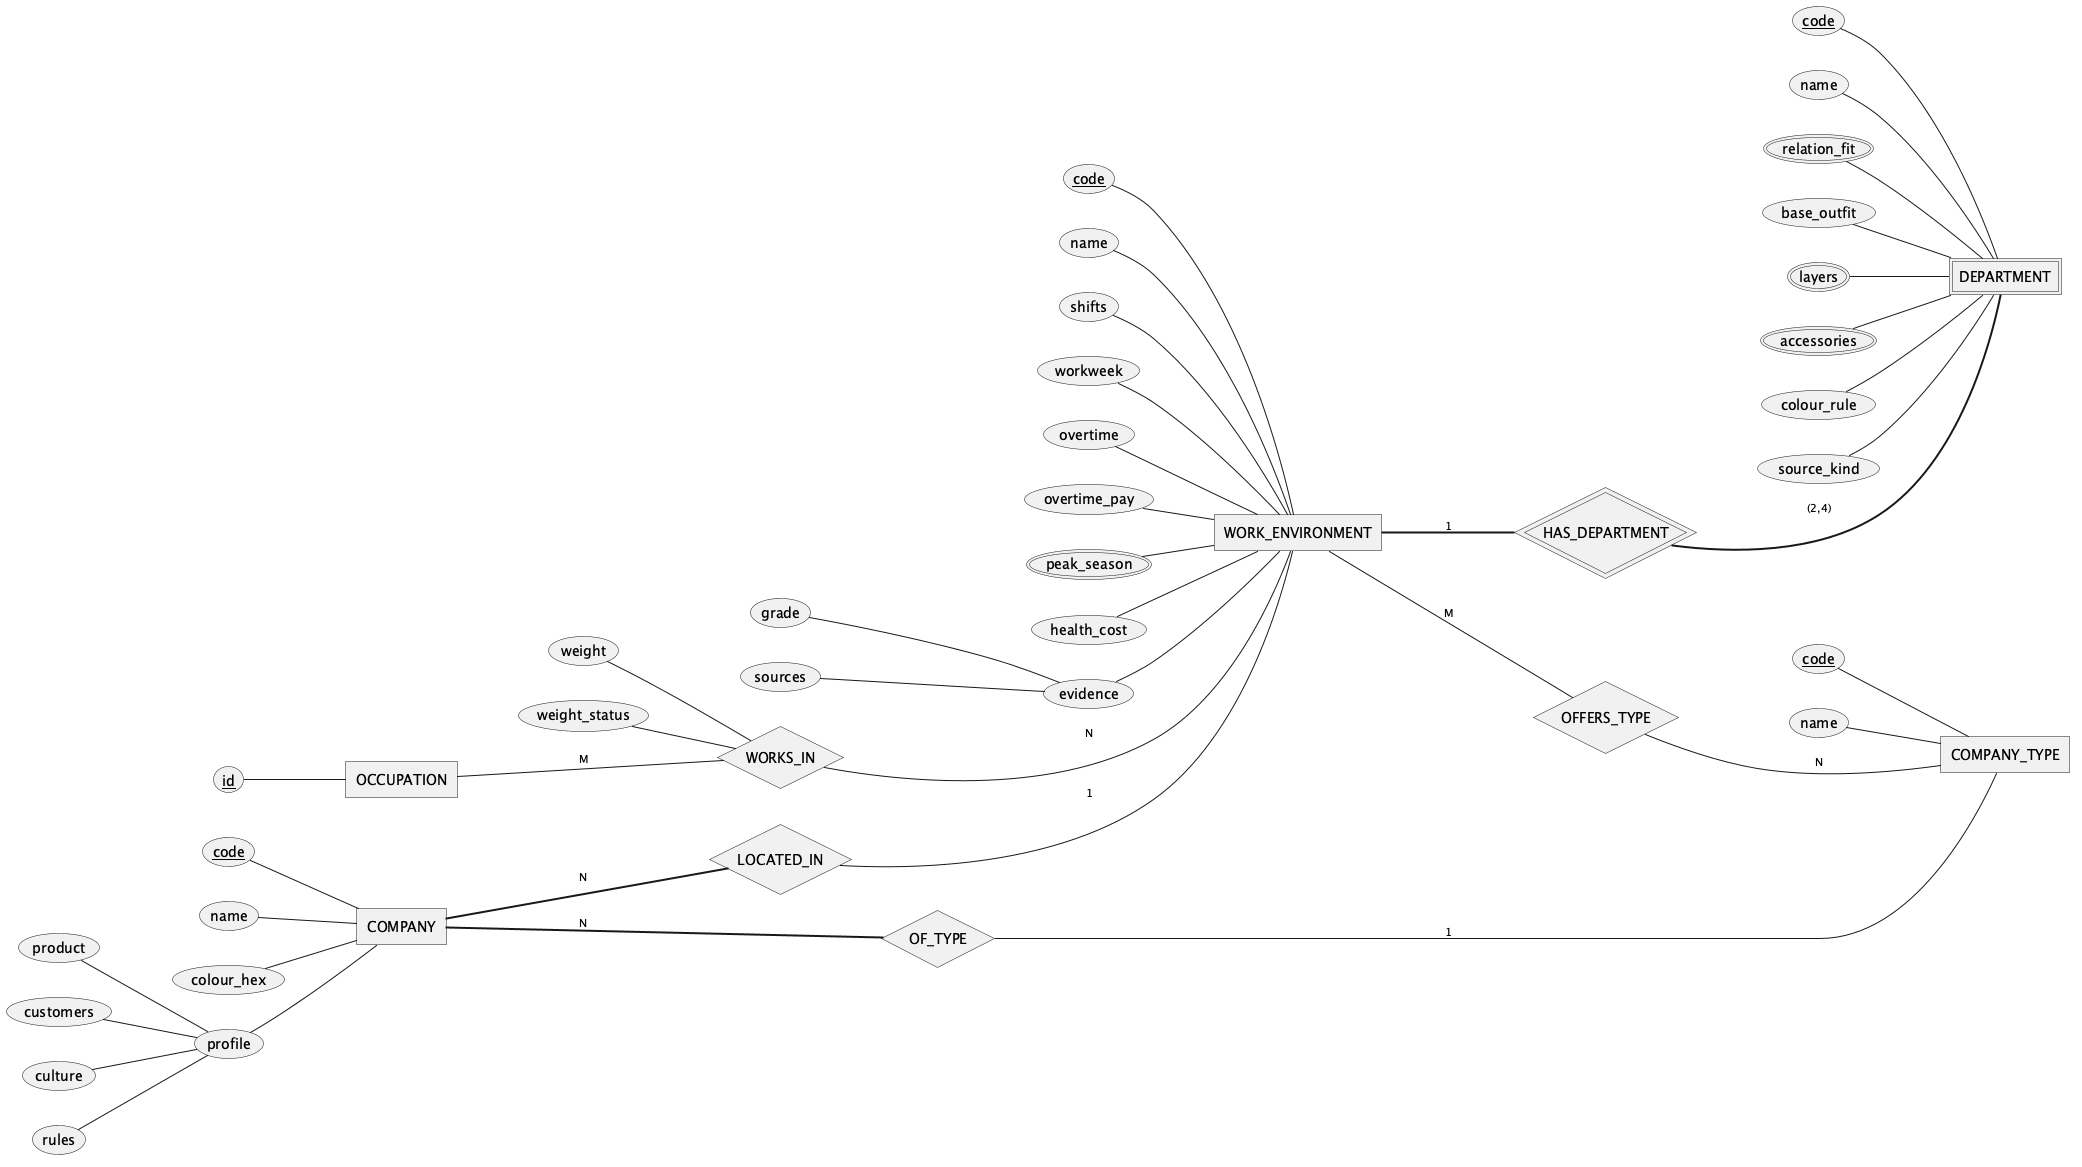
\includegraphics[width=\linewidth,height=0.86\textwidth,keepaspectratio,keepaspectratio]{figures/ERD-02c_WorkEnvironments.png}
\caption{Entity--relationship diagram ERD-02c: Work environments}
\end{figure}
\end{landscape}

\begin{landscape}
\begin{figure}[H]
\centering
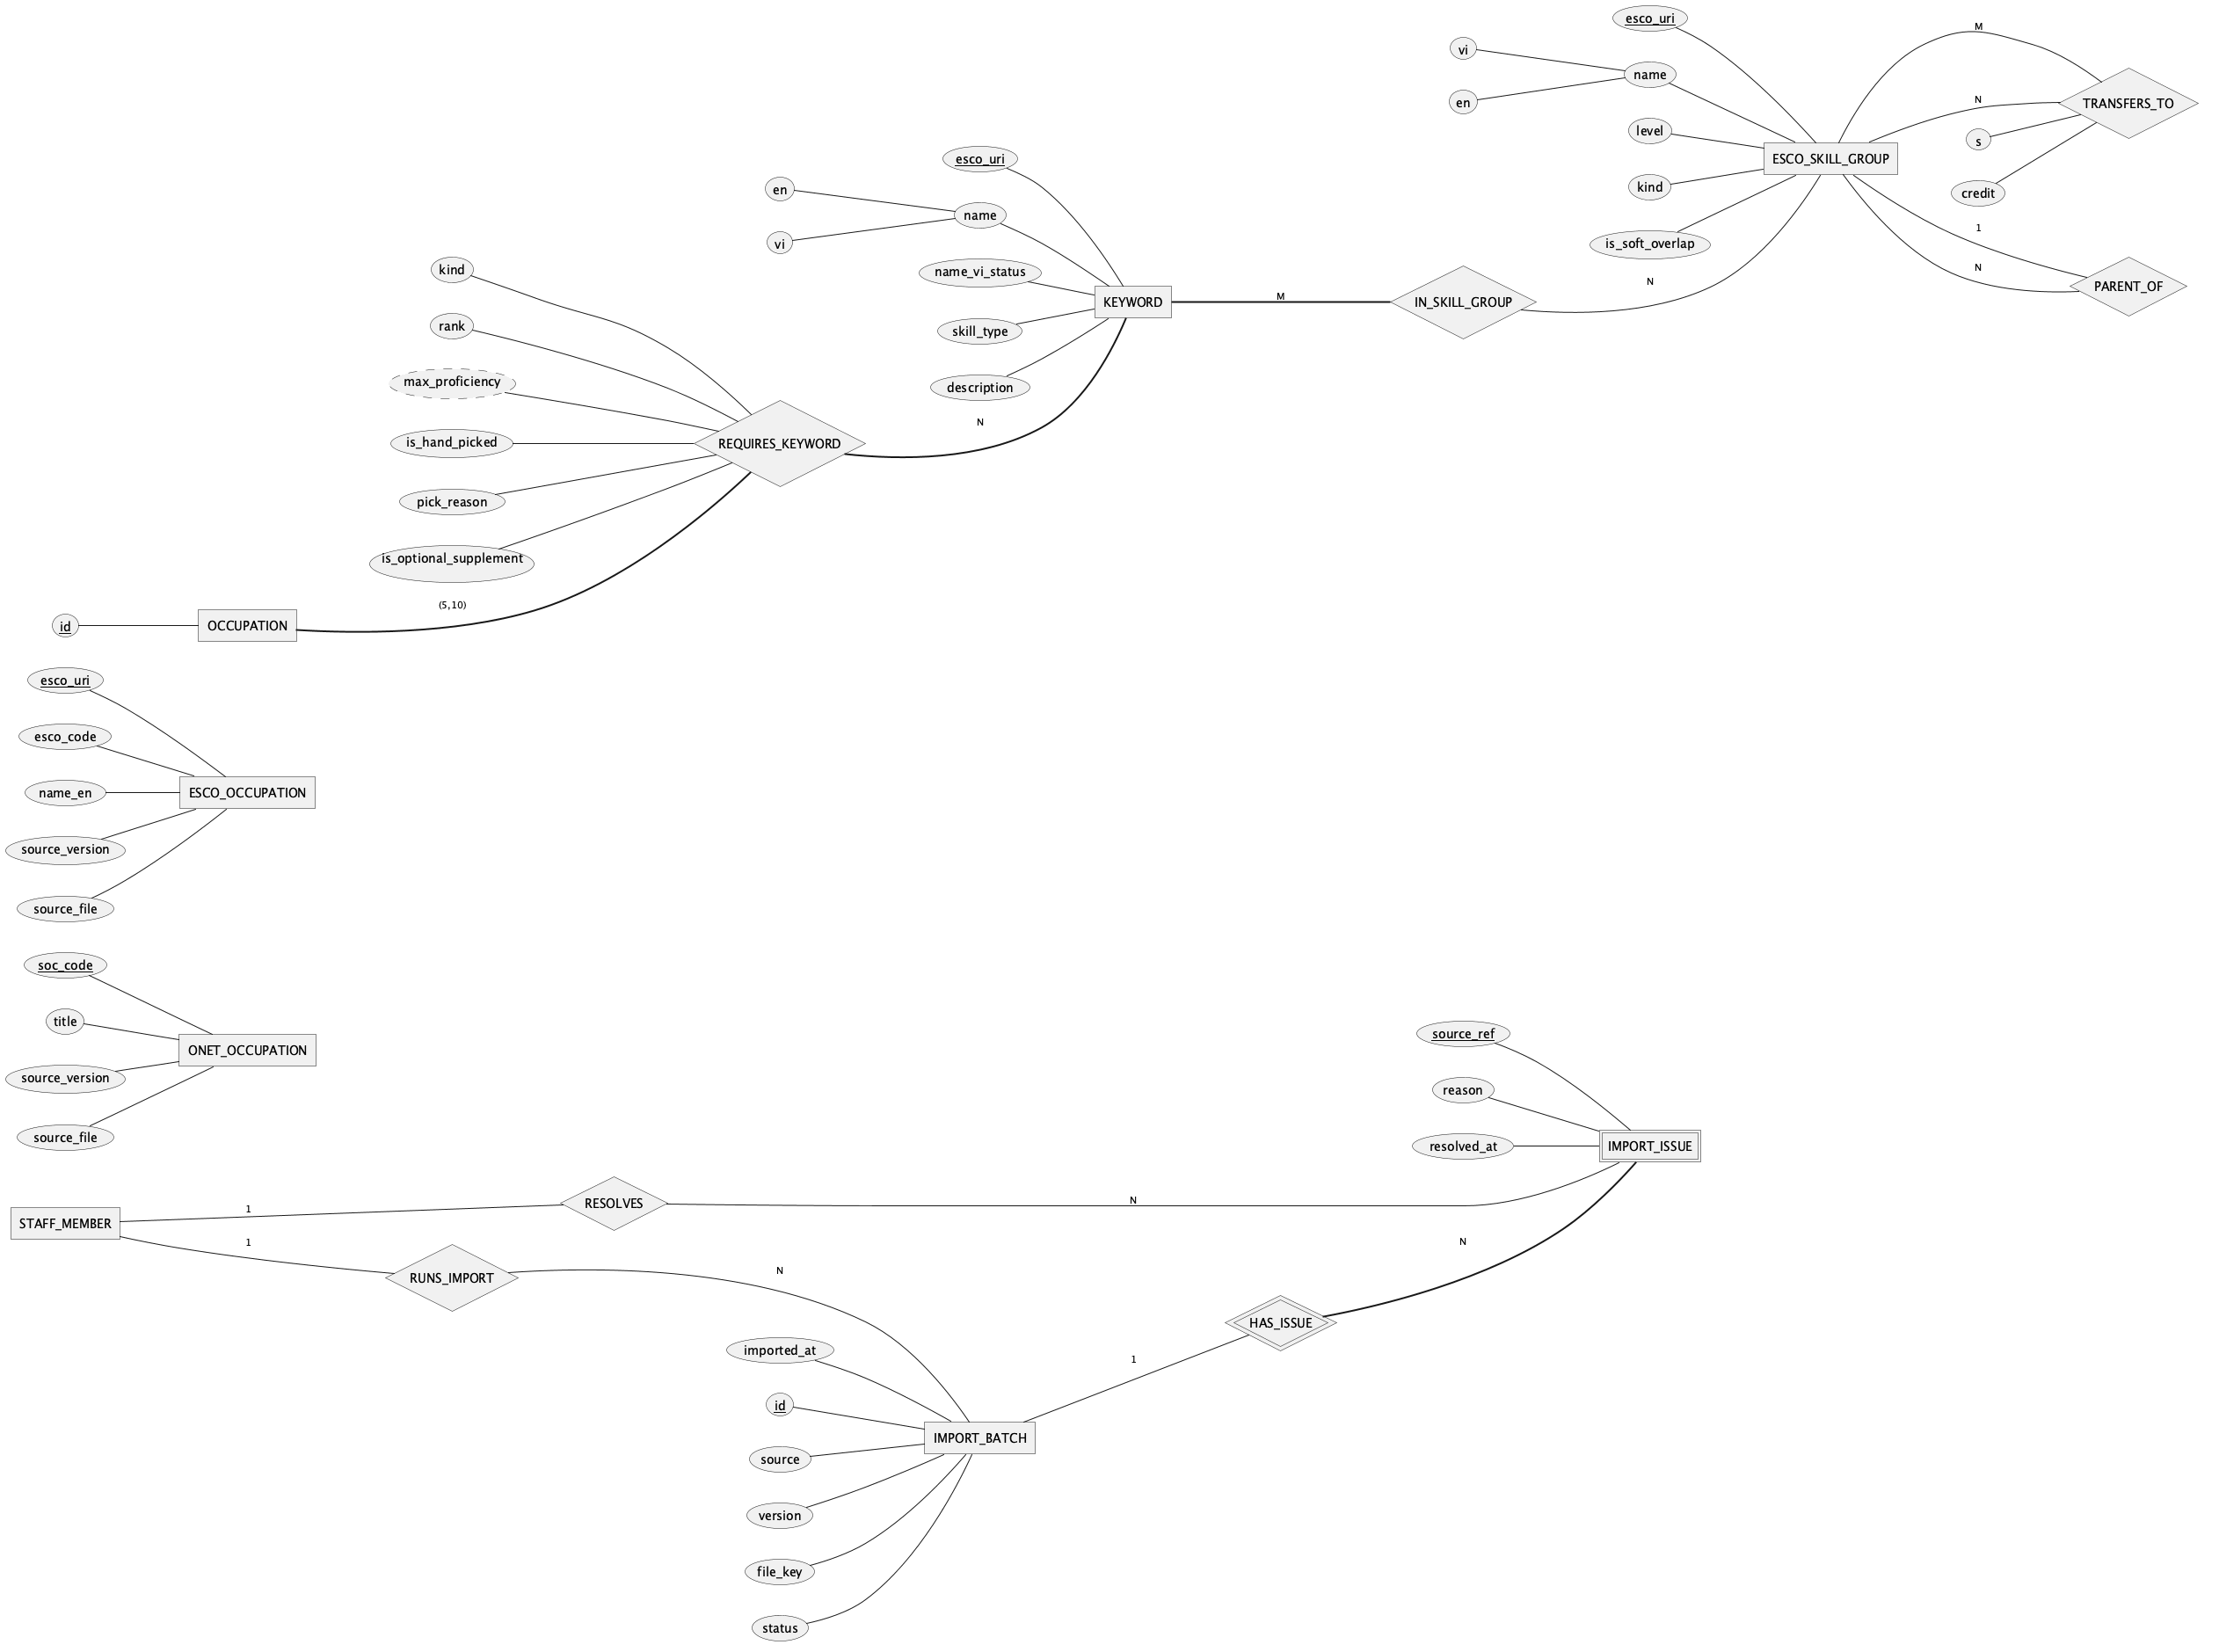
\includegraphics[width=\linewidth,height=0.86\textwidth,keepaspectratio,keepaspectratio]{figures/ERD-02d_ReferenceAndKeywords.png}
\caption{Entity--relationship diagram ERD-02d: Reference data and keywords}
\end{figure}
\end{landscape}

\begin{landscape}
\begin{figure}[H]
\centering
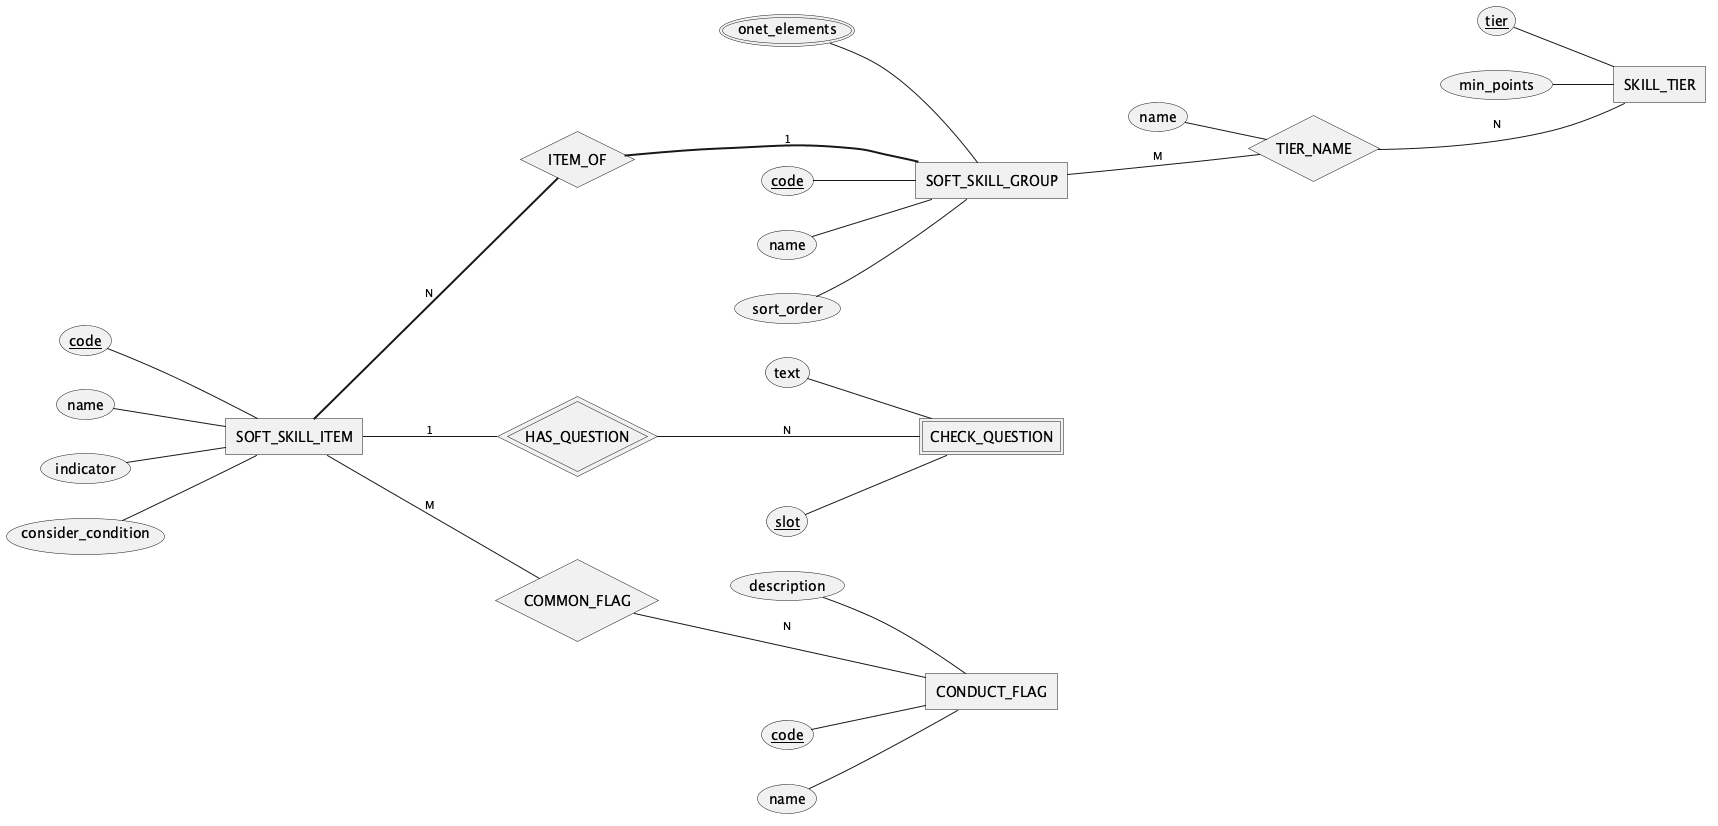
\includegraphics[width=\linewidth,height=0.86\textwidth,keepaspectratio,keepaspectratio]{figures/ERD-02e_SoftSkills.png}
\caption{Entity--relationship diagram ERD-02e: Soft skills}
\end{figure}
\end{landscape}

\begin{figure}[H]
\centering
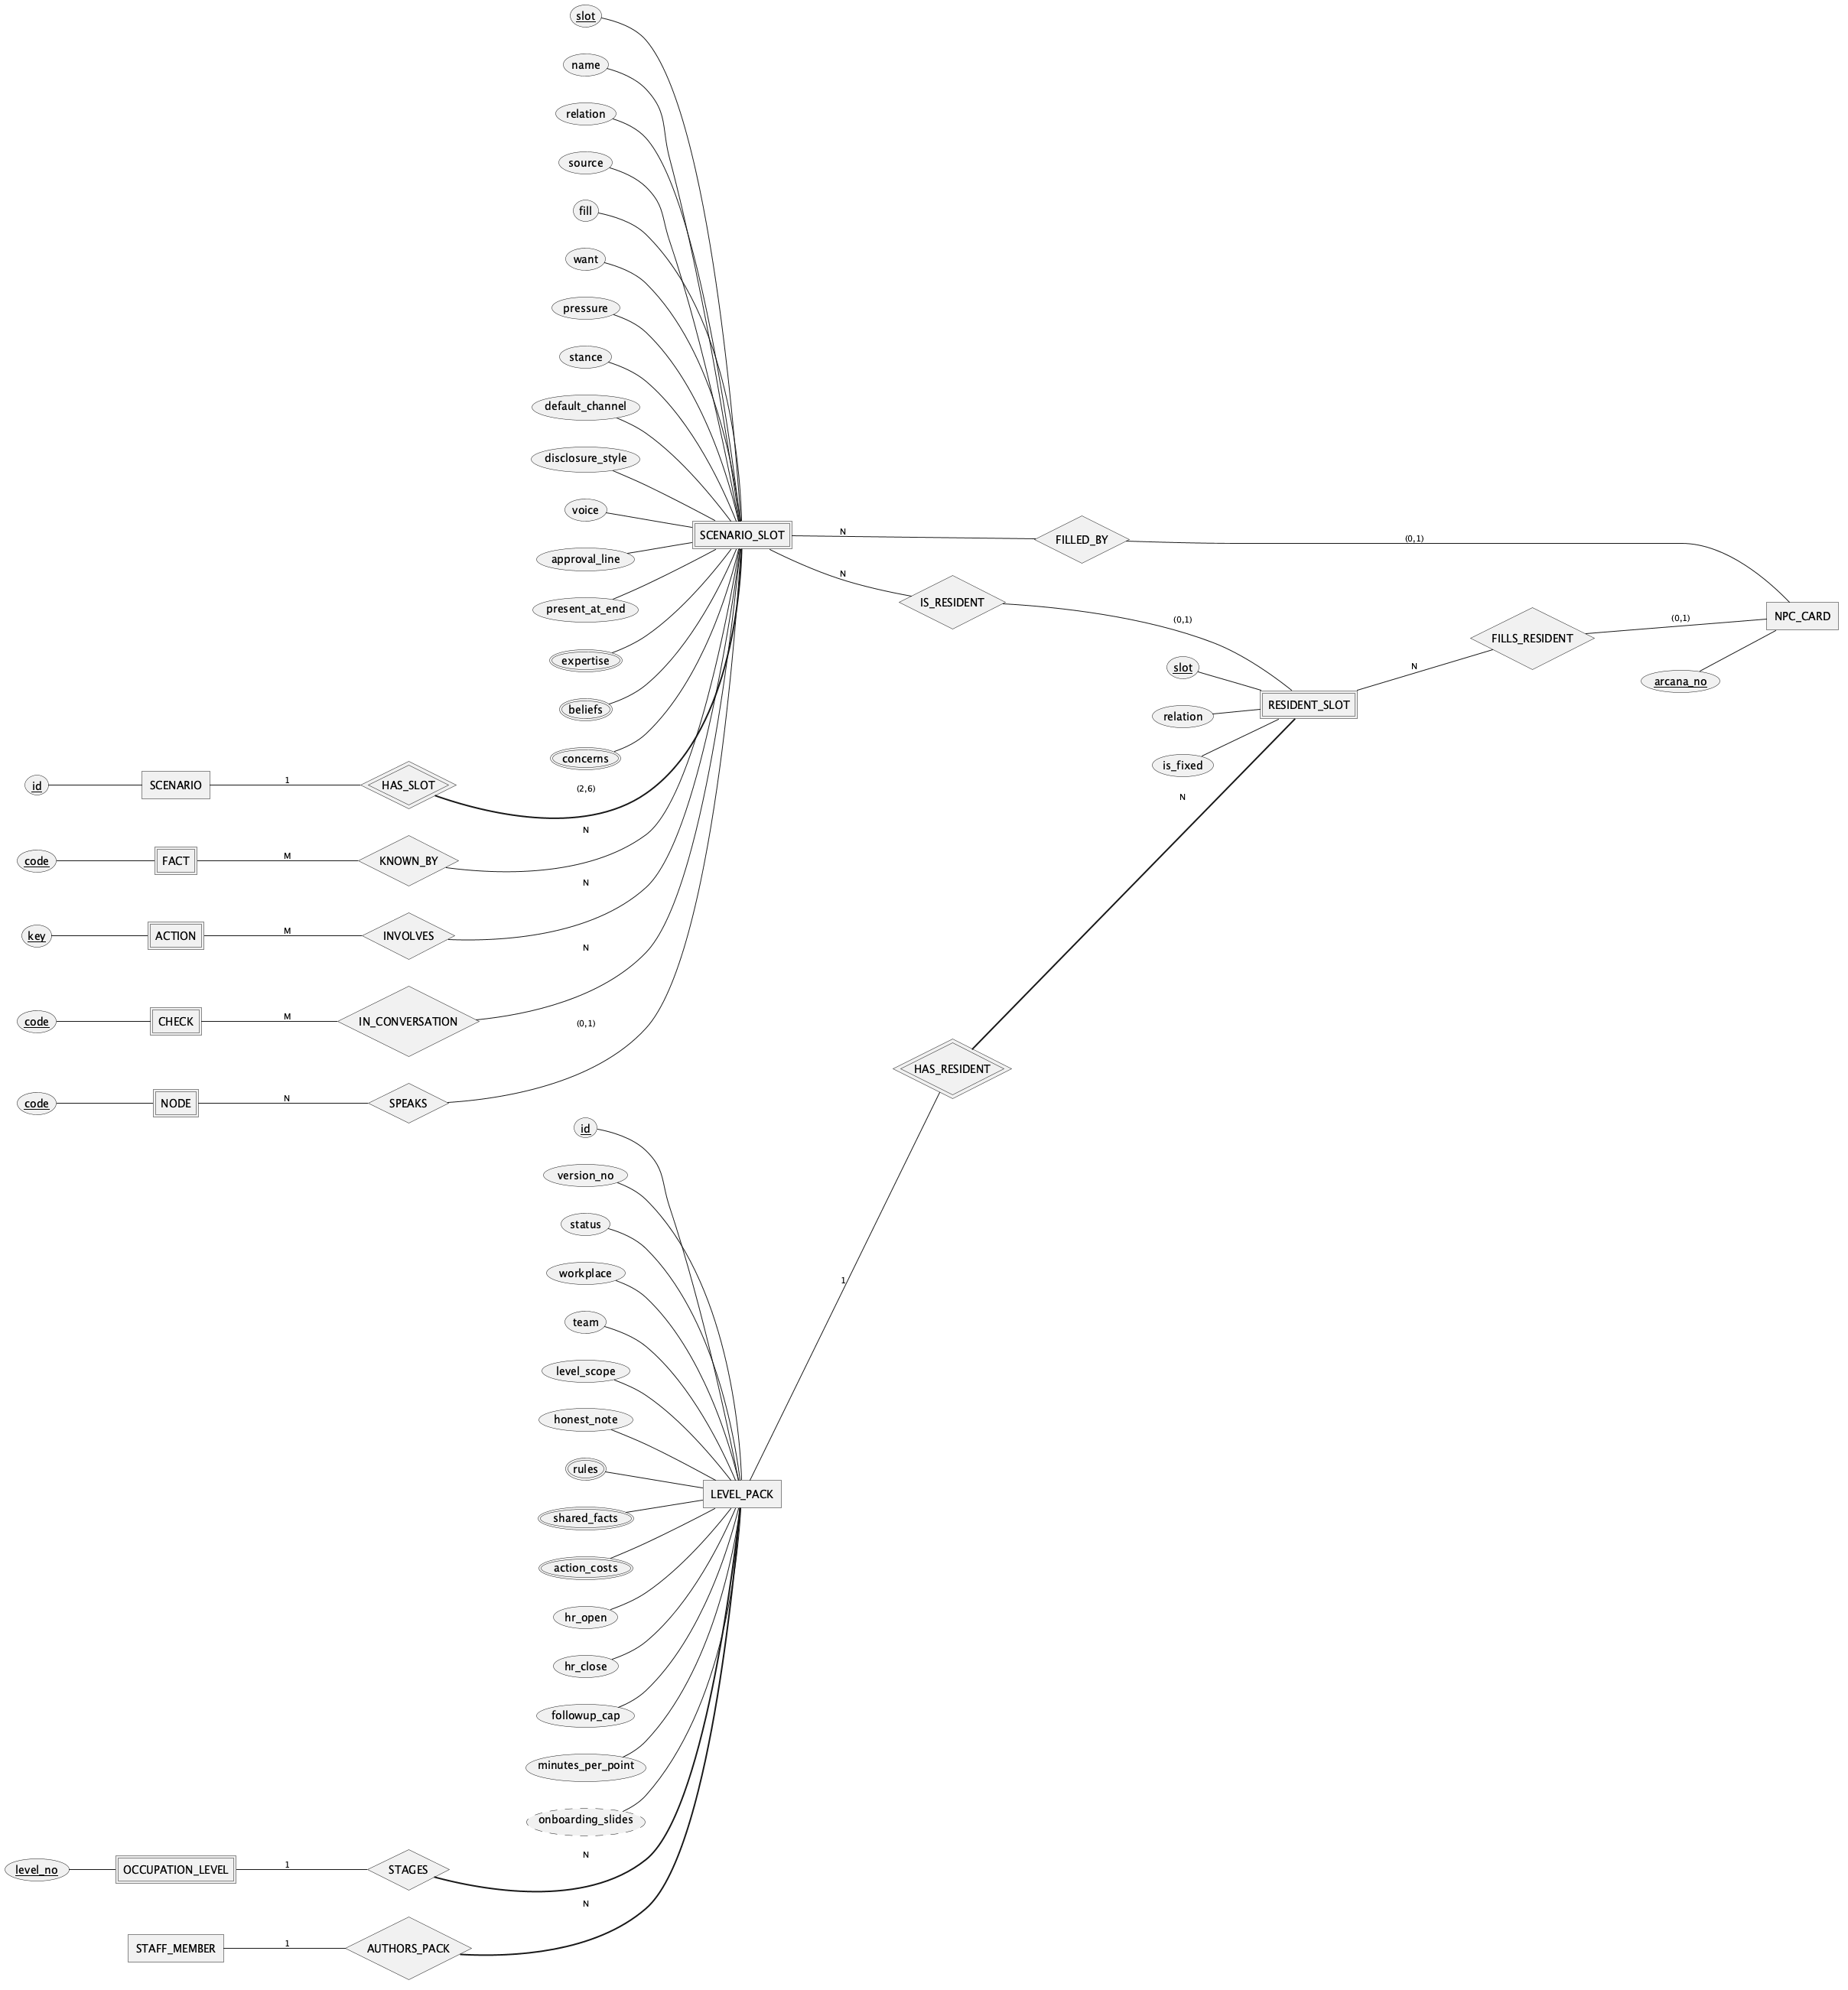
\includegraphics[width=\textwidth,height=0.9\textheight,keepaspectratio]{figures/ERD-03b_PackAndSlots.png}
\caption{Entity--relationship diagram ERD-03b: Level pack and scenario slots}
\end{figure}

\begin{figure}[H]
\centering
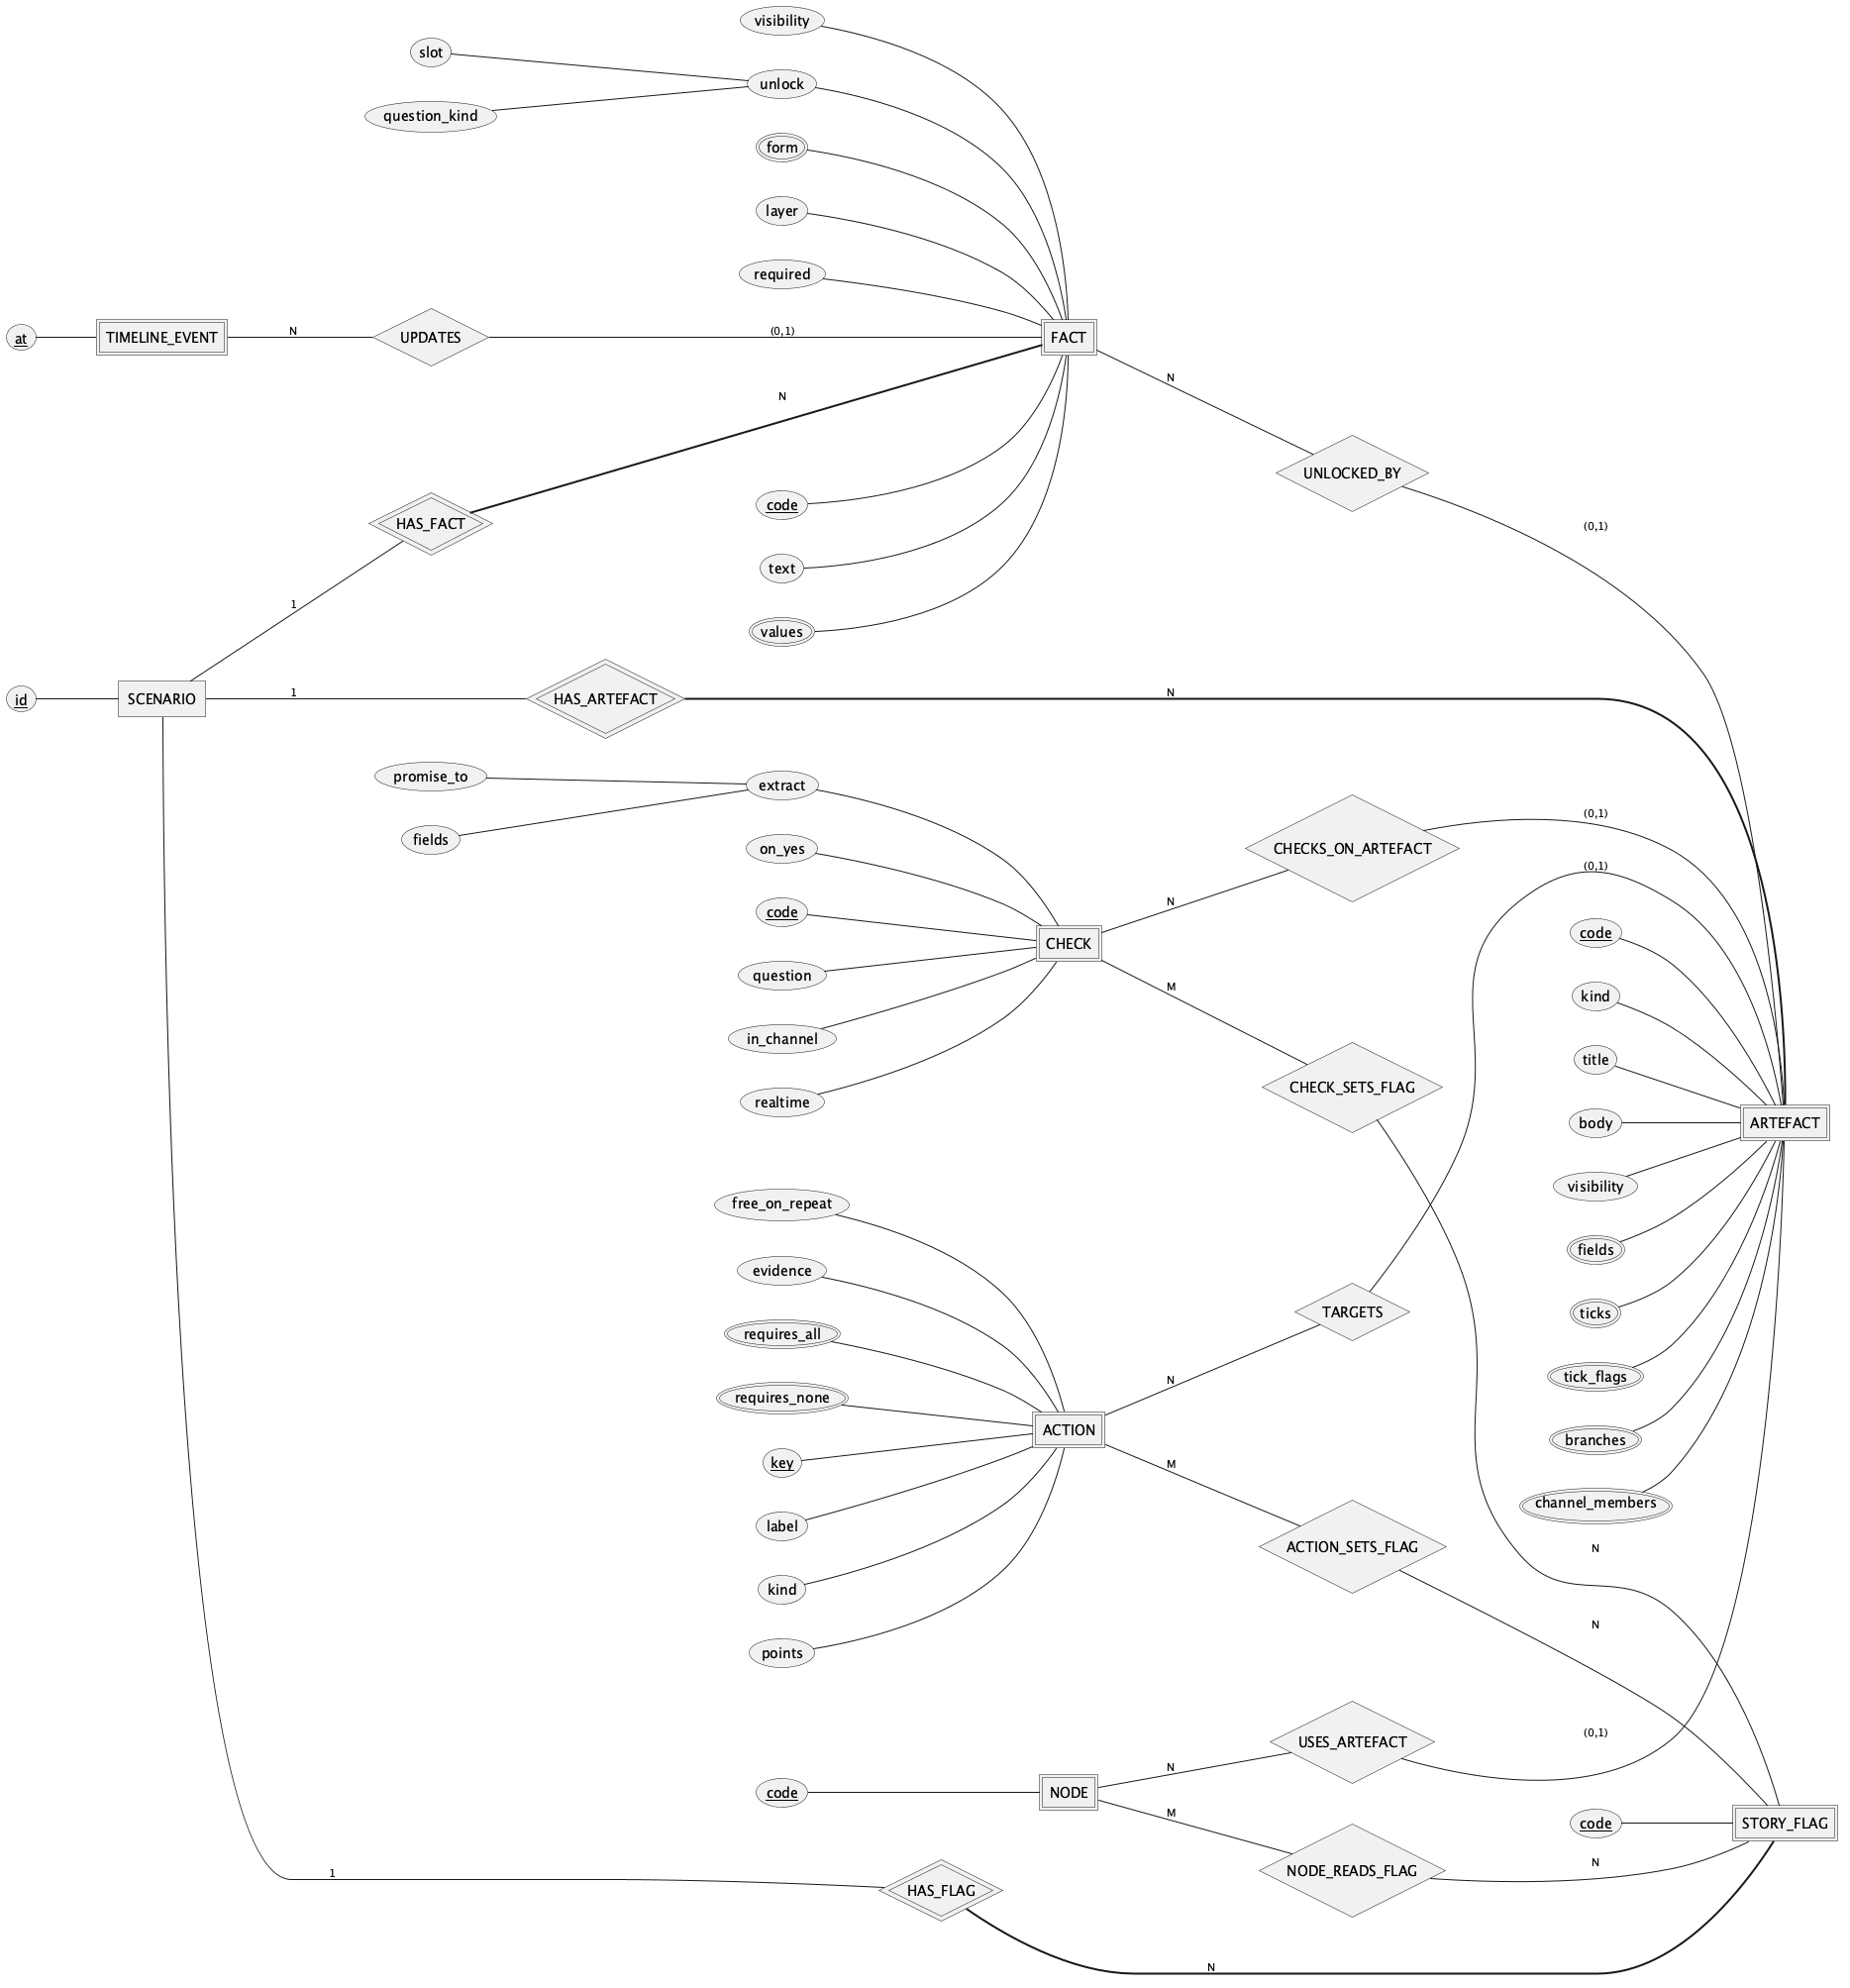
\includegraphics[width=\textwidth,height=0.9\textheight,keepaspectratio]{figures/ERD-03c_FactsAndActions.png}
\caption{Entity--relationship diagram ERD-03c: Scenario facts and actions}
\end{figure}

\begin{landscape}
\begin{figure}[H]
\centering
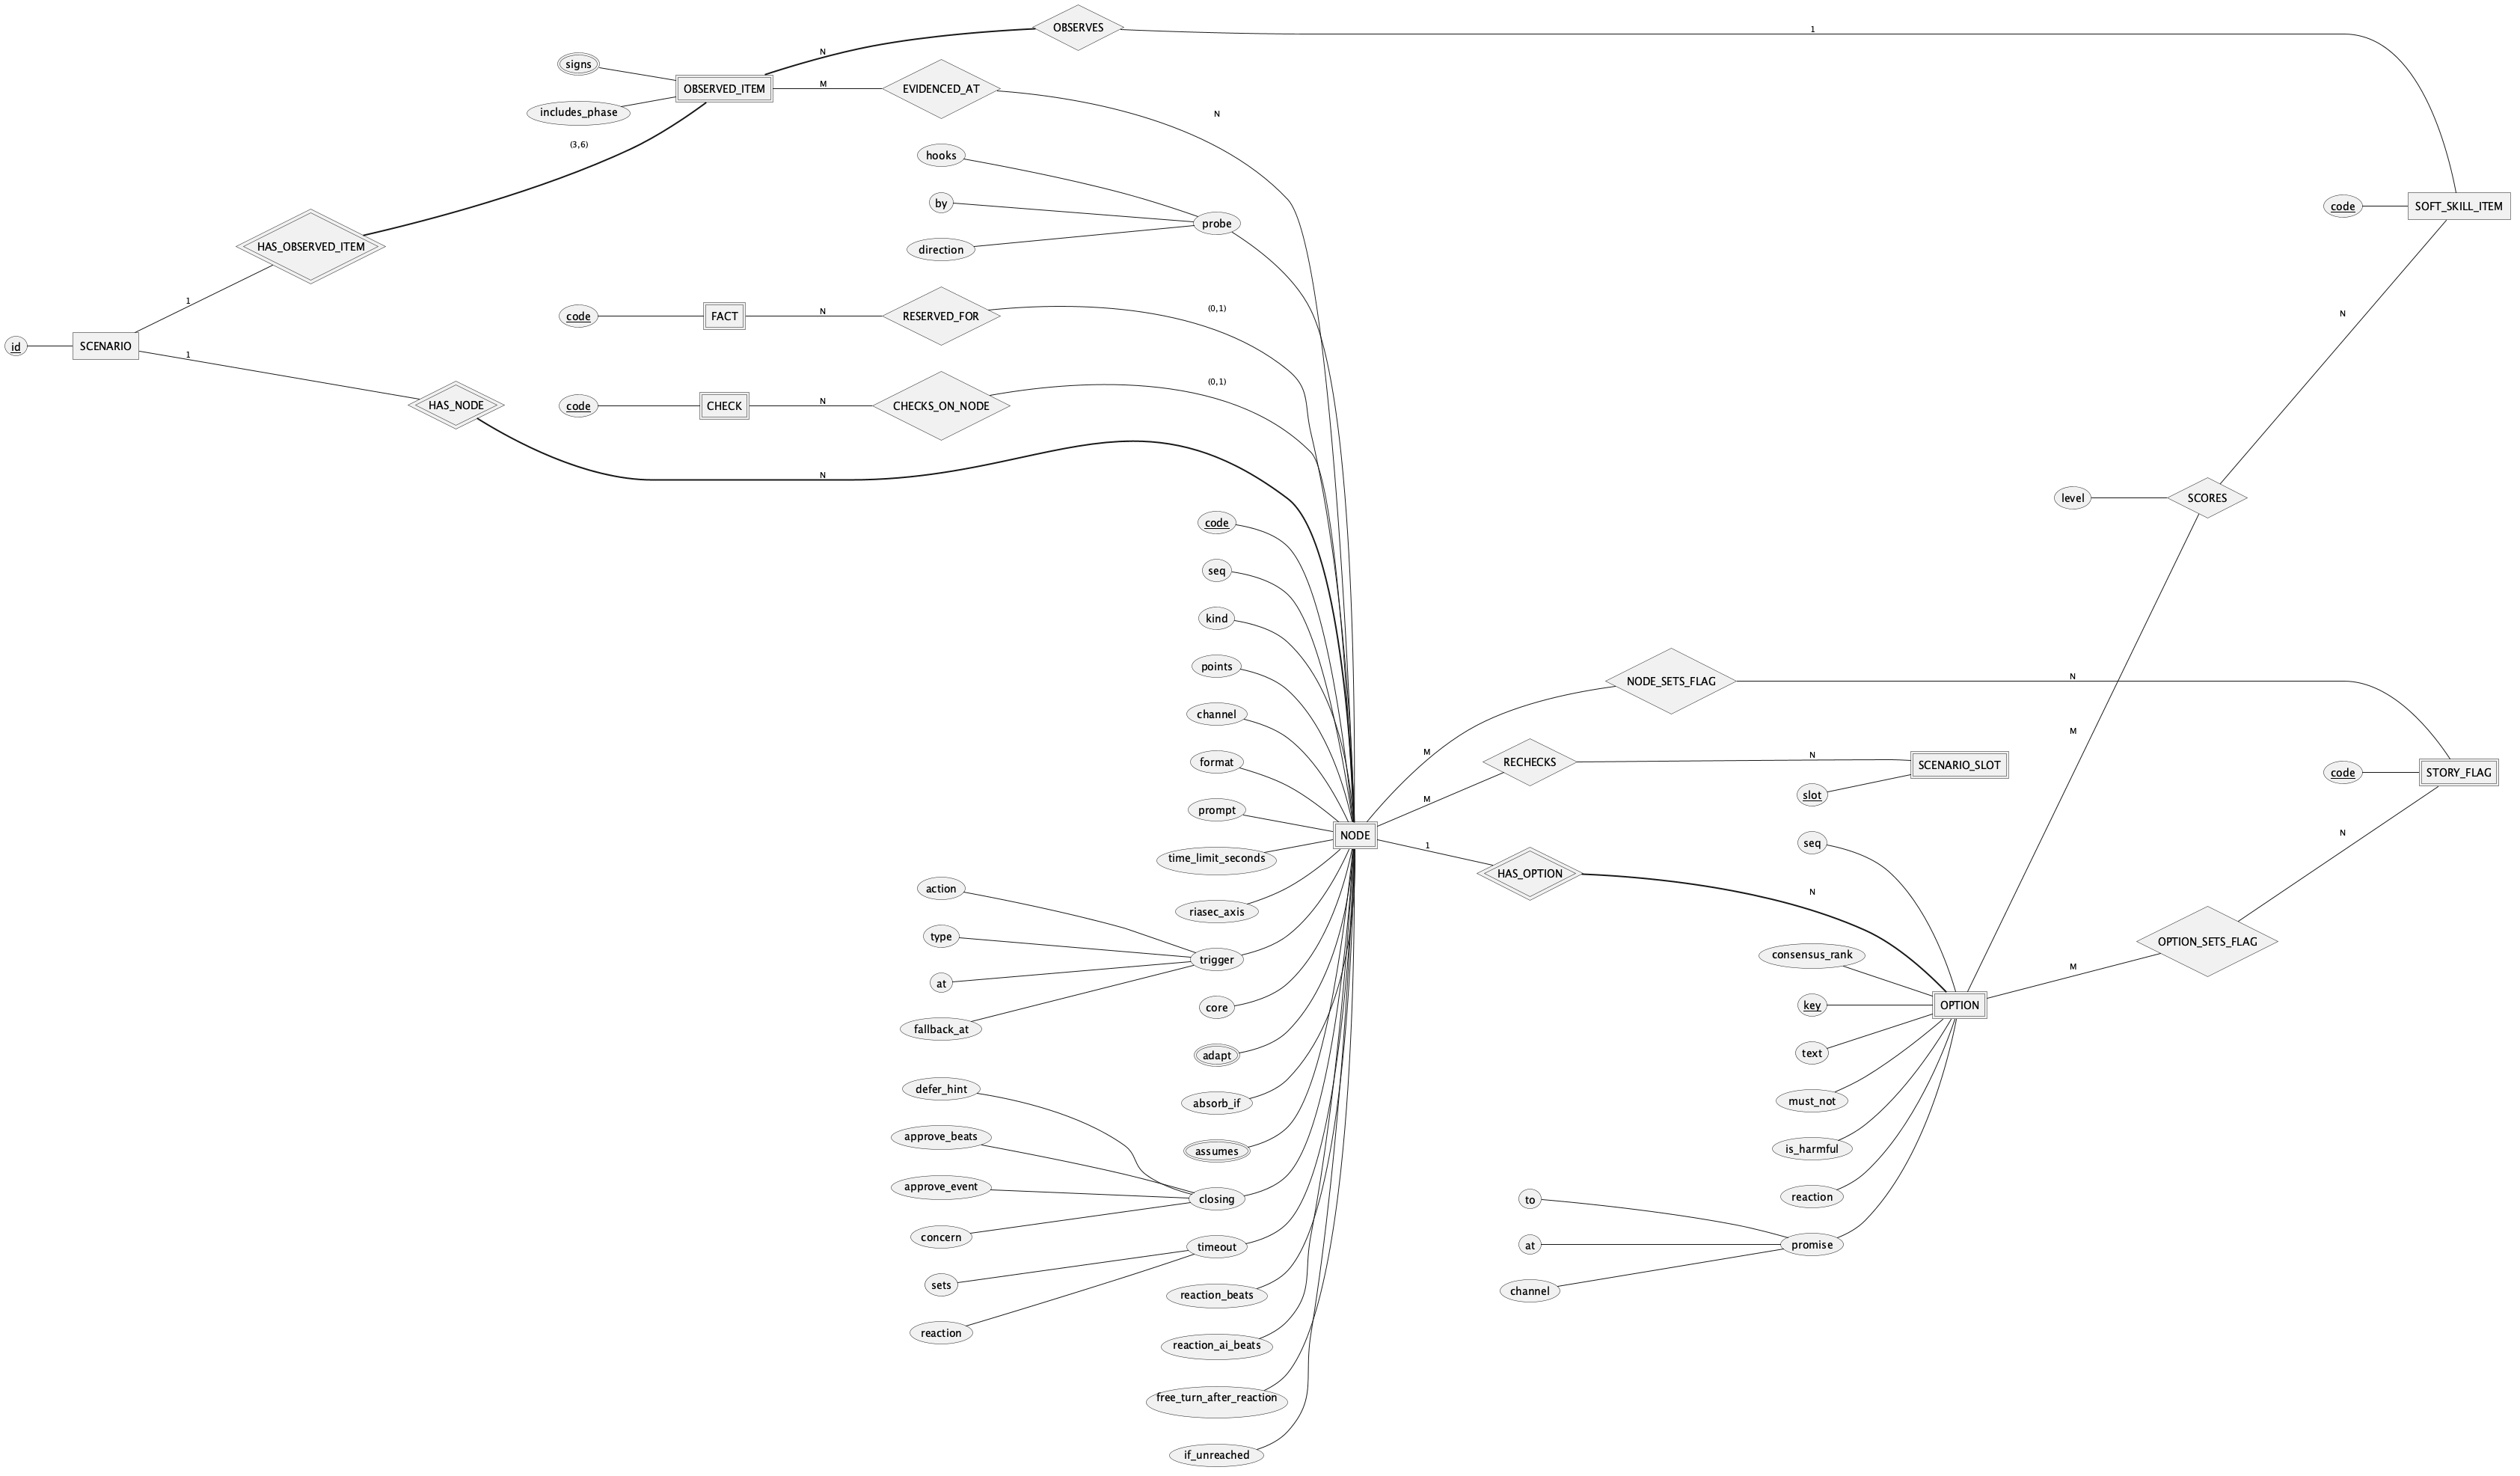
\includegraphics[width=\linewidth,height=0.86\textwidth,keepaspectratio,keepaspectratio]{figures/ERD-03d_Nodes.png}
\caption{Entity--relationship diagram ERD-03d: Scenario nodes and options}
\end{figure}
\end{landscape}

\begin{landscape}
\begin{figure}[H]
\centering
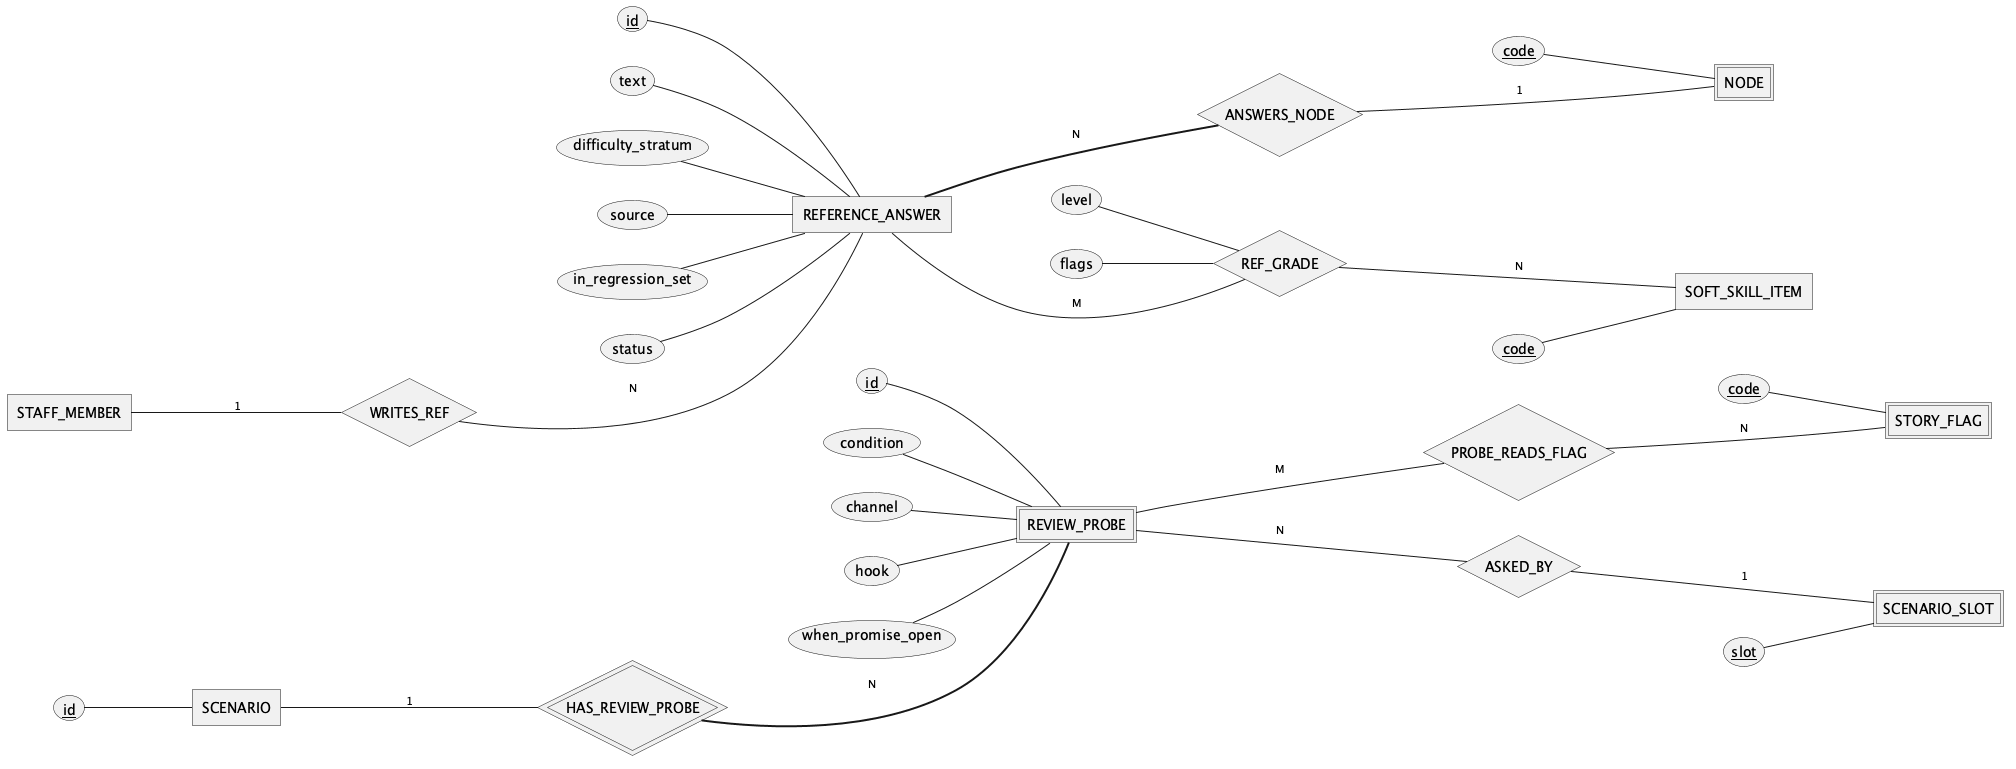
\includegraphics[width=\linewidth,height=0.86\textwidth,keepaspectratio,keepaspectratio]{figures/ERD-03e_ProbesAndAnswers.png}
\caption{Entity--relationship diagram ERD-03e: Review probes and reference answers}
\end{figure}
\end{landscape}

\begin{landscape}
\begin{figure}[H]
\centering
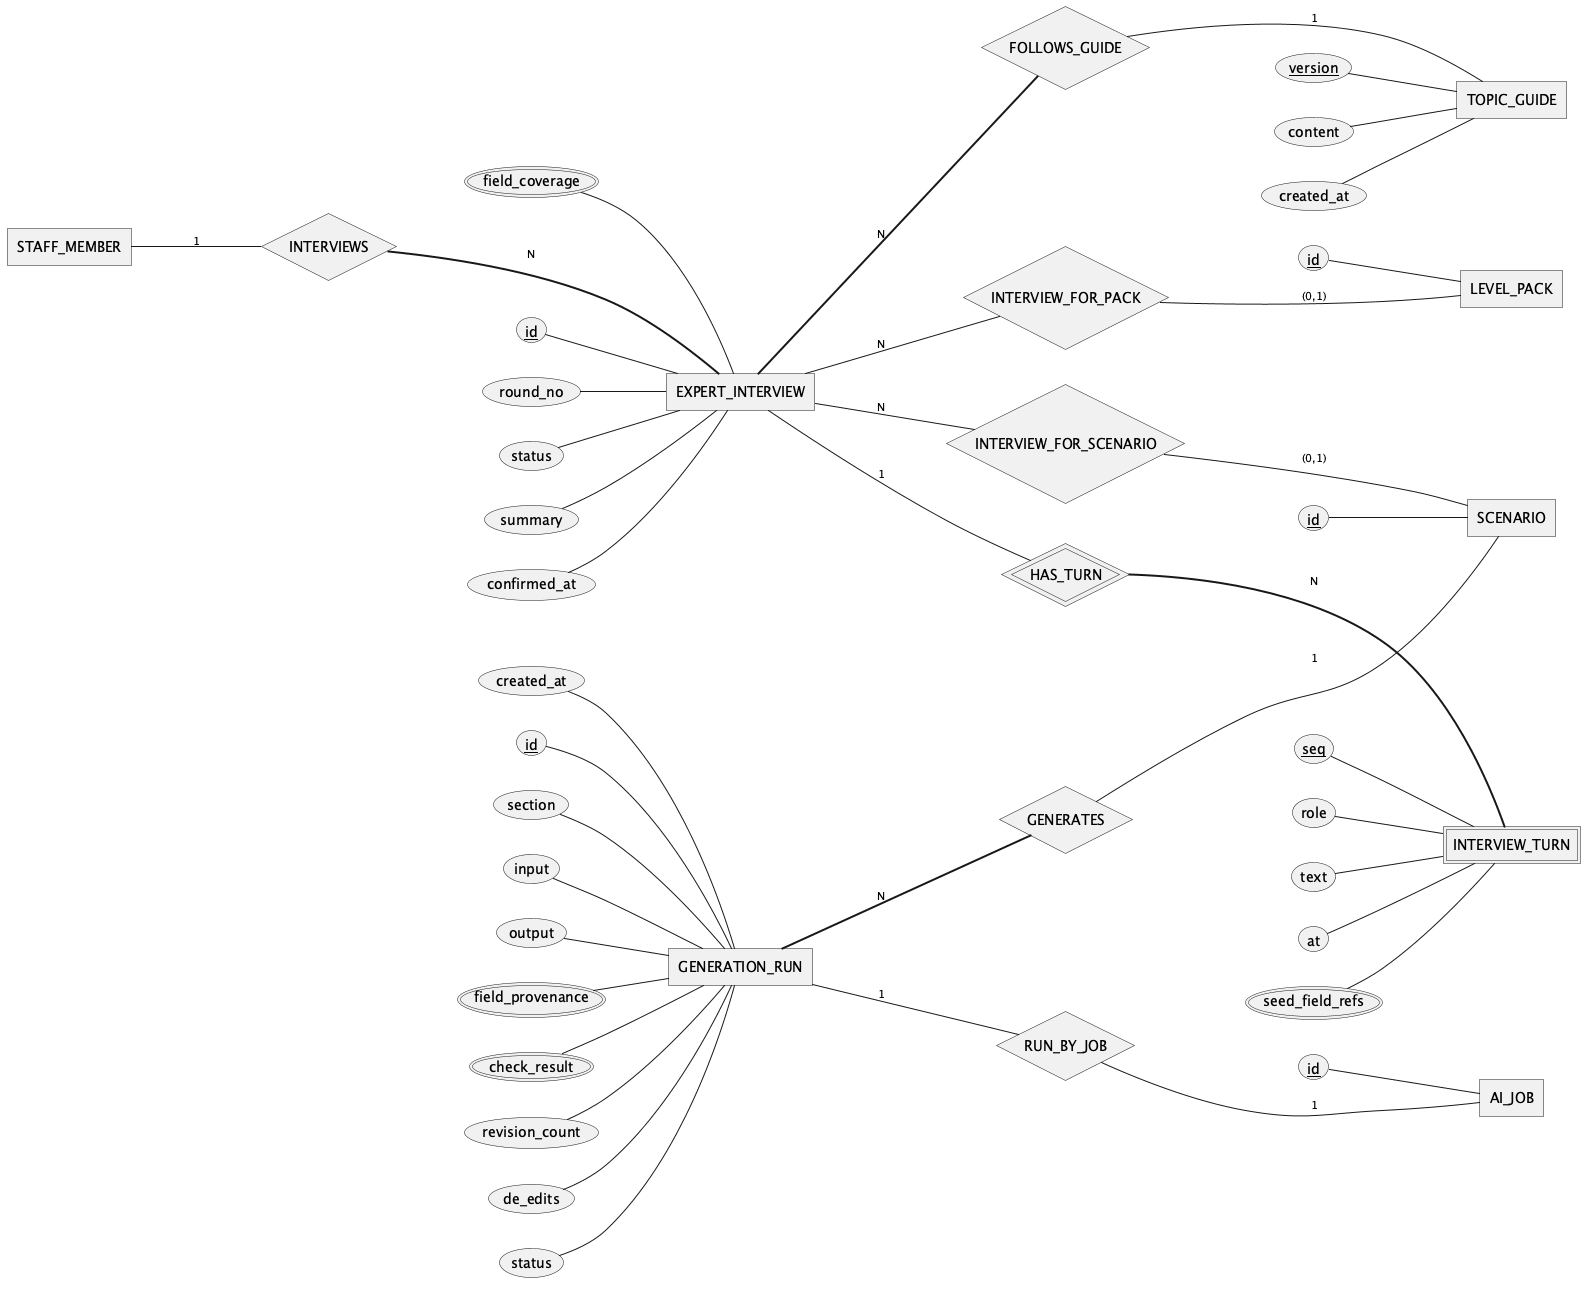
\includegraphics[width=\linewidth,height=0.86\textwidth,keepaspectratio,keepaspectratio]{figures/ERD-04a_InterviewAndDrafting.png}
\caption{Entity--relationship diagram ERD-04a: Interview and AI drafting}
\end{figure}
\end{landscape}

\begin{landscape}
\begin{figure}[H]
\centering
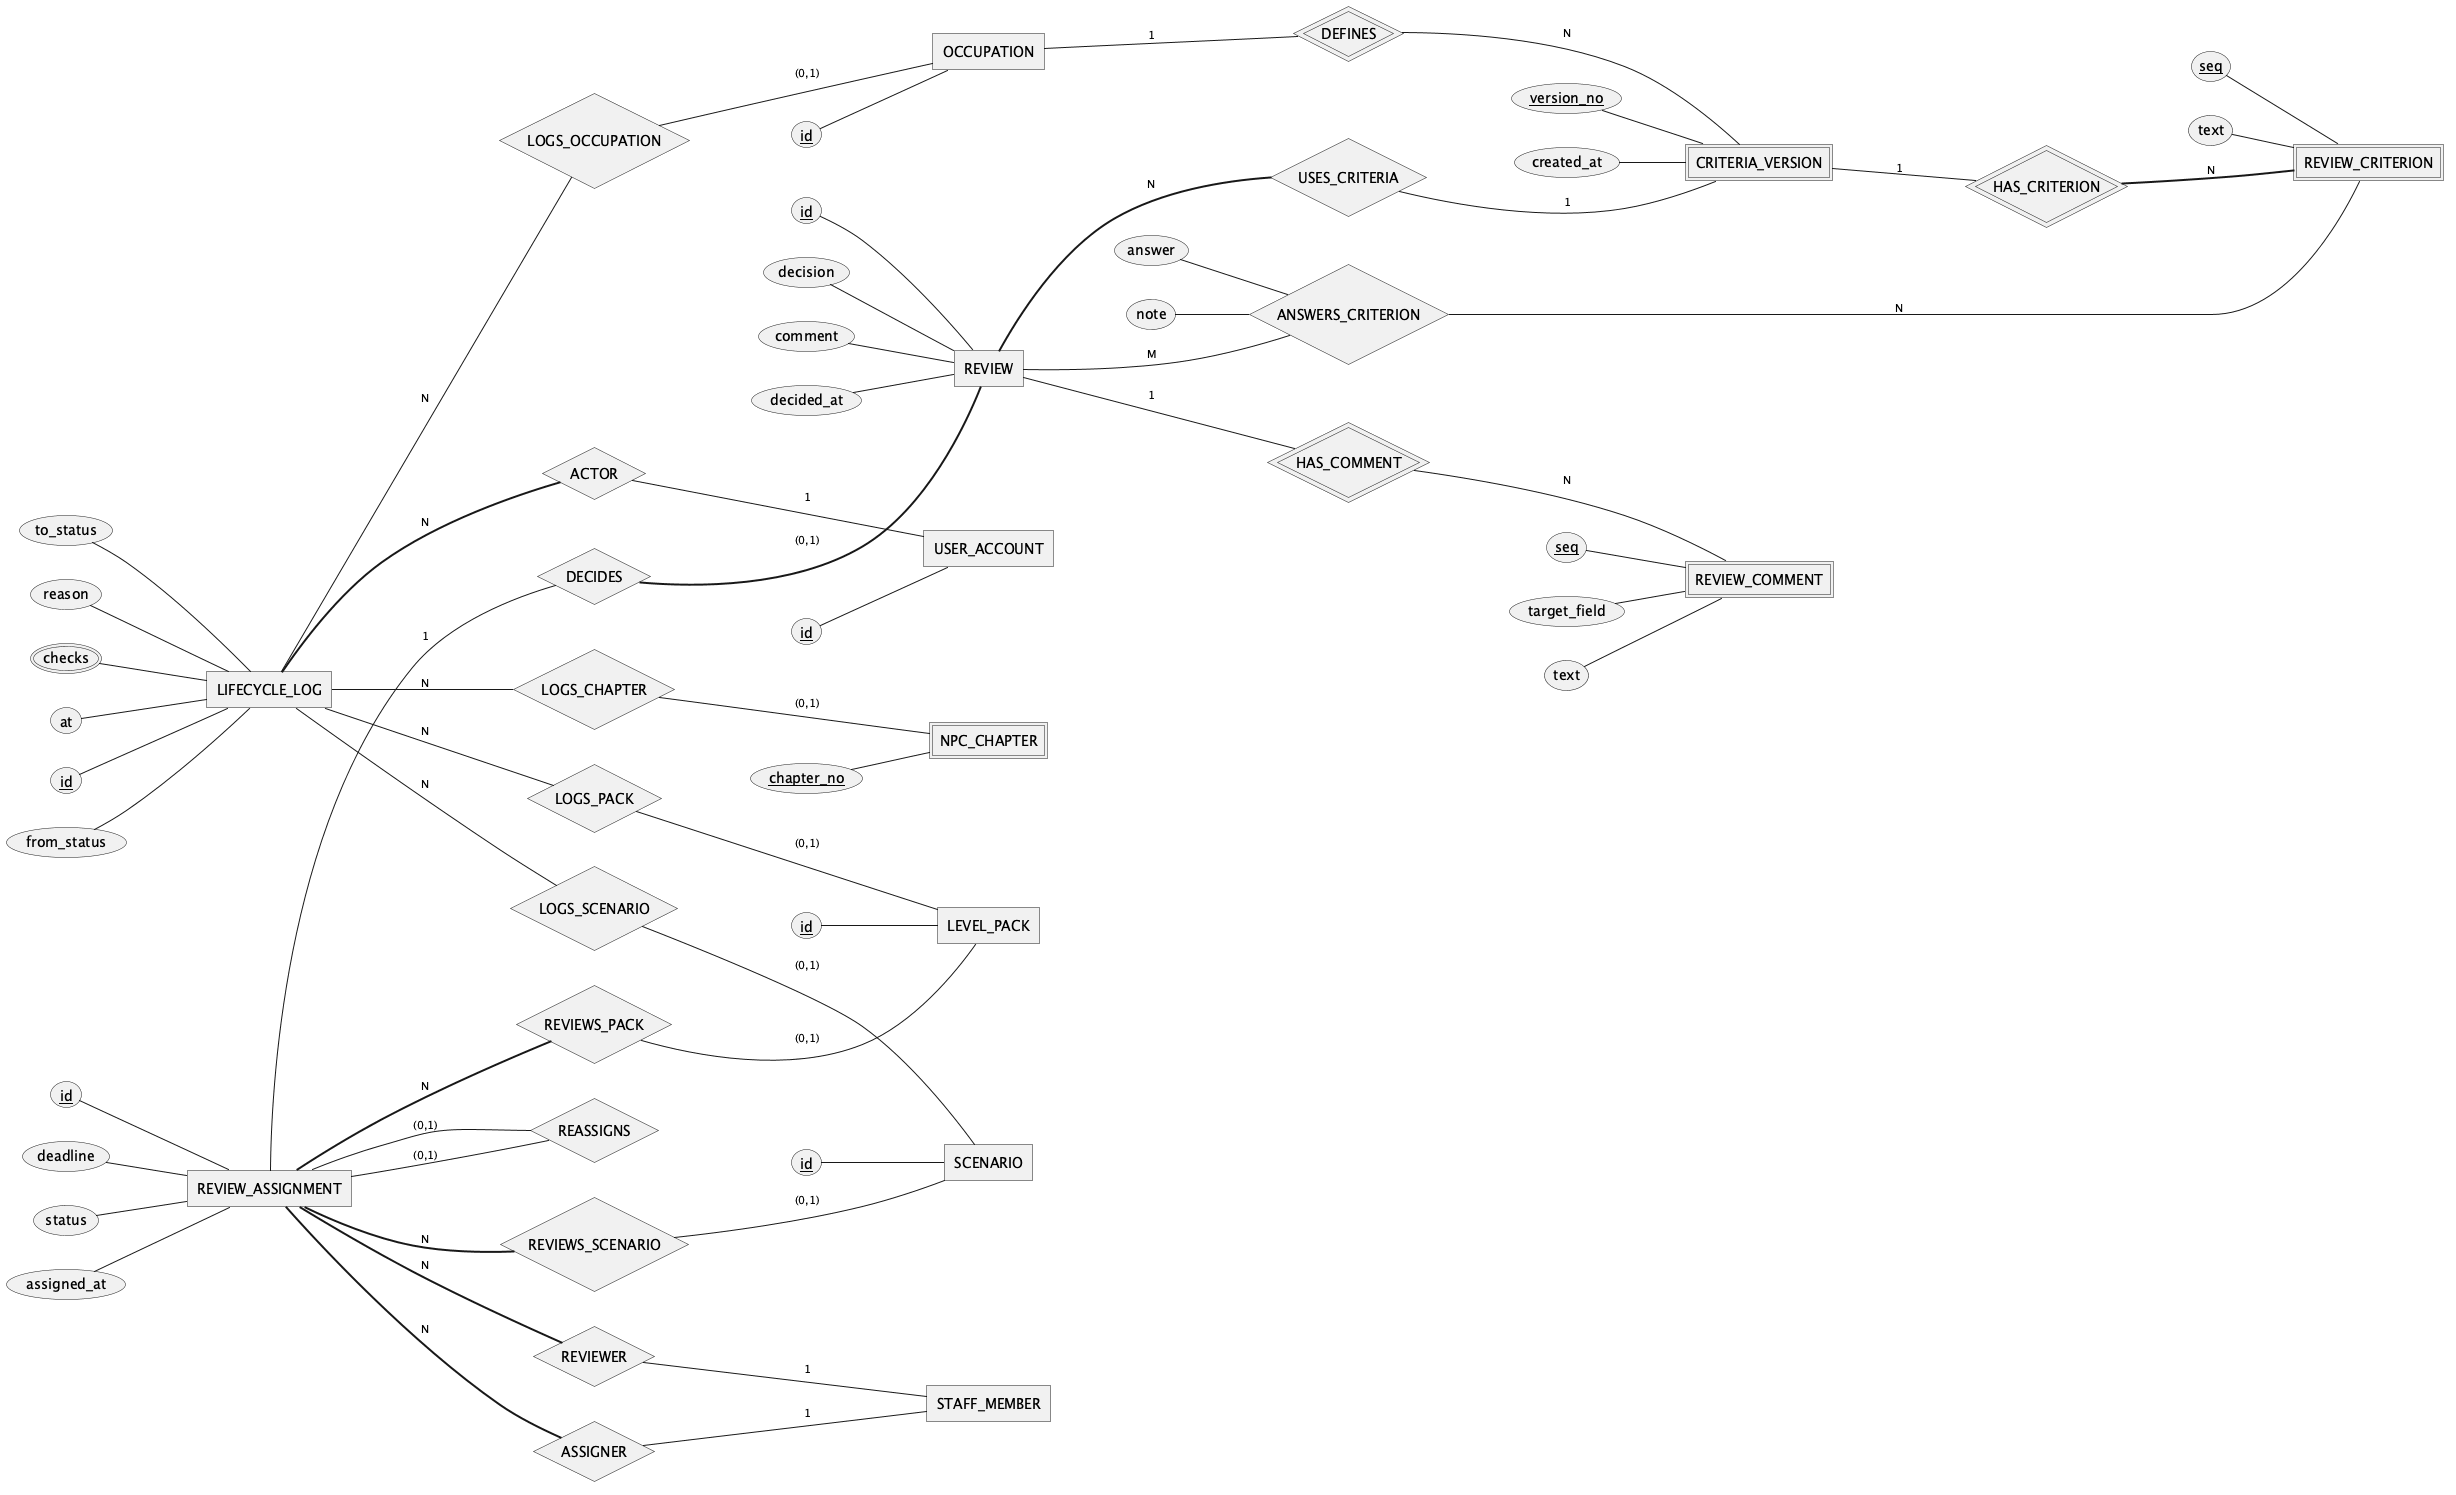
\includegraphics[width=\linewidth,height=0.86\textwidth,keepaspectratio,keepaspectratio]{figures/ERD-04b_ReviewAndLifecycle.png}
\caption{Entity--relationship diagram ERD-04b: Review and lifecycle log}
\end{figure}
\end{landscape}

\begin{landscape}
\begin{figure}[H]
\centering
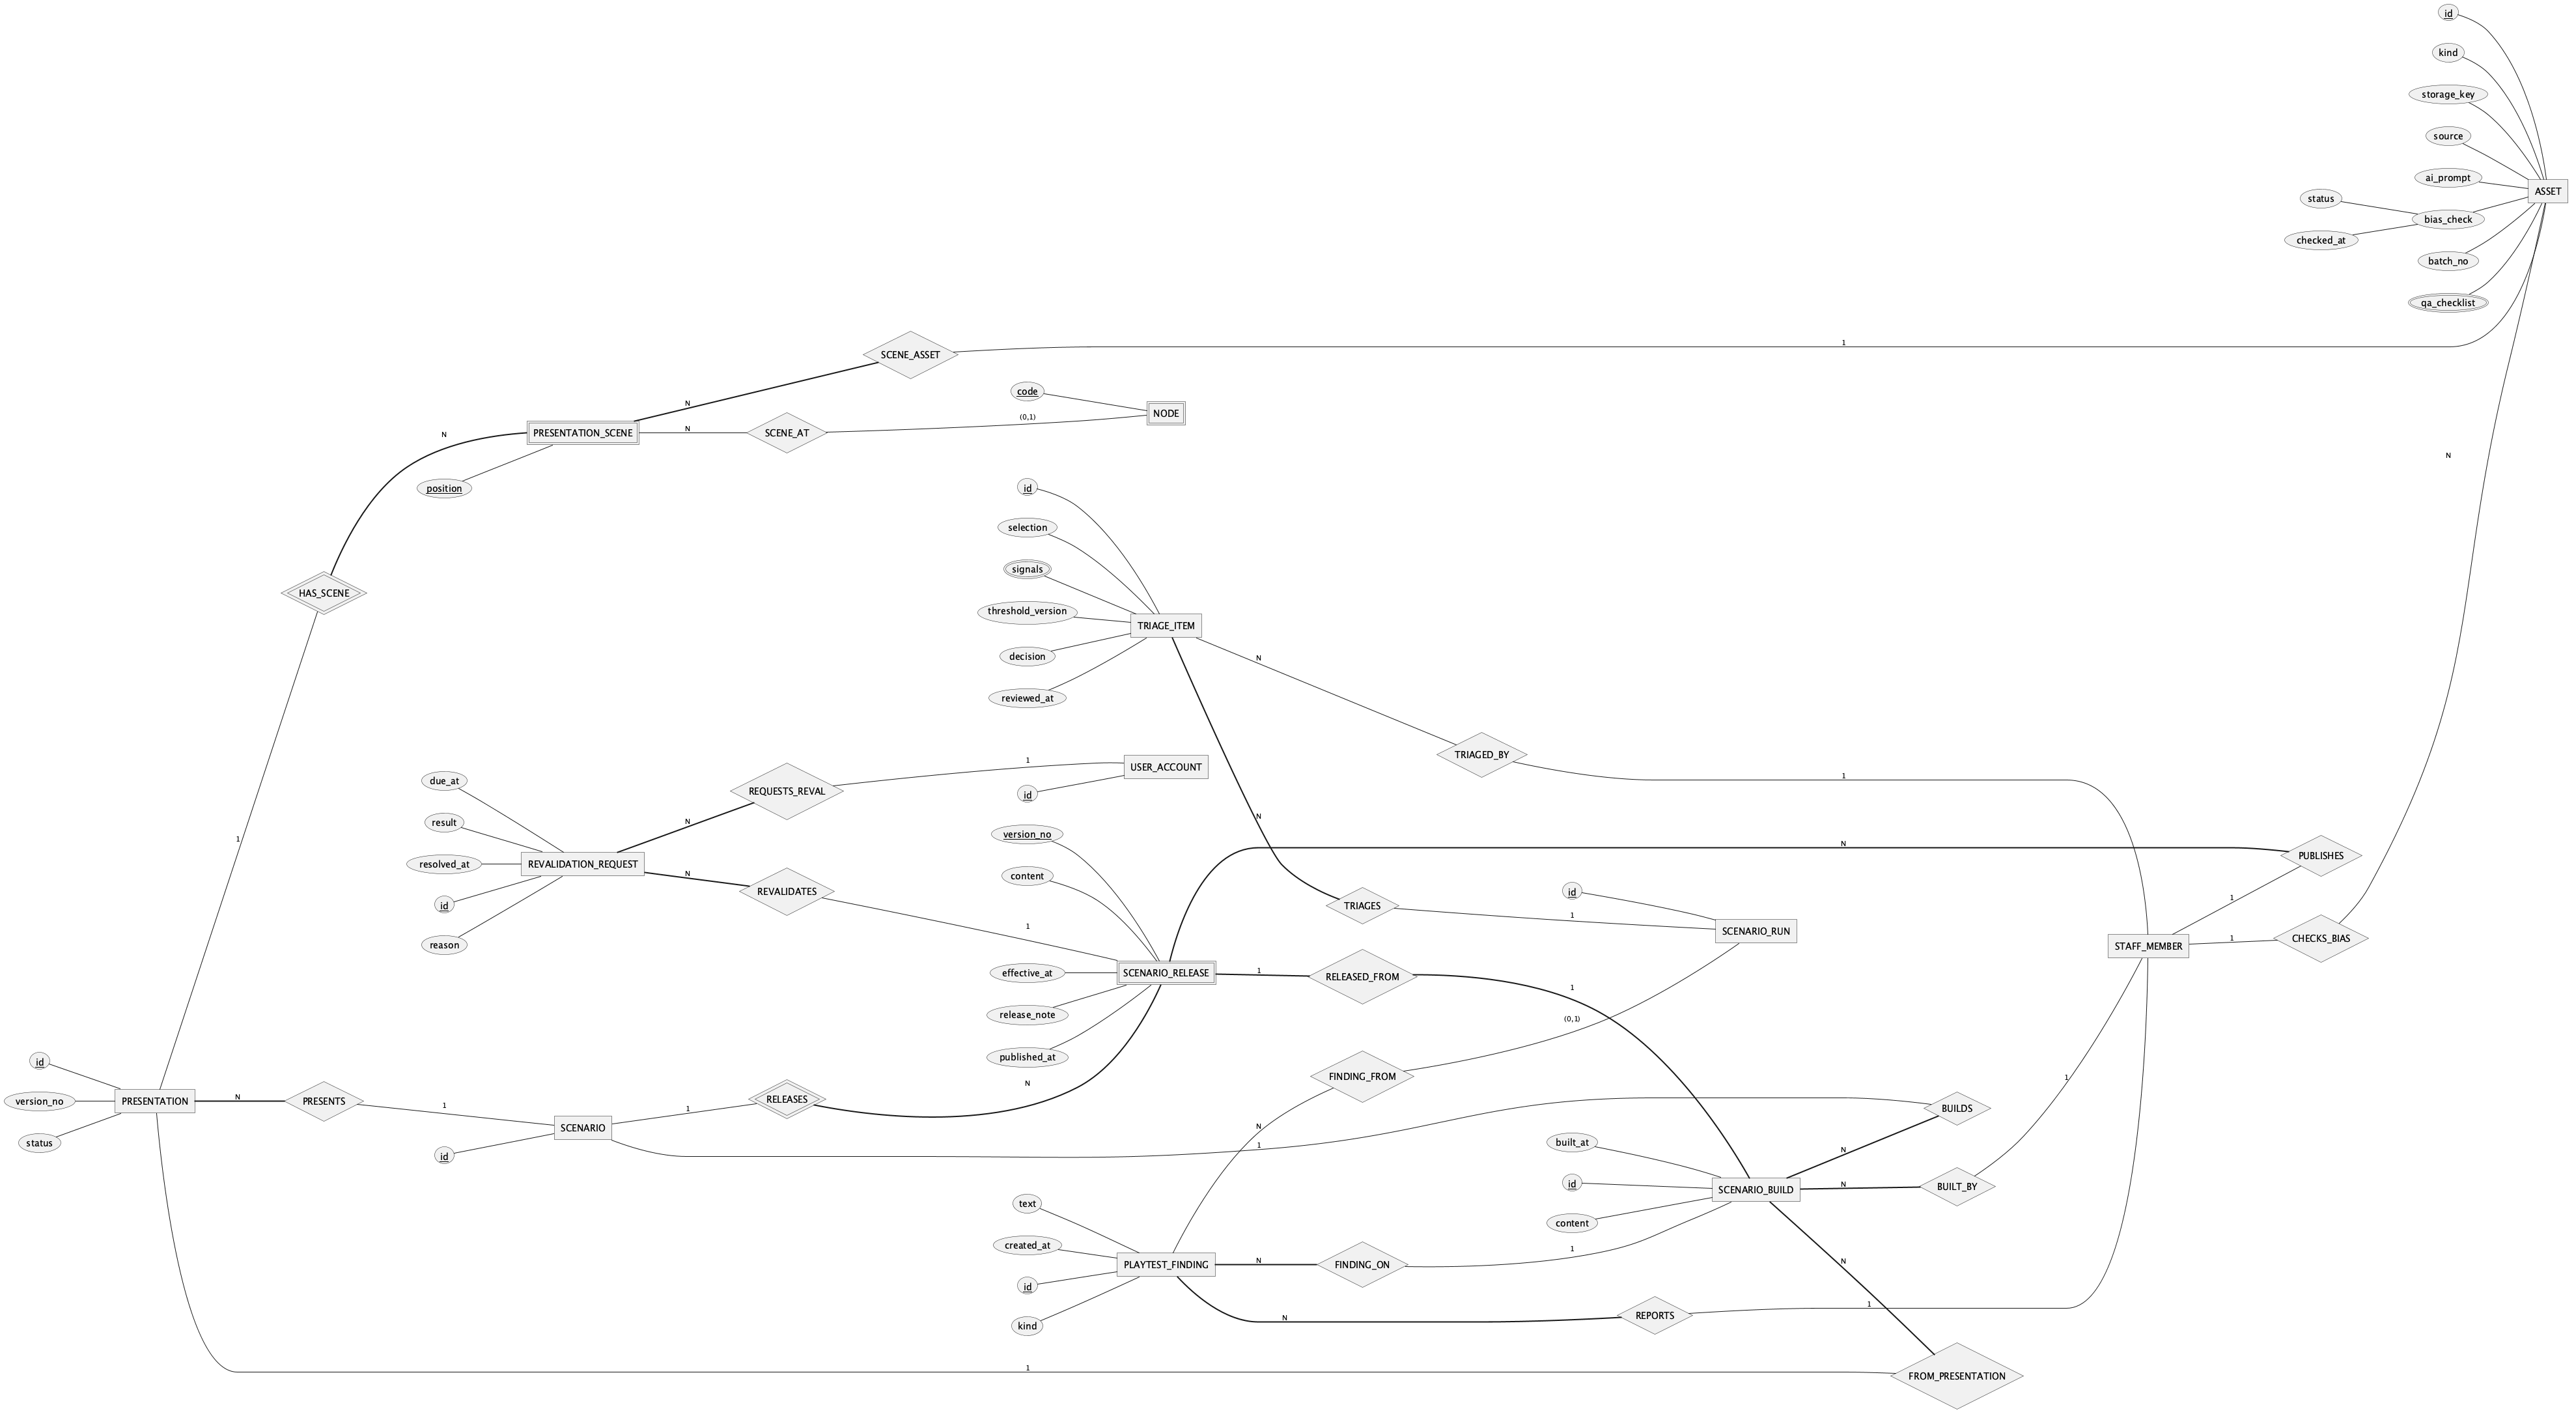
\includegraphics[width=\linewidth,height=0.86\textwidth,keepaspectratio,keepaspectratio]{figures/ERD-04c_PresentationAndRelease.png}
\caption{Entity--relationship diagram ERD-04c: Presentation, play-test and release}
\end{figure}
\end{landscape}

\begin{figure}[H]
\centering
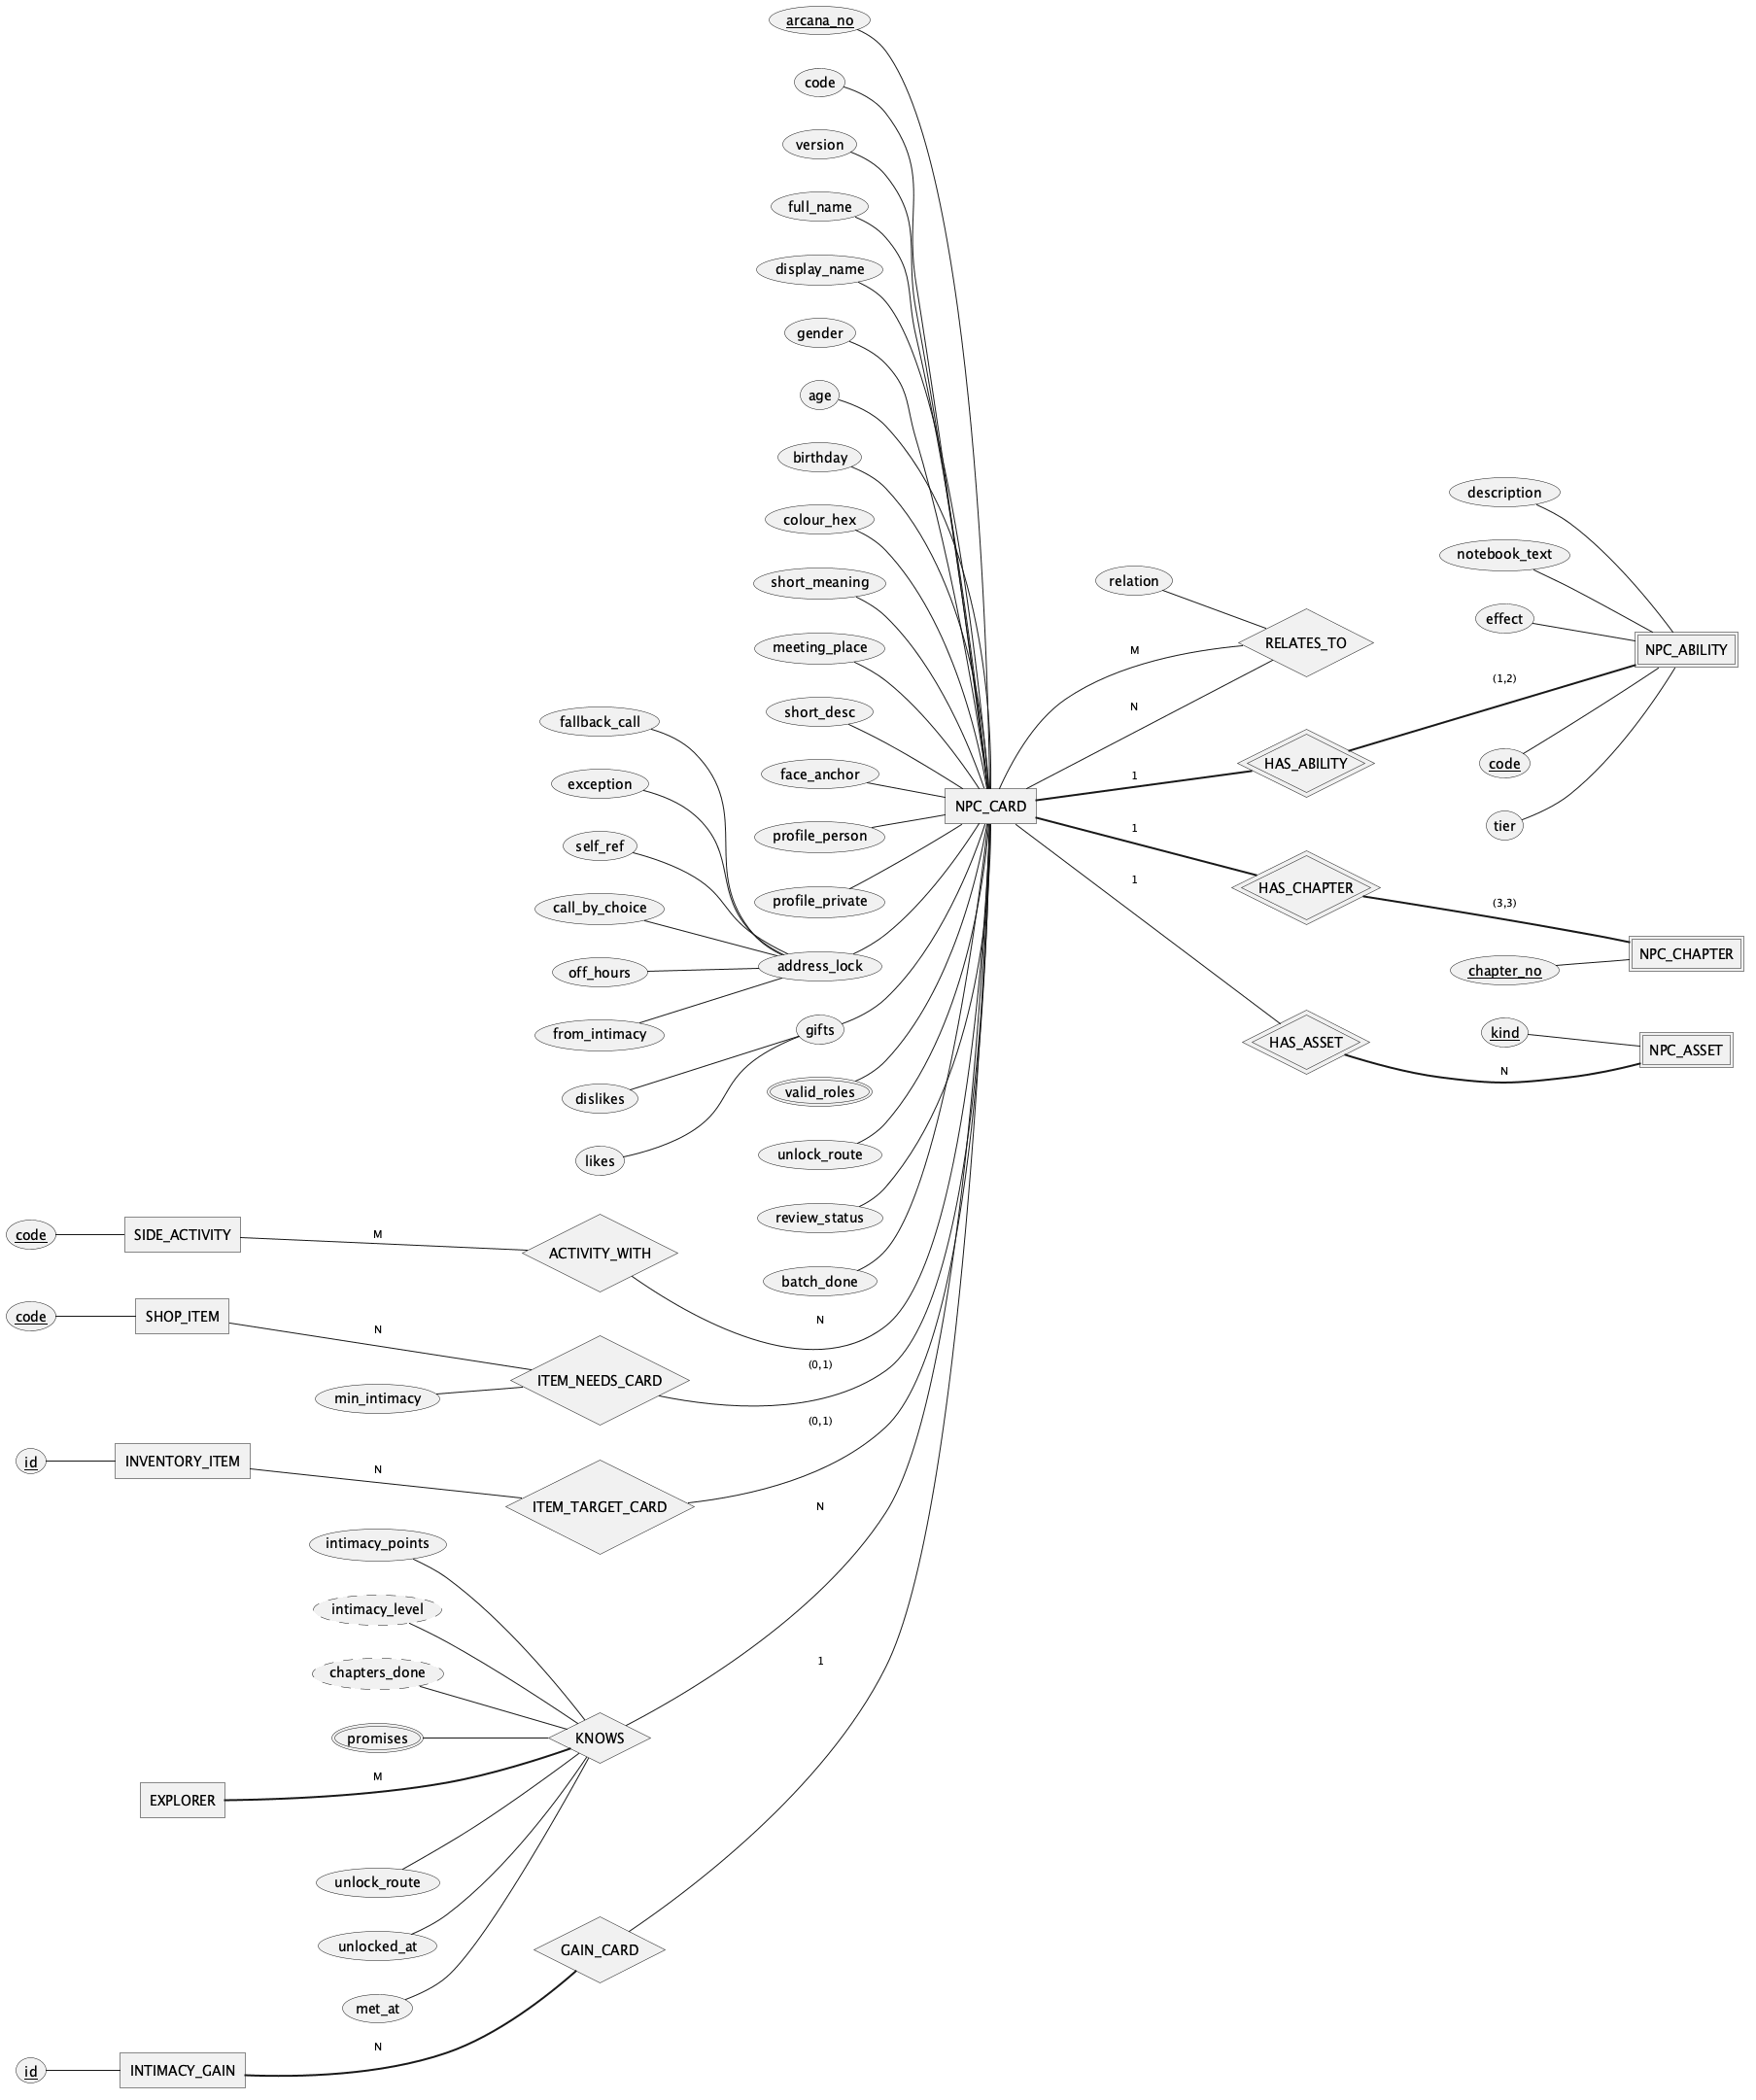
\includegraphics[width=\textwidth,height=0.9\textheight,keepaspectratio]{figures/ERD-05a_NpcCards.png}
\caption{Entity--relationship diagram ERD-05a: Tarot NPC cards}
\end{figure}

\begin{figure}[H]
\centering
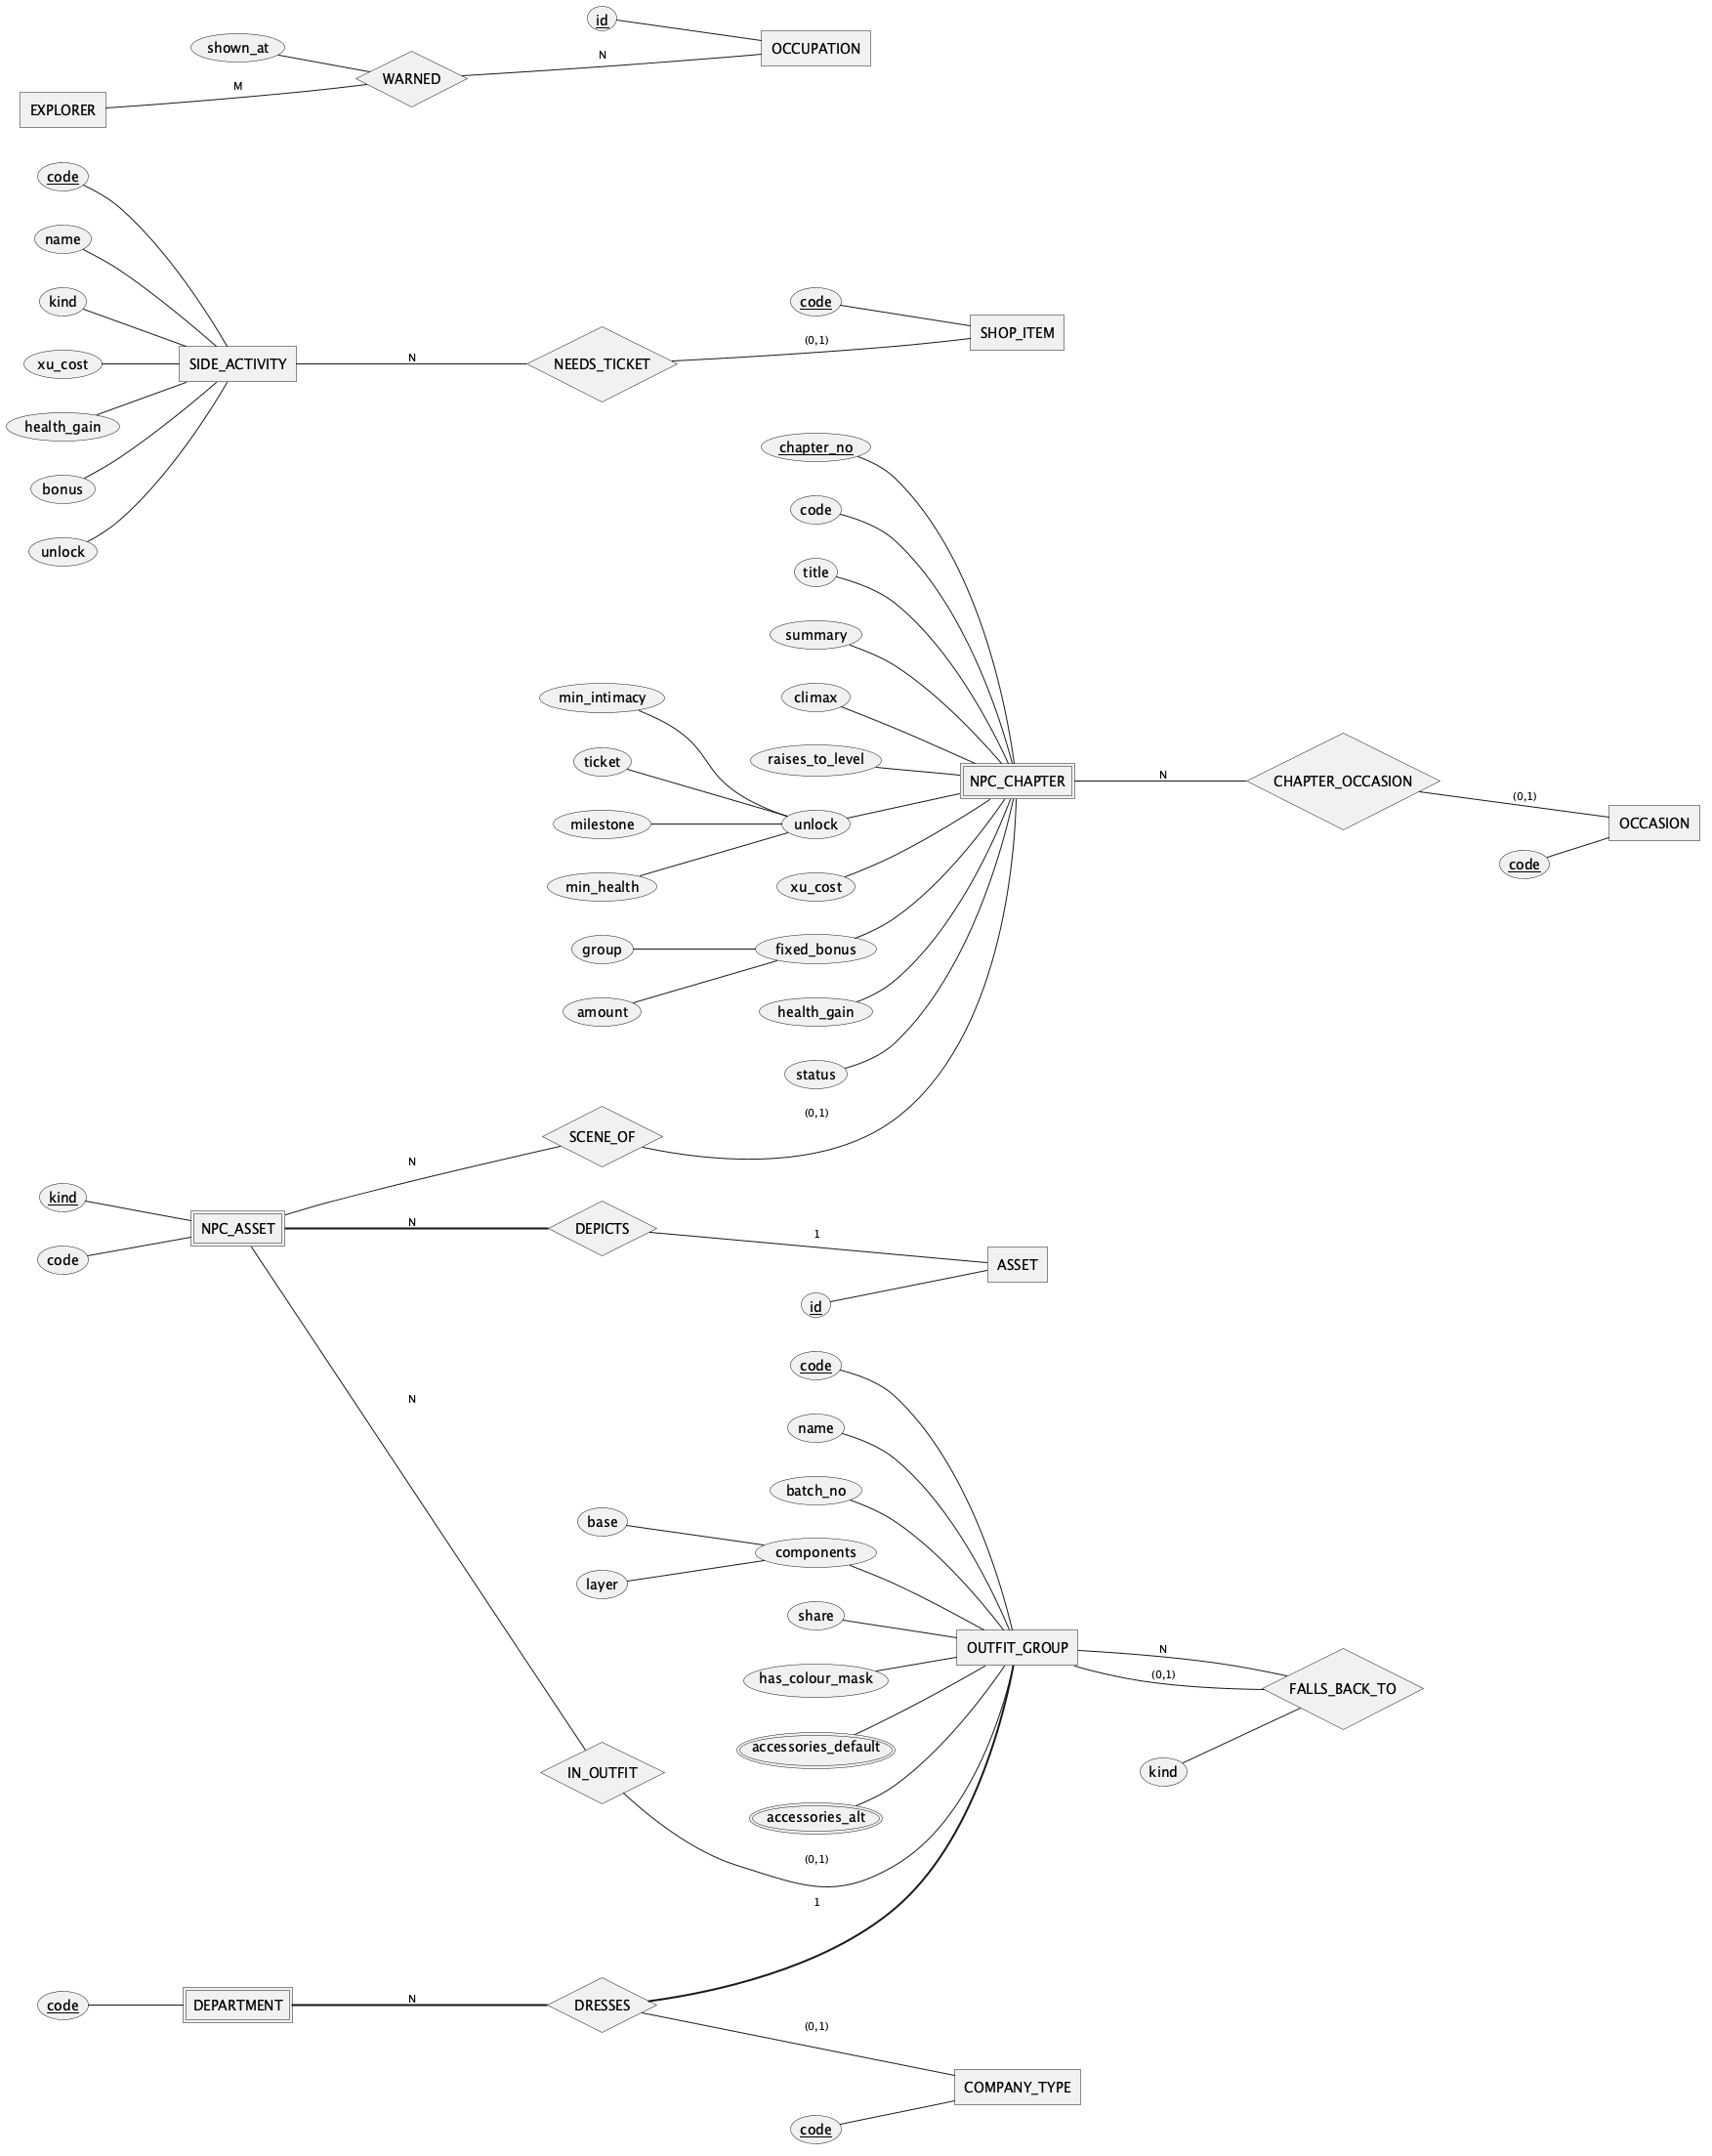
\includegraphics[width=\textwidth,height=0.9\textheight,keepaspectratio]{figures/ERD-05b_NpcChaptersAndSideQuests.png}
\caption{Entity--relationship diagram ERD-05b: NPC chapters, outfits and side quests}
\end{figure}

\begin{landscape}
\begin{figure}[H]
\centering
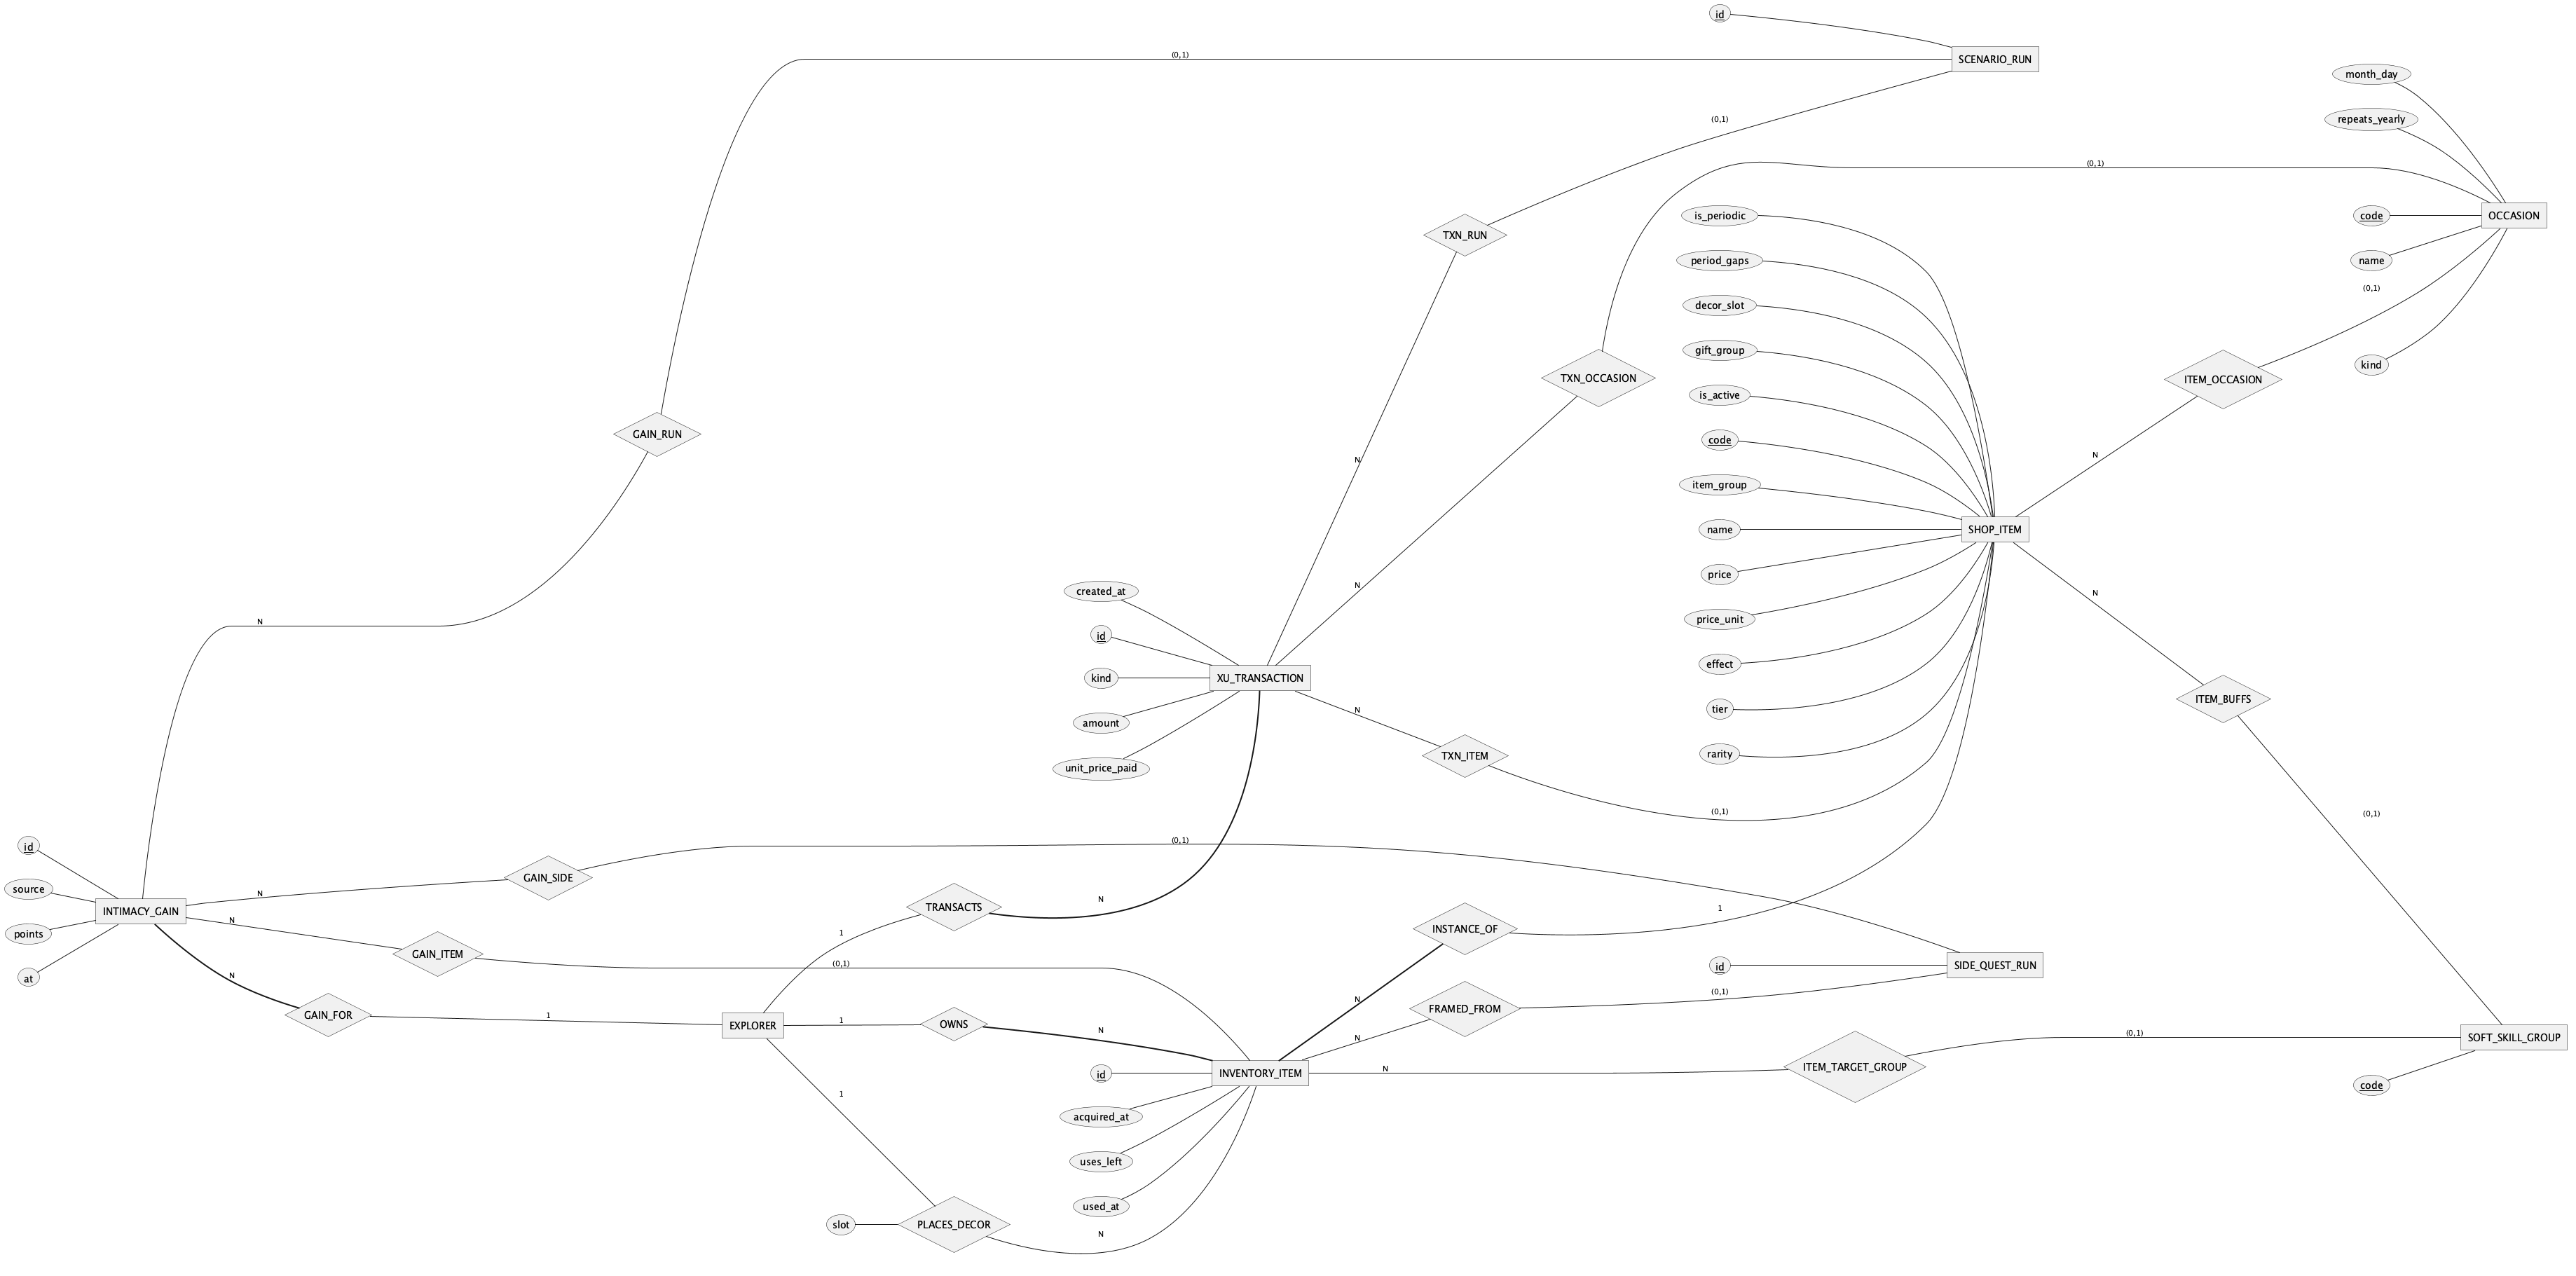
\includegraphics[width=\linewidth,height=0.86\textwidth,keepaspectratio,keepaspectratio]{figures/ERD-05c_Economy.png}
\caption{Entity--relationship diagram ERD-05c: Economy and inventory}
\end{figure}
\end{landscape}

\begin{landscape}
\begin{figure}[H]
\centering
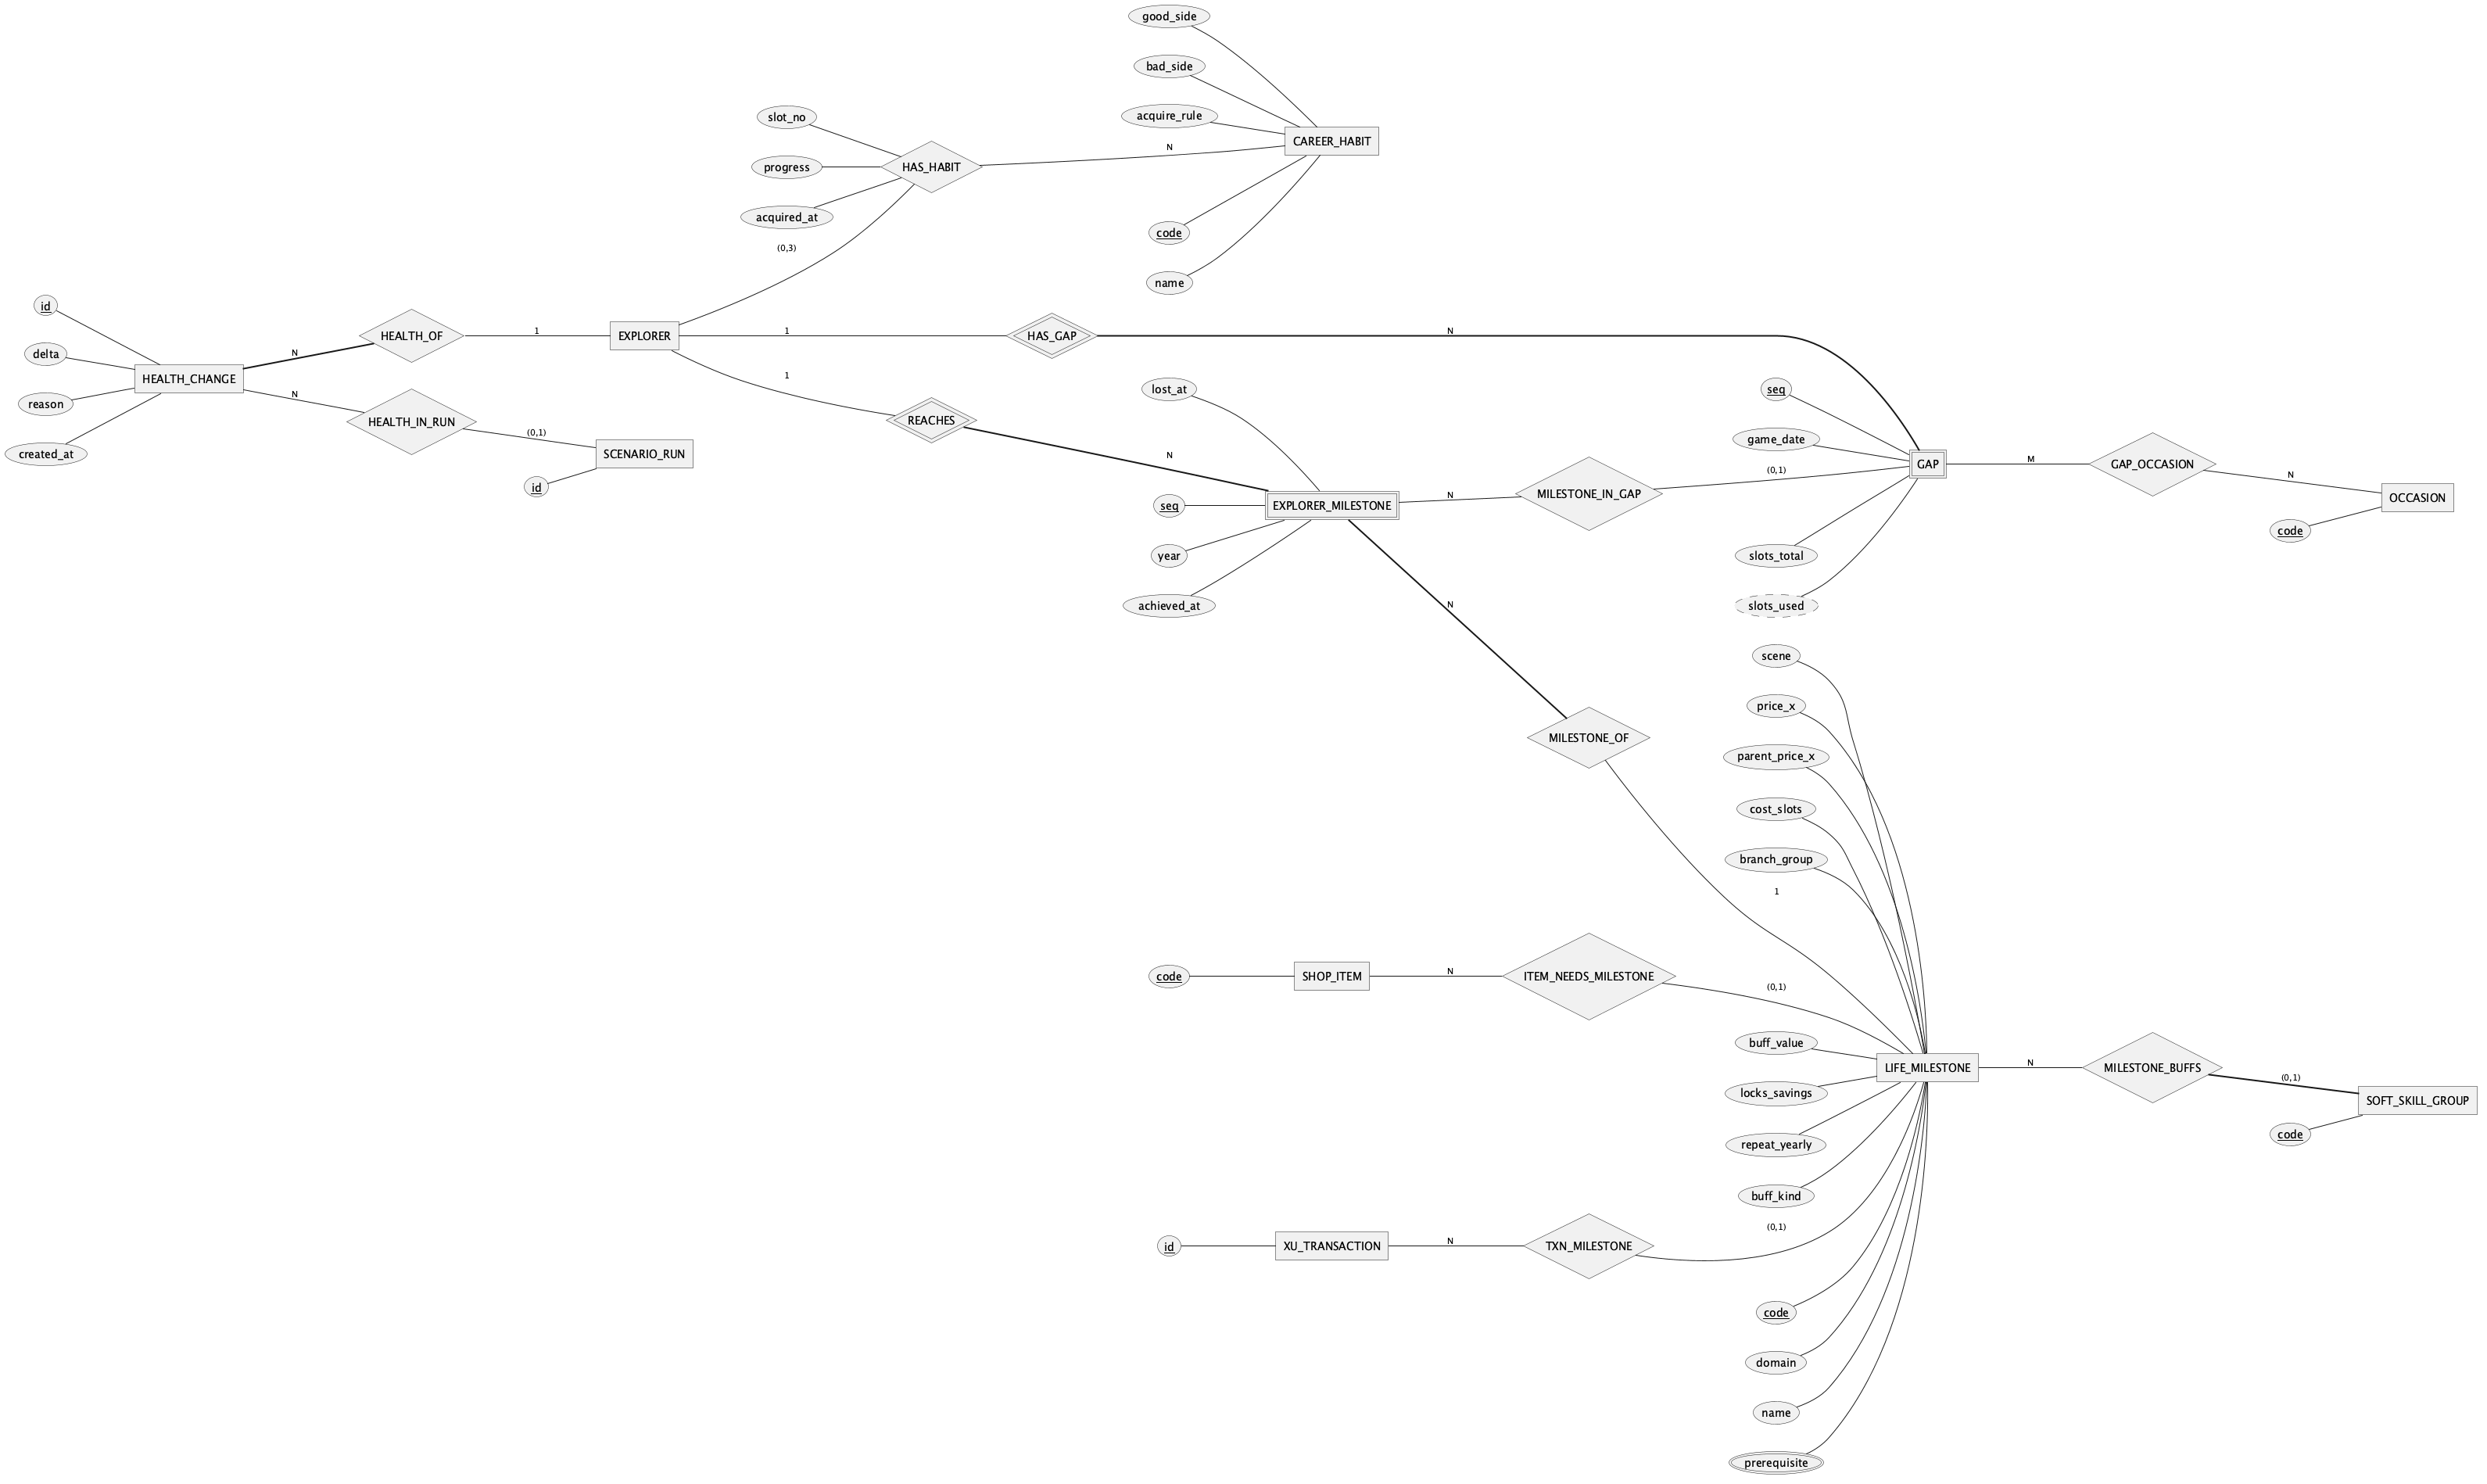
\includegraphics[width=\linewidth,height=0.86\textwidth,keepaspectratio,keepaspectratio]{figures/ERD-05d_HealthAndLife.png}
\caption{Entity--relationship diagram ERD-05d: Health, habits and life milestones}
\end{figure}
\end{landscape}

\begin{landscape}
\begin{figure}[H]
\centering
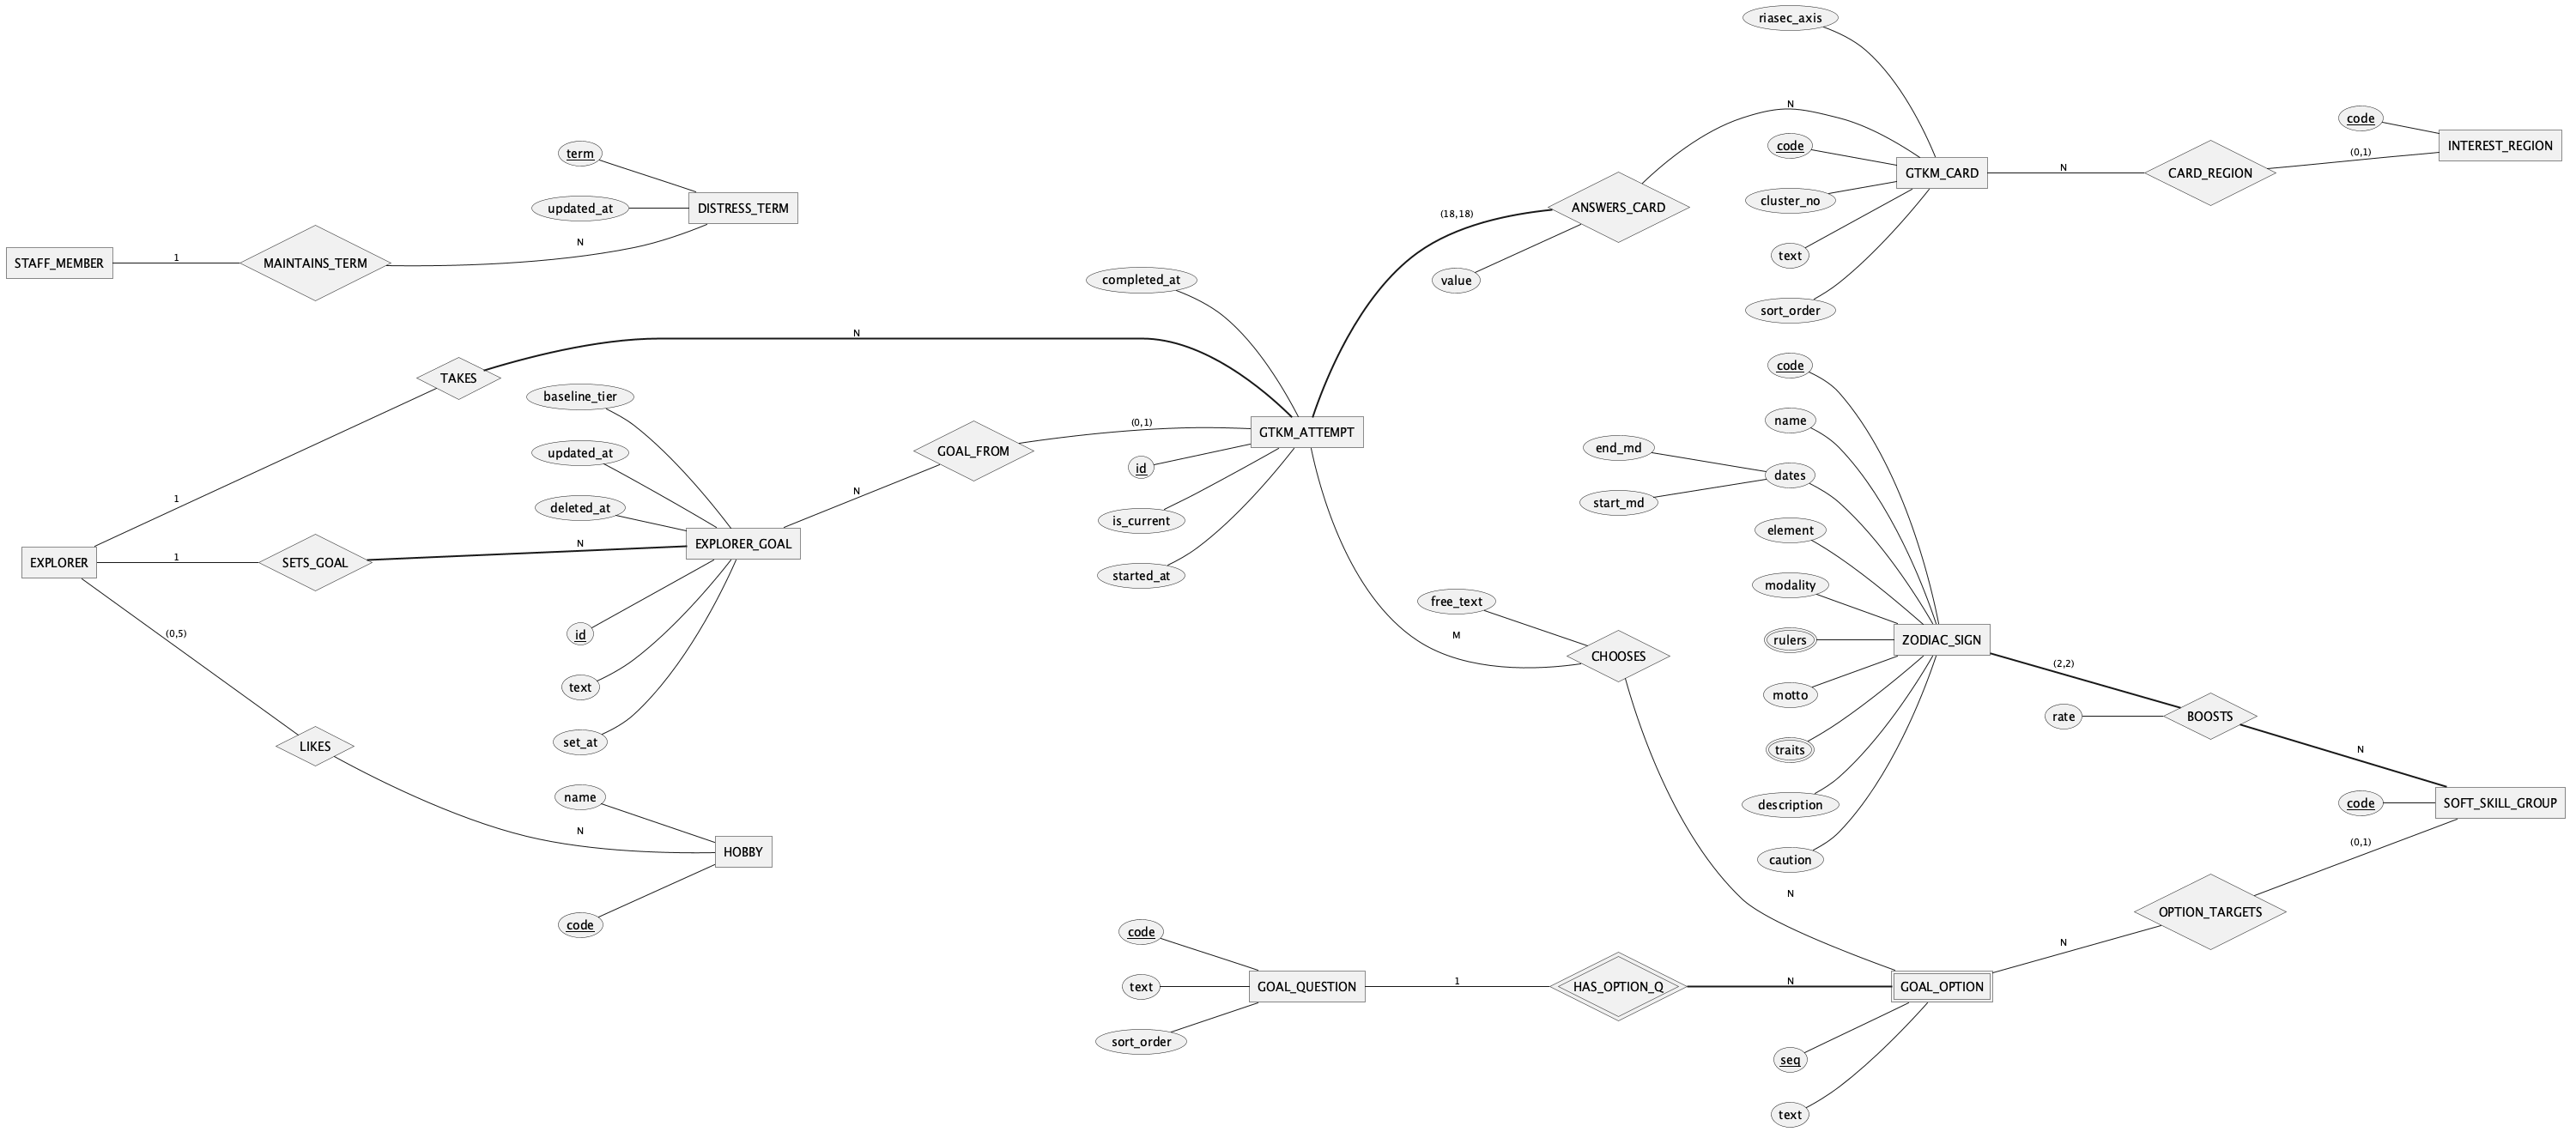
\includegraphics[width=\linewidth,height=0.86\textwidth,keepaspectratio,keepaspectratio]{figures/ERD-06a_ExplorerProfile.png}
\caption{Entity--relationship diagram ERD-06a: Explorer profile}
\end{figure}
\end{landscape}

\begin{landscape}
\begin{figure}[H]
\centering
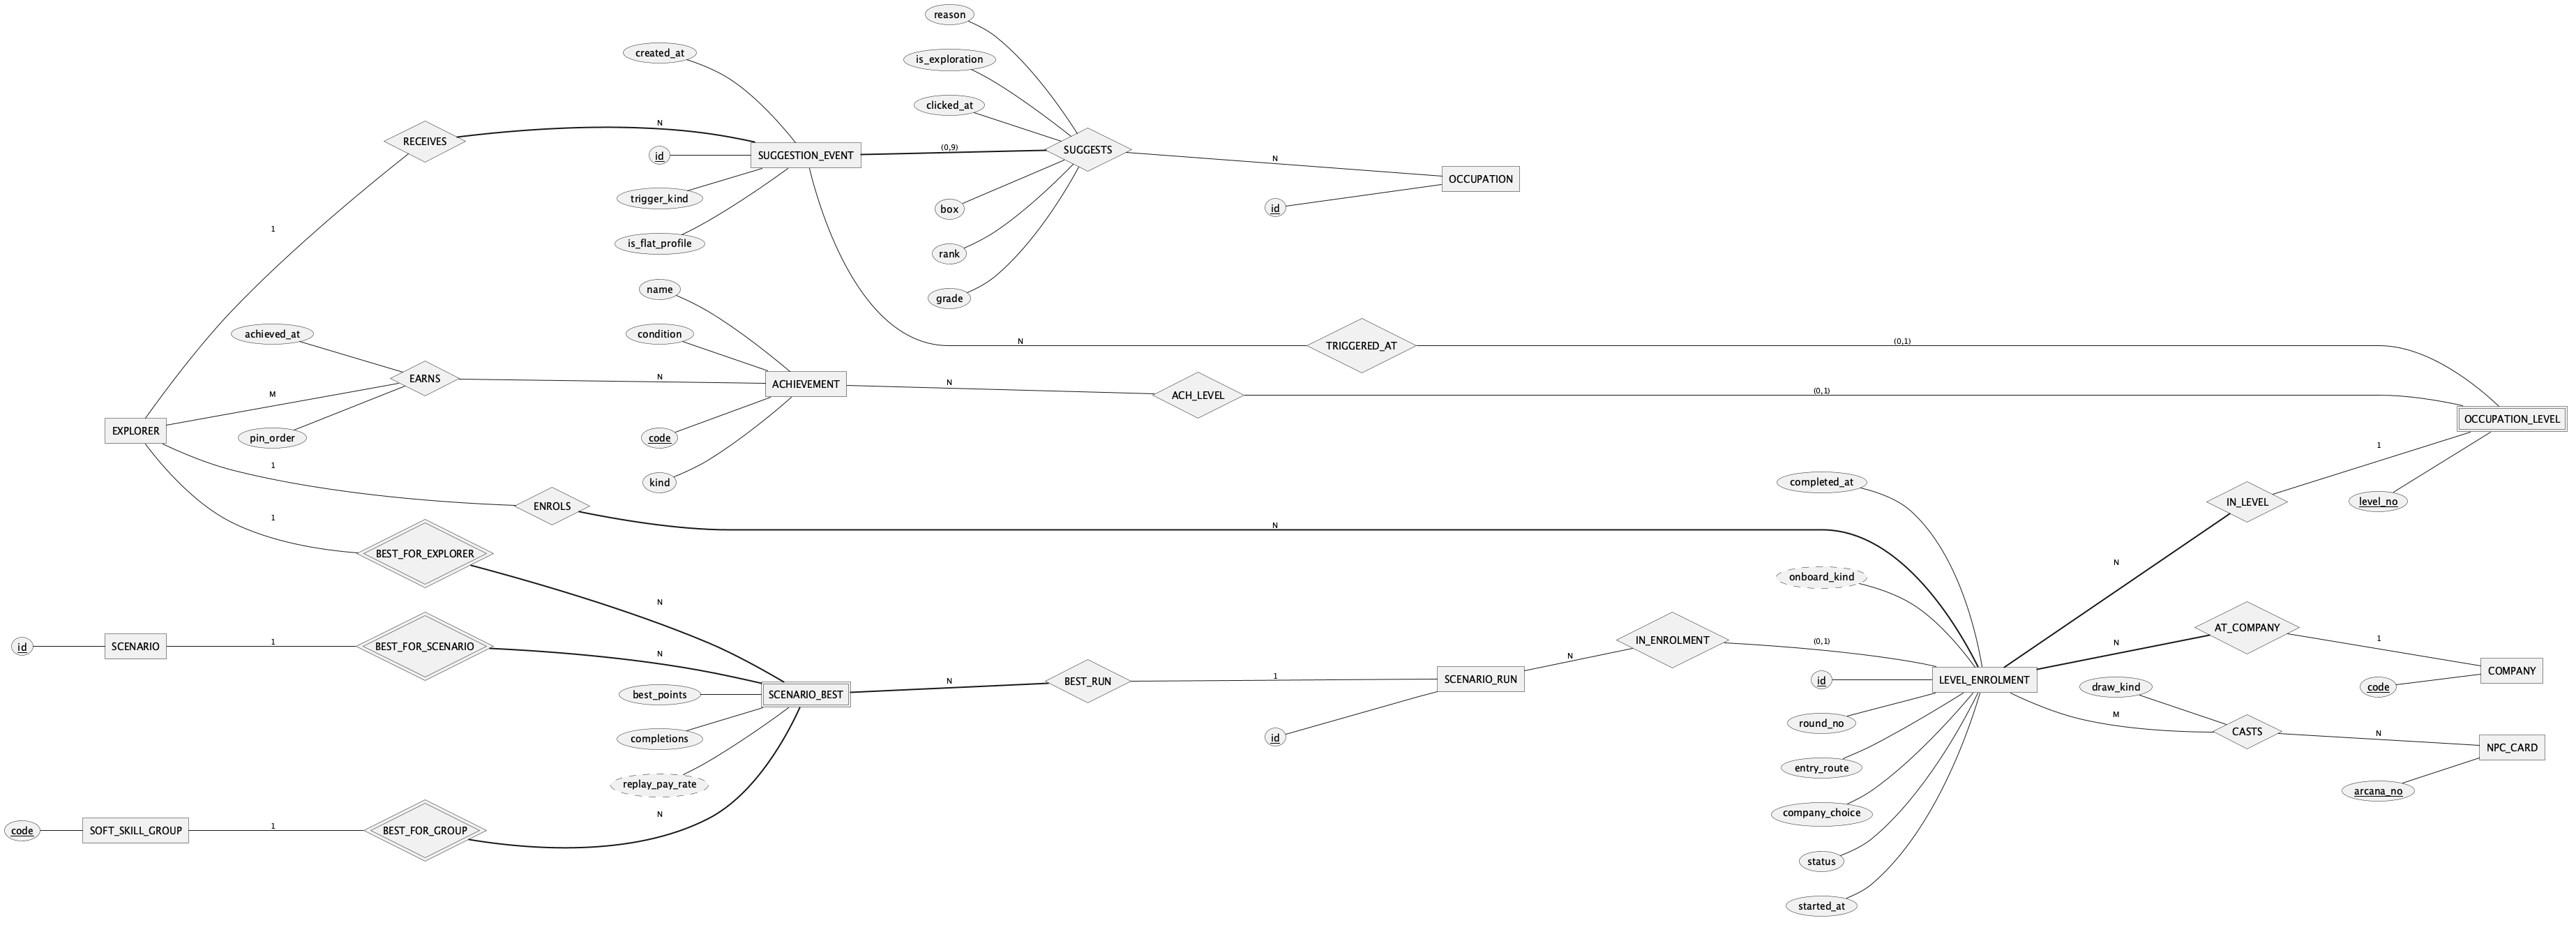
\includegraphics[width=\linewidth,height=0.86\textwidth,keepaspectratio,keepaspectratio]{figures/ERD-06b_Progression.png}
\caption{Entity--relationship diagram ERD-06b: Progression}
\end{figure}
\end{landscape}

\begin{landscape}
\begin{figure}[H]
\centering
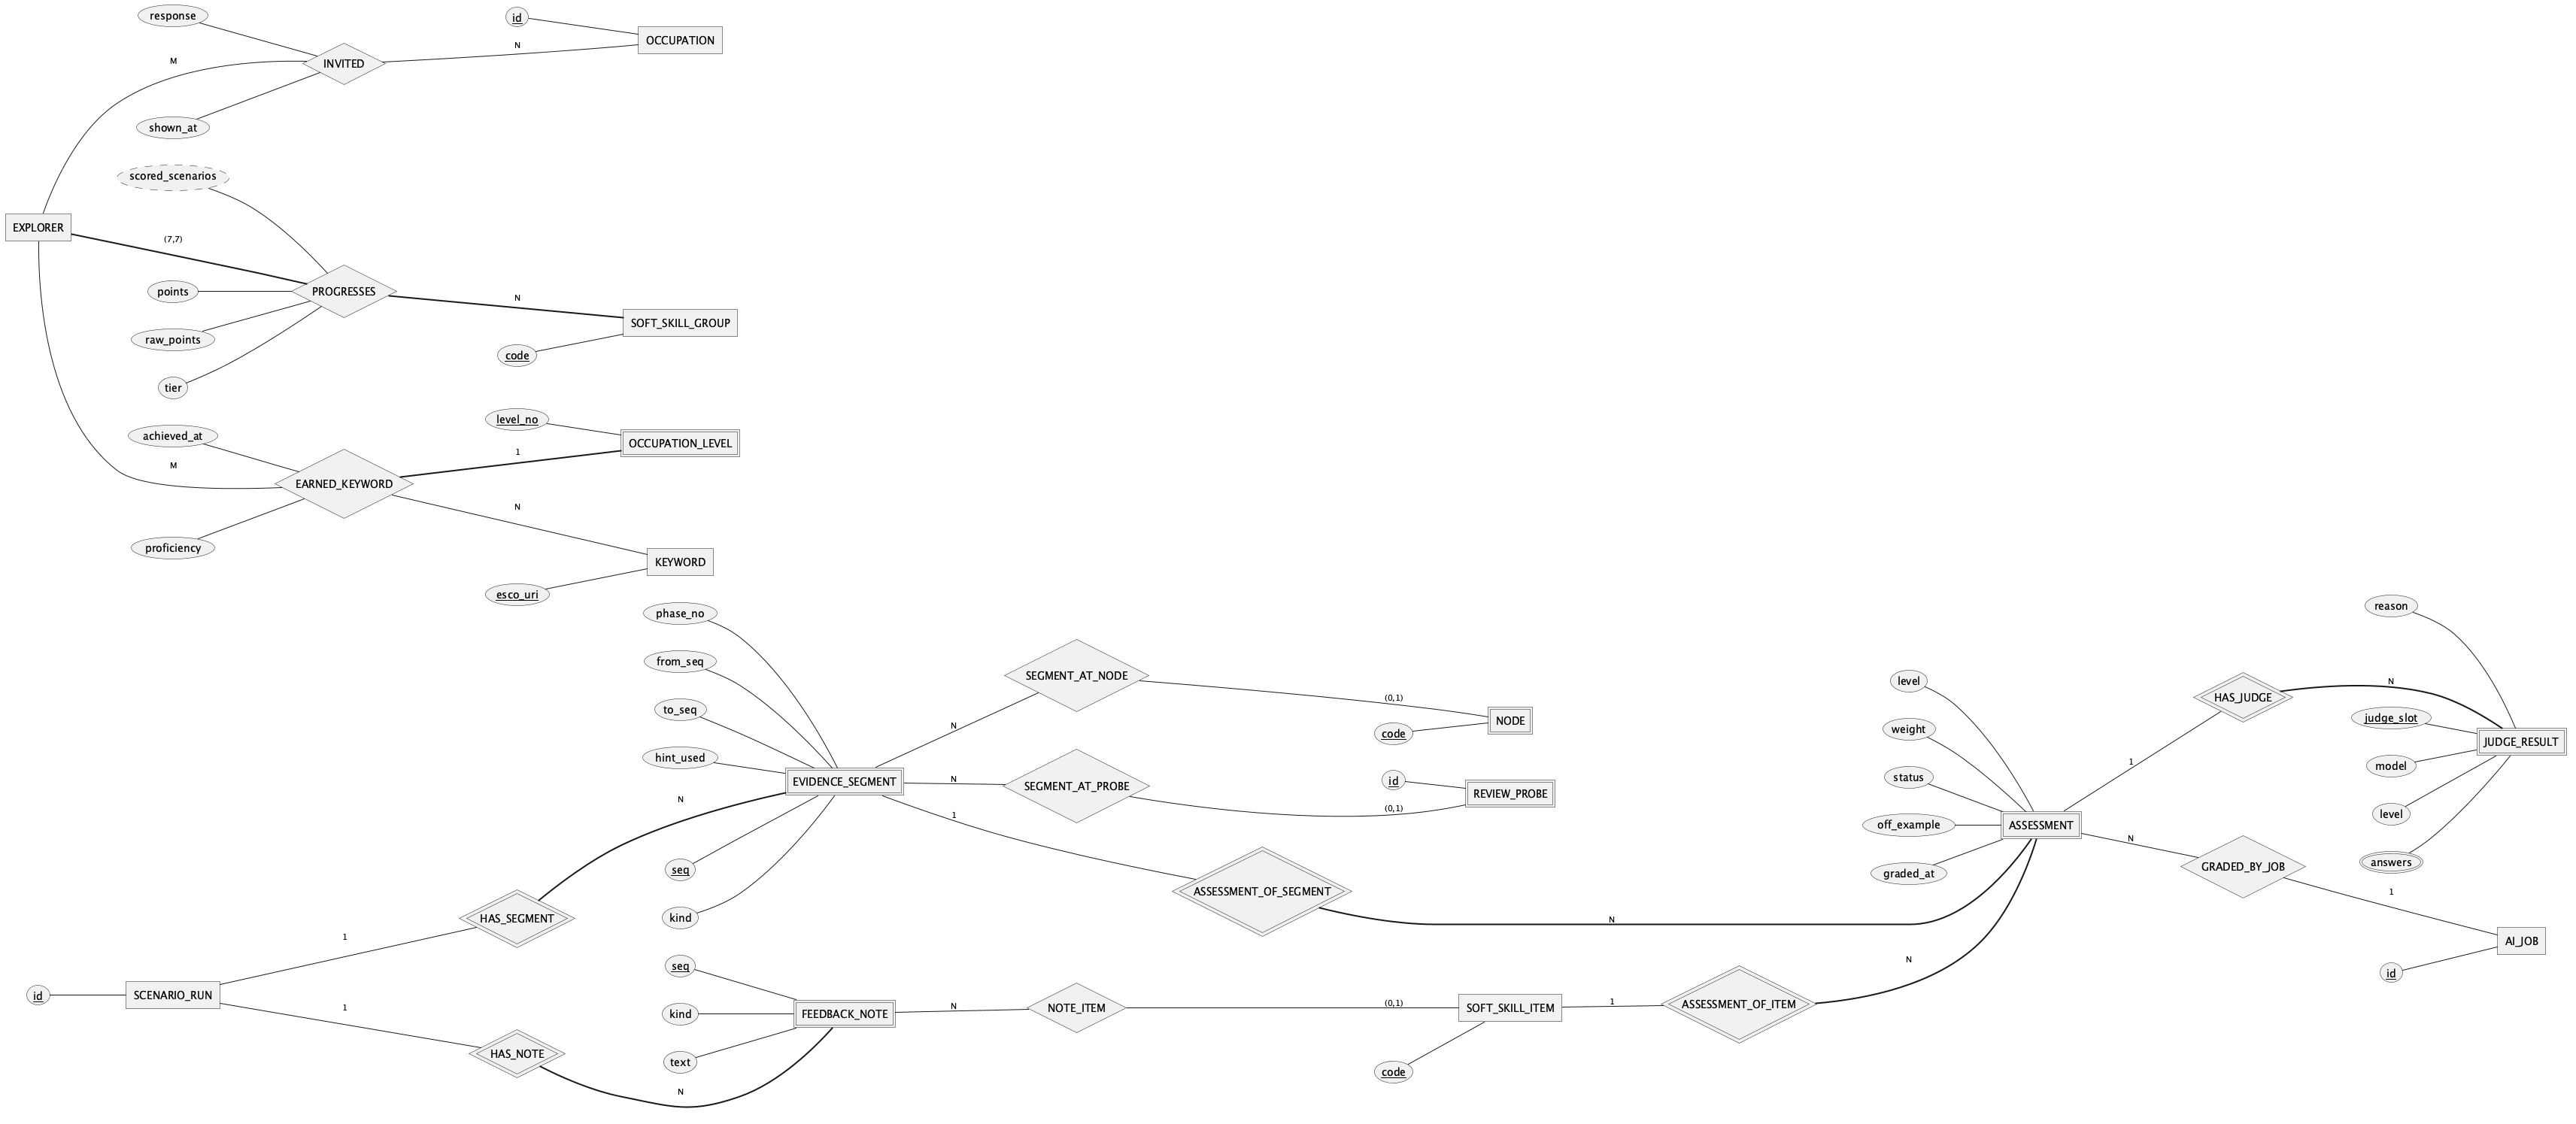
\includegraphics[width=\linewidth,height=0.86\textwidth,keepaspectratio,keepaspectratio]{figures/ERD-06d_Grading.png}
\caption{Entity--relationship diagram ERD-06d: Evidence and grading}
\end{figure}
\end{landscape}

Repository packages.

\begin{figure}[H]
\centering
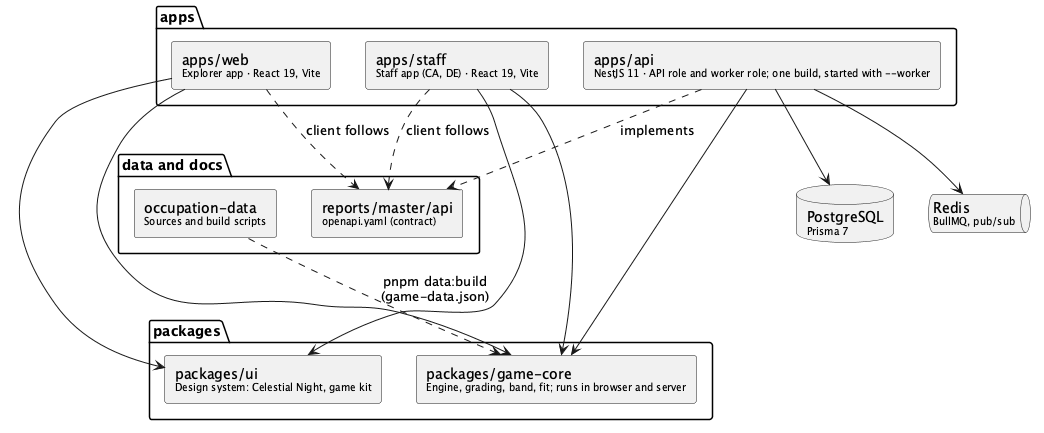
\includegraphics[width=0.9\textwidth,height=0.85\textheight,keepaspectratio]{figures/PK-01_RepositoryPackages.png}
\caption{Repository packages and their dependencies (PK-01)}
\end{figure}
